\documentclass[]{article}
\usepackage{xcolor}
\usepackage{listings}
\usepackage{graphicx}
\graphicspath{{./}}
\definecolor{codegreen}{rgb}{0,0.6,0}
\definecolor{codegray}{rgb}{0.5,0.5,0.5}
\definecolor{codepurple}{rgb}{0.58,0,0.82}
\definecolor{backcolour}{rgb}{0.95,0.95,0.92}
\lstdefinestyle{mystyle}{
    backgroundcolor=\color{backcolour},   
    commentstyle=\color{codegreen},
    keywordstyle=\color{magenta},
    numberstyle=\tiny\color{codegray},
    stringstyle=\color{codepurple},
    basicstyle=\ttfamily\footnotesize,
    breakatwhitespace=false,         
    breaklines=true,                 
    captionpos=t,                    
    keepspaces=true,                 
    numbers=left,                    
    numbersep=5pt,                  
    showspaces=false,                
    showstringspaces=false,
    showtabs=false,                  
    tabsize=2
}
\lstset{style=mystyle}

\title{Laporan Praktikum\\Mata Kuliah Sistem Manajemen Basis Data\\SQL Practice}
\author{Dwi Cahya Ramadani}
\date{25 April 2022}

\begin{document}

\maketitle

\section{Soal Easy}
    \begin{itemize}
        \item Show first name, last name, and gender of patients who's gender is 'M'
        \\Query : 
        \lstinputlisting[label={listing1},caption={Easy - 1}, language={sql}]{"../Easy-1.sql"}
        Penjelasan :
        \begin{itemize}
            \item Baris 1 : Mengambil data first\_name, last\_name, dan gender dari tabel patients
            \item Baris 2 : Dengan kondisi dimana gendernya adalah "M"
        \end{itemize}
        Screenshot :
        \begin{figure}[h]
            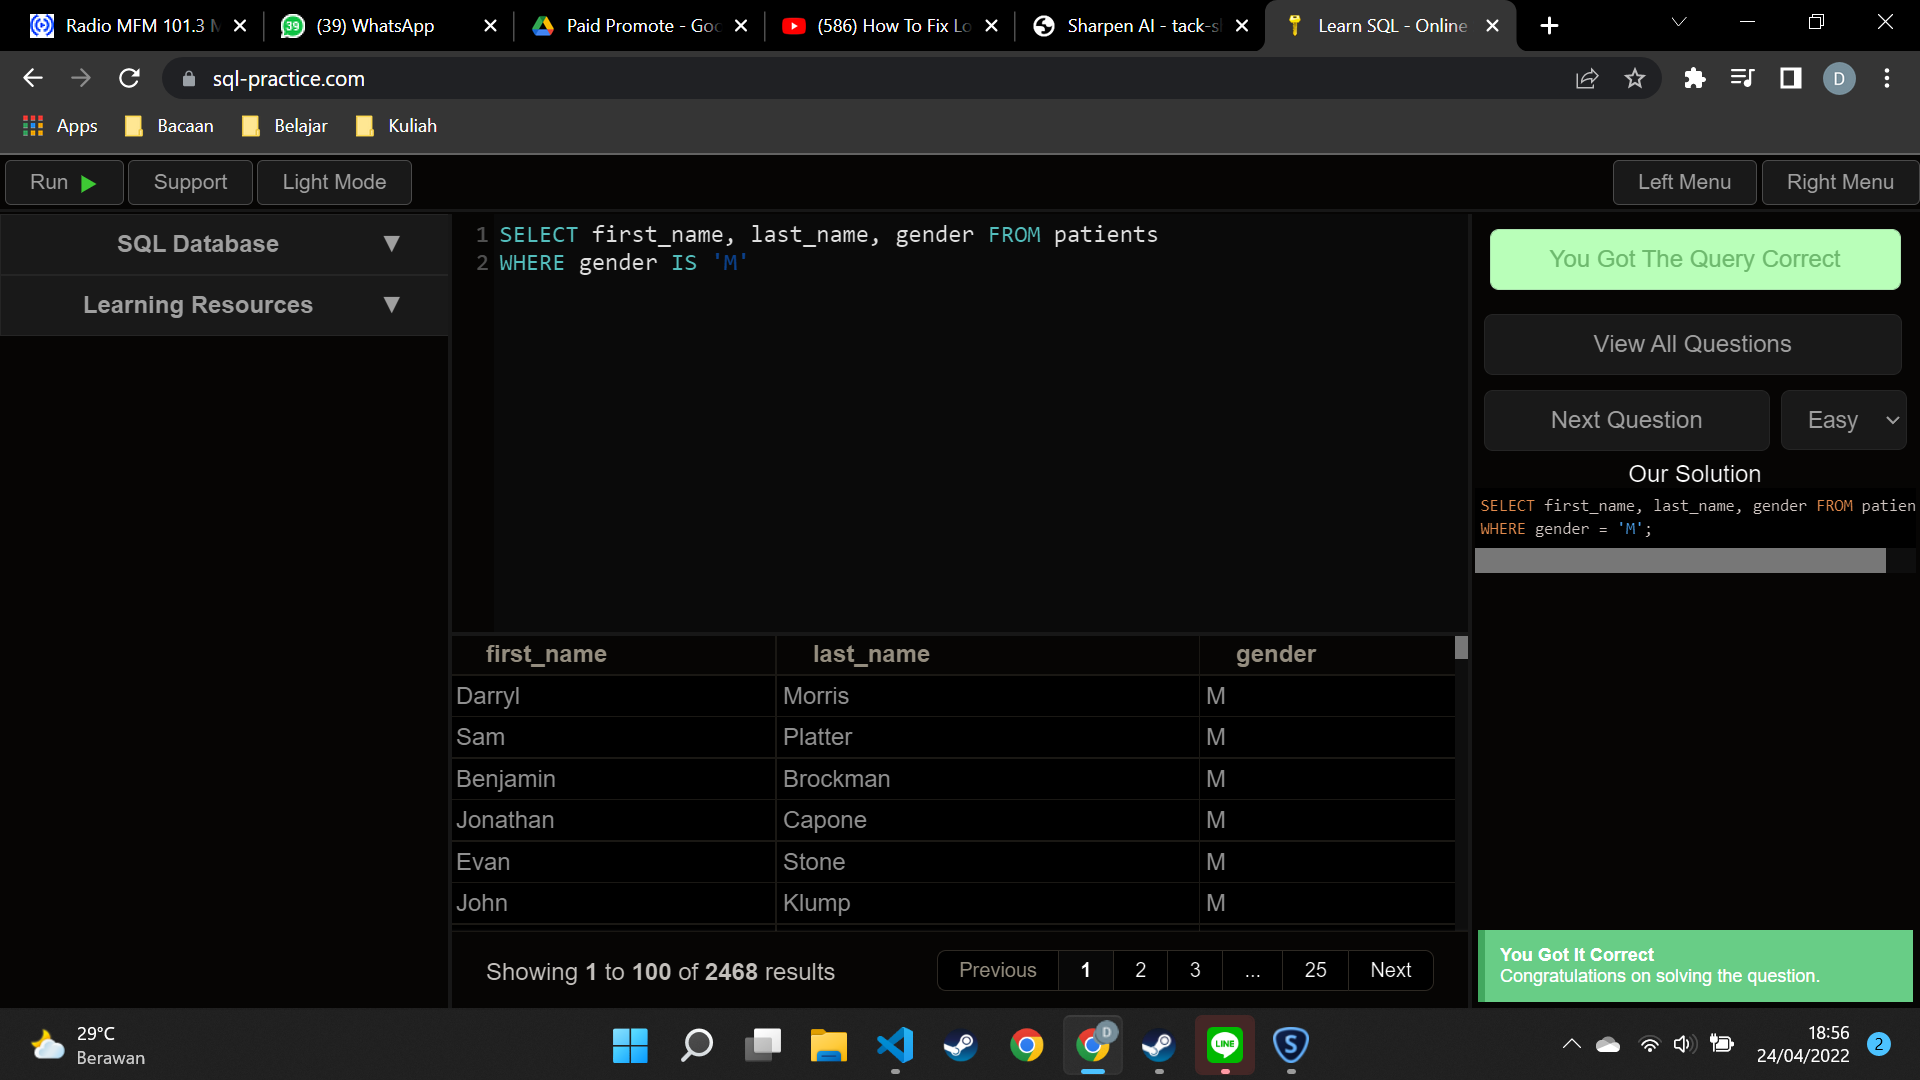
\includegraphics[scale=0.3]{./Screenshot/Easy-1.png}
            \centering
        \end{figure}

        \item Show first name and last name of patients who does not have allergies (null)
        \\Query :
        \lstinputlisting[label={listing2},caption={Easy - 2}, language={sql}]{"../Easy-2.sql"}
        \begin{itemize}
            \item Baris 1 : Mengambil data first\_name dan last\_name dari tabel patients
            \item Baris 2 : Dengan kondisi dimana allergies dari pasien bernilai null (tidak memiliki allergi)
        \end{itemize}
        Screenshot :
        \begin{figure}[h]
            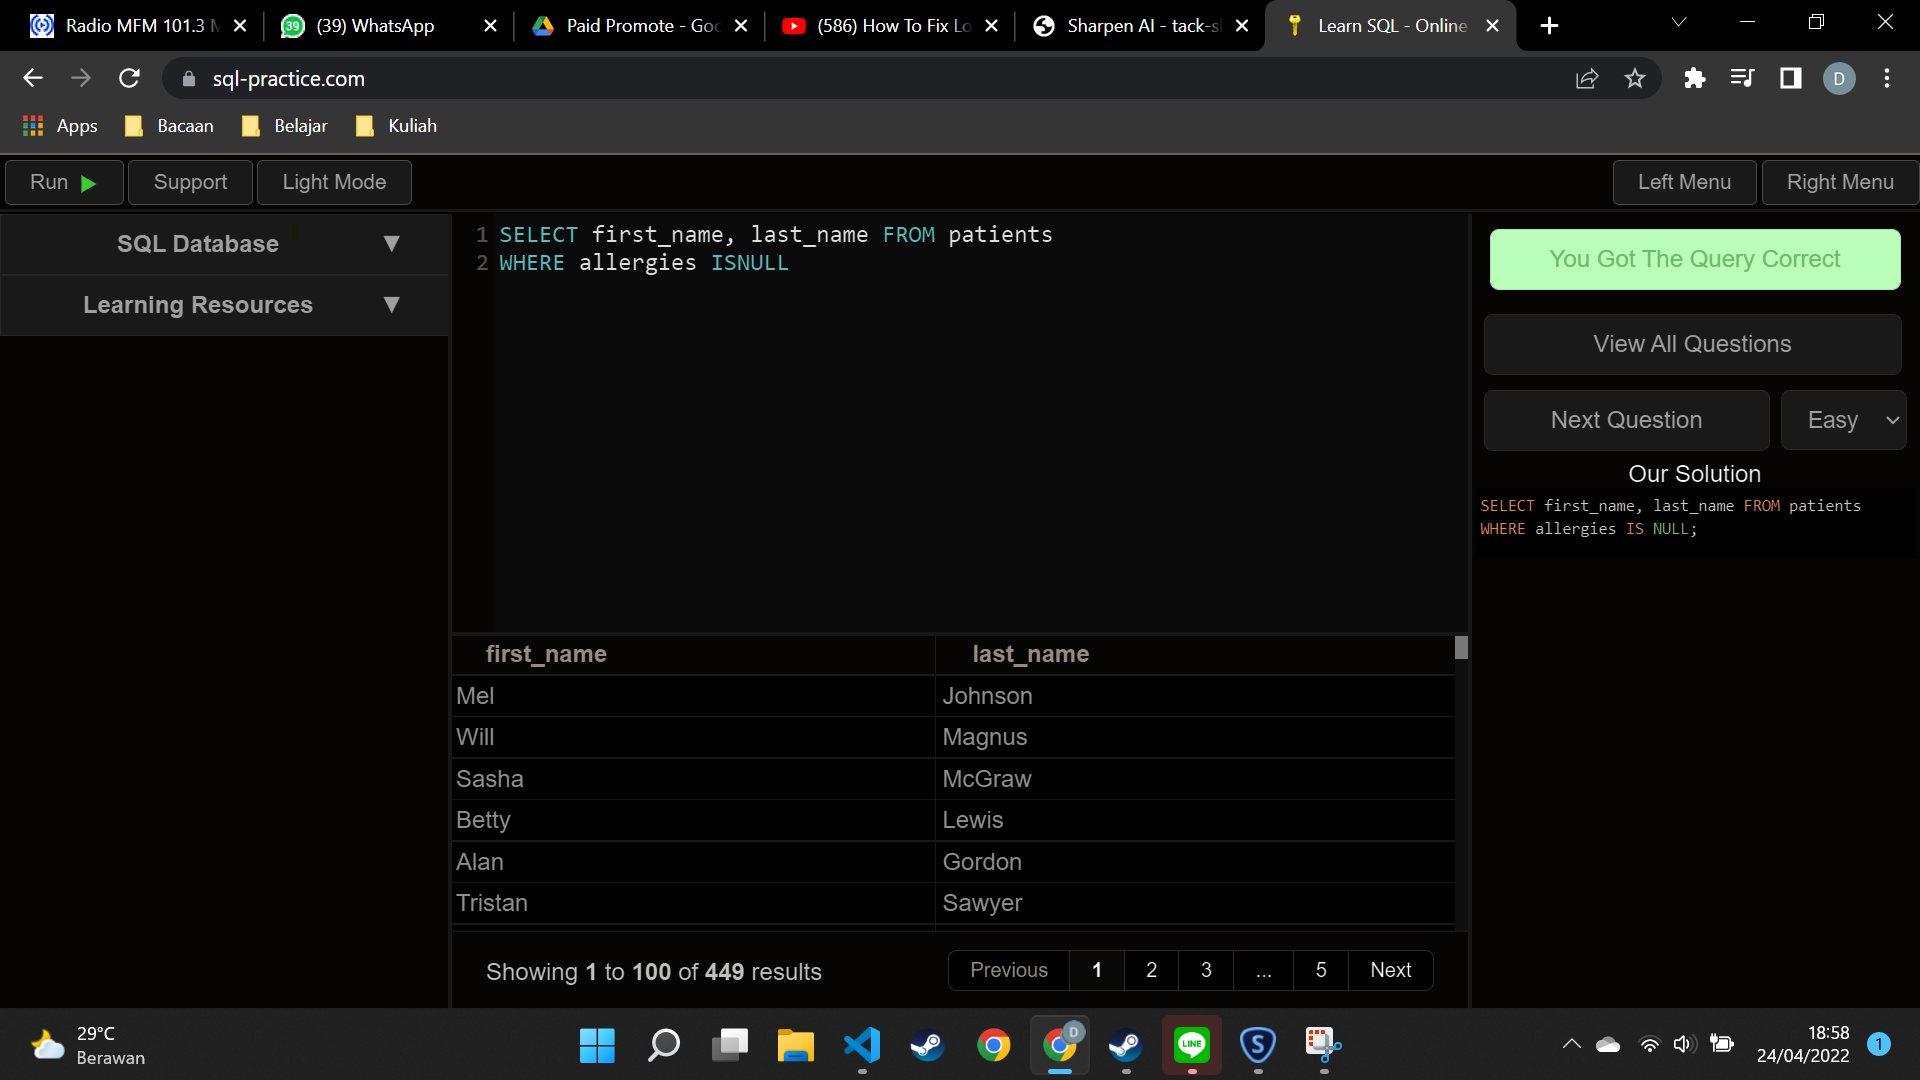
\includegraphics[scale=0.3]{./Screenshot/Easy-2.png}
            \centering
        \end{figure}

        \item Show first name of patients that start with the letter 'C'
        \\Query :
        \lstinputlisting[label={listing3},caption={Easy - 3}, language={sql}]{"../Easy-3.sql"}
        \begin{itemize}
            \item Baris 1 : Mengambil data first\_name dari tabel patients
            \item Baris 2 : Dengan kondisi dimana first\_name dari pasien diawali dengan huruf "C" 
        \end{itemize}
        \pagebreak
        Screenshot :
        \begin{figure}[h]
            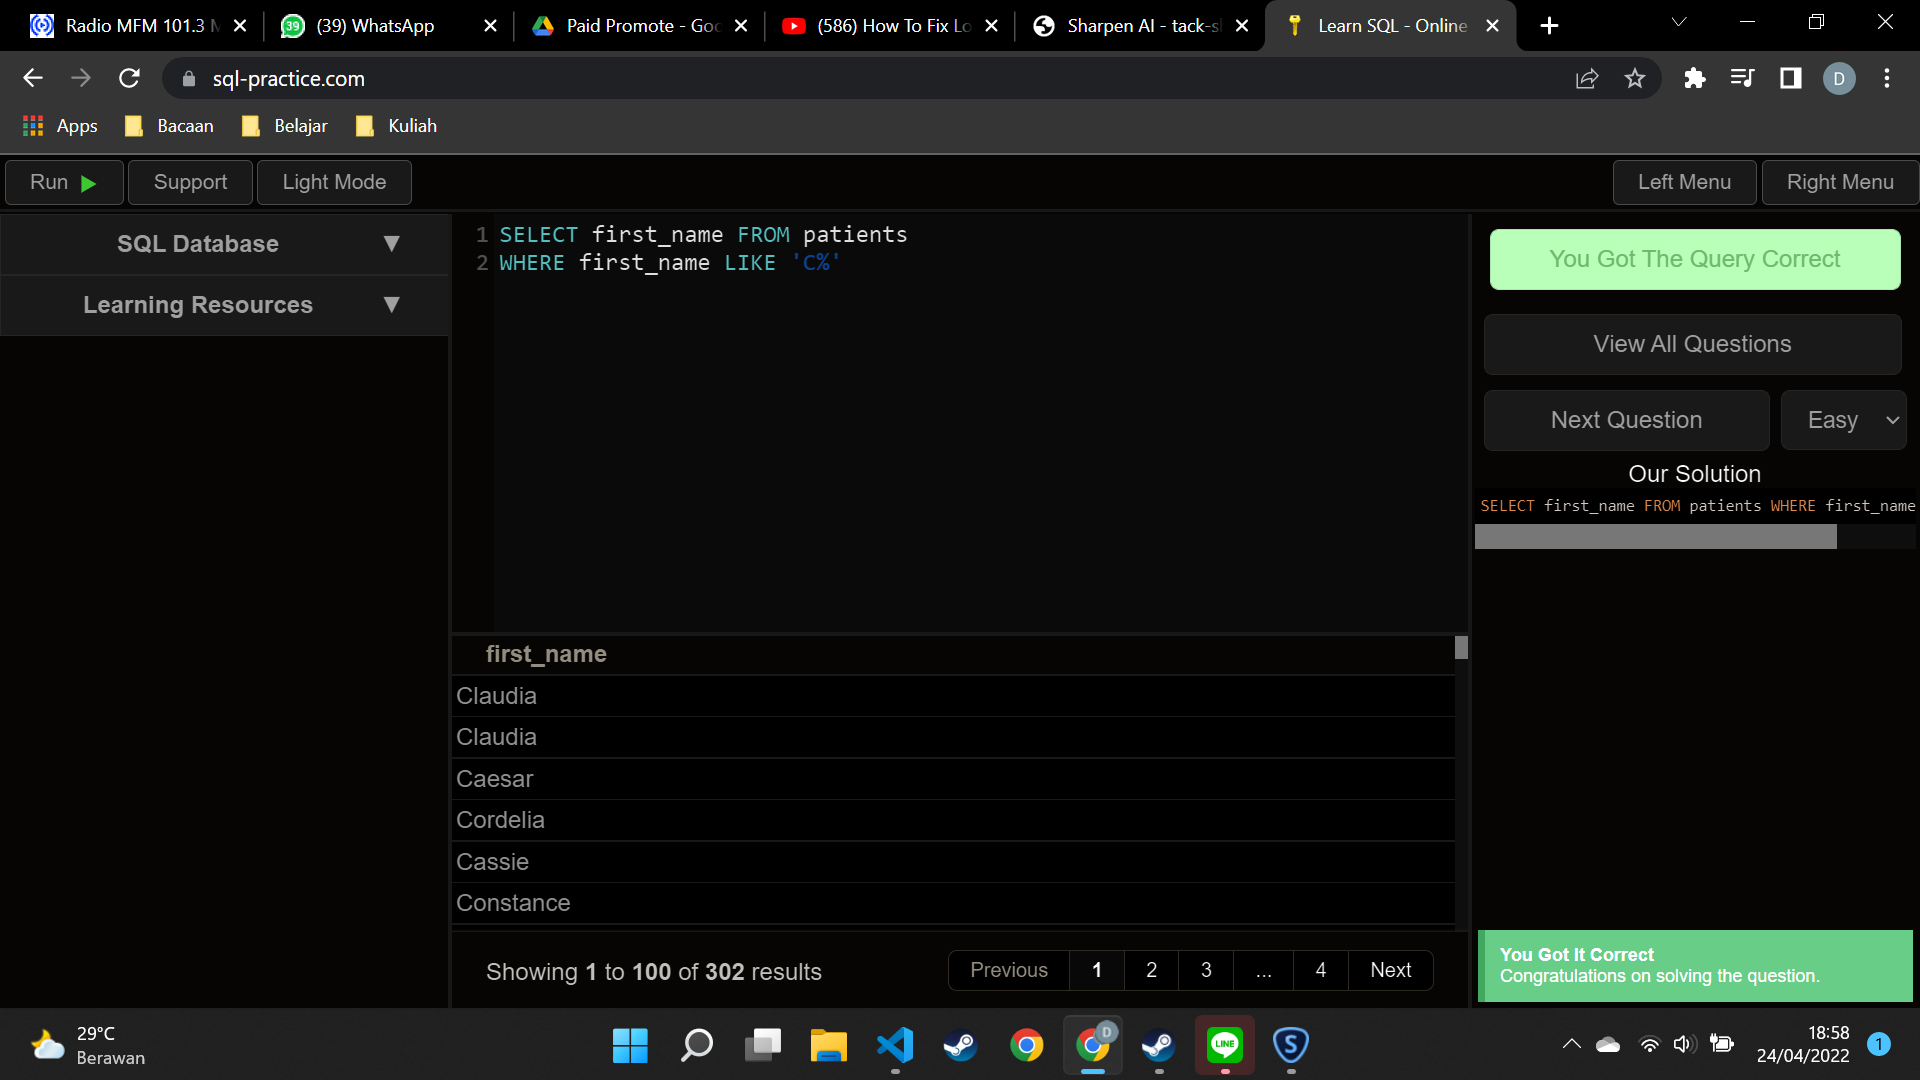
\includegraphics[scale=0.3]{./Screenshot/Easy-3.png}
            \centering
        \end{figure}

        \item Show first name and last name of patients that weight within the range of 100 to 120 (inclusive)
        \\Query :
        \lstinputlisting[label={listing4},caption={Easy - 4}, language={sql}]{"../Easy-4.sql"}
        \begin{itemize}
            \item Baris 1 : Mengambil data first\_name dan last\_name dari tabel patients
            \item Baris 2 : Dengan kondisi dimana weight dari pasien bernilai diantara 100 dan 120
        \end{itemize}
        Screenshot :
        \begin{figure}[h]
            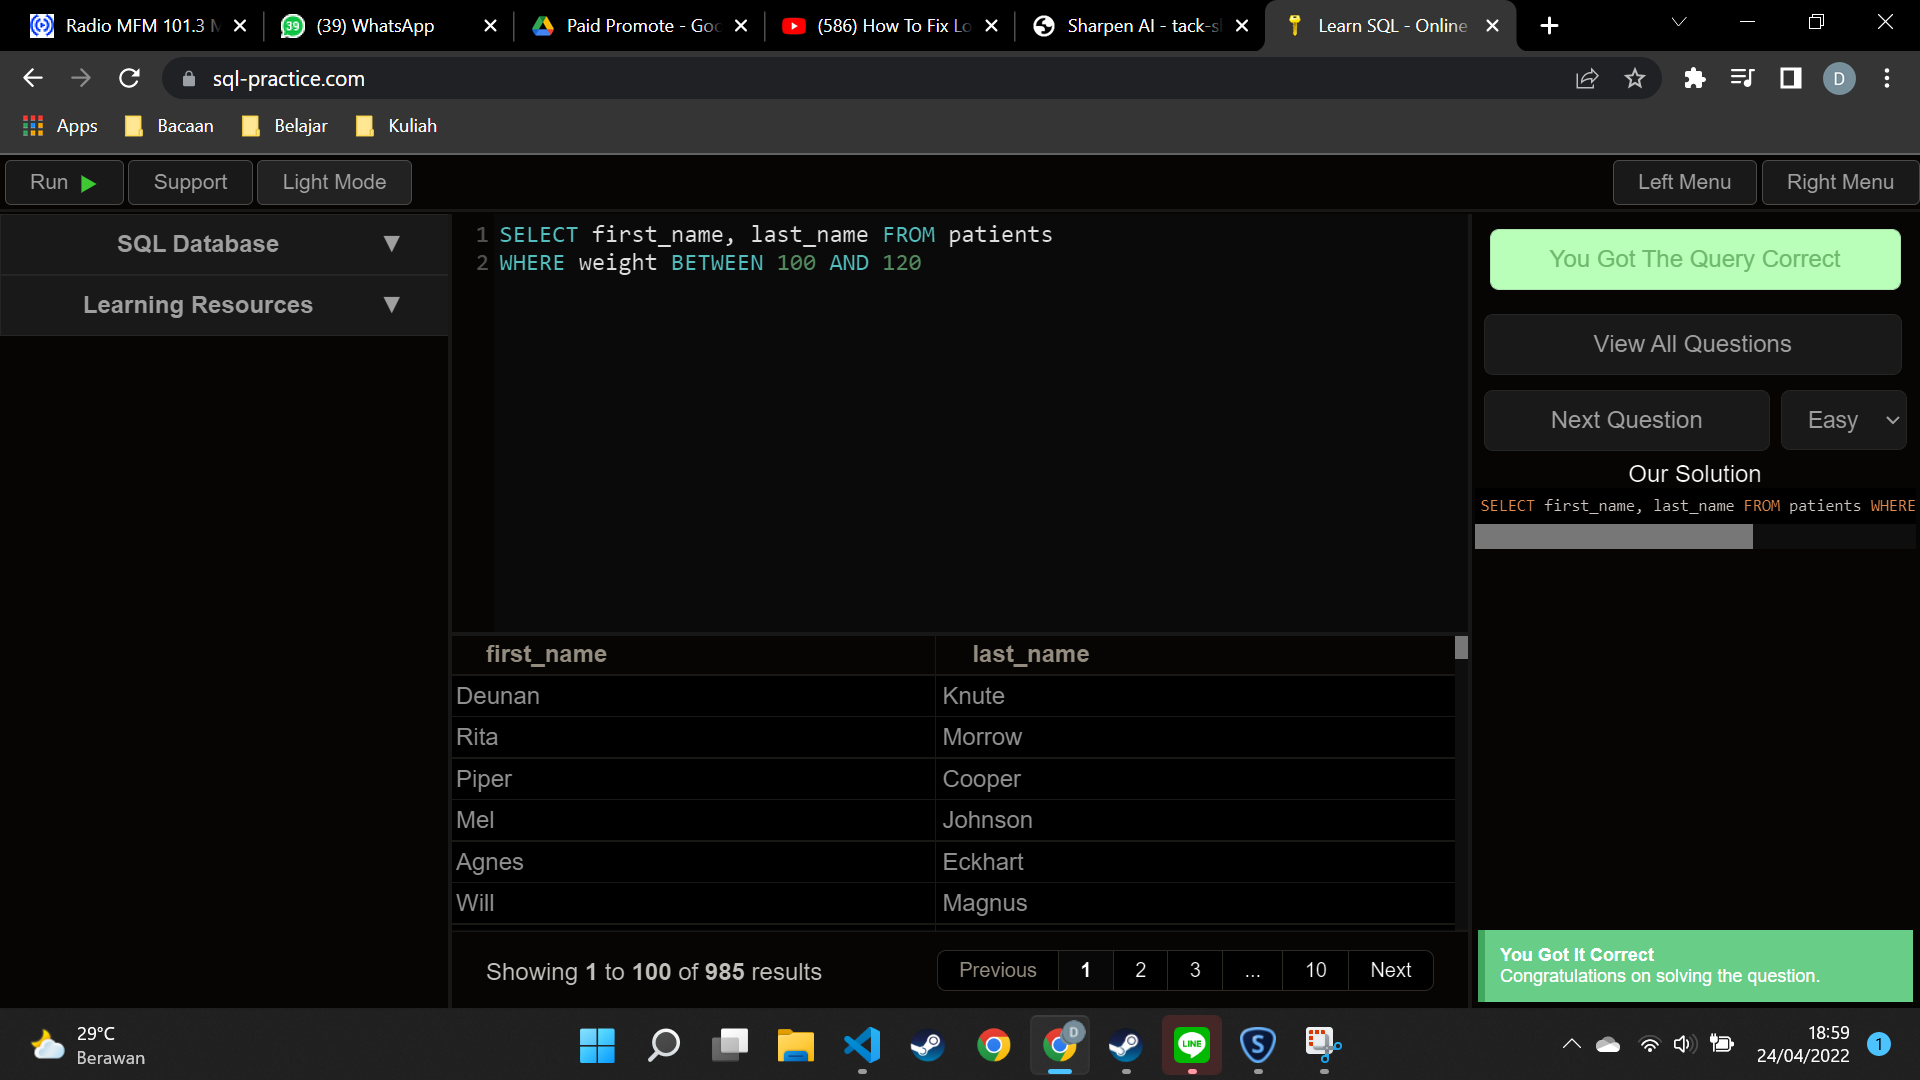
\includegraphics[scale=0.3]{./Screenshot/Easy-4.png}
            \centering
        \end{figure}

        \item Update the patients table for the allergies column. If the patient's allergies is null then replace it with 'NKA'
        \\Query :
        \lstinputlisting[label={listing5},caption={Easy - 5}, language={sql}]{"../Easy-5.sql"}
        \begin{itemize}
            \item Baris 1 : Mengupdate tabel patients
            \item Baris 2 : Kolom allergies akan diisi dengan "NKA"
            \item Baris 3 : Pada data dimana allergies dari pasien bernilai null (tidak memiliki allergi)
        \end{itemize}
        Screenshot :
        \begin{figure}[h]
            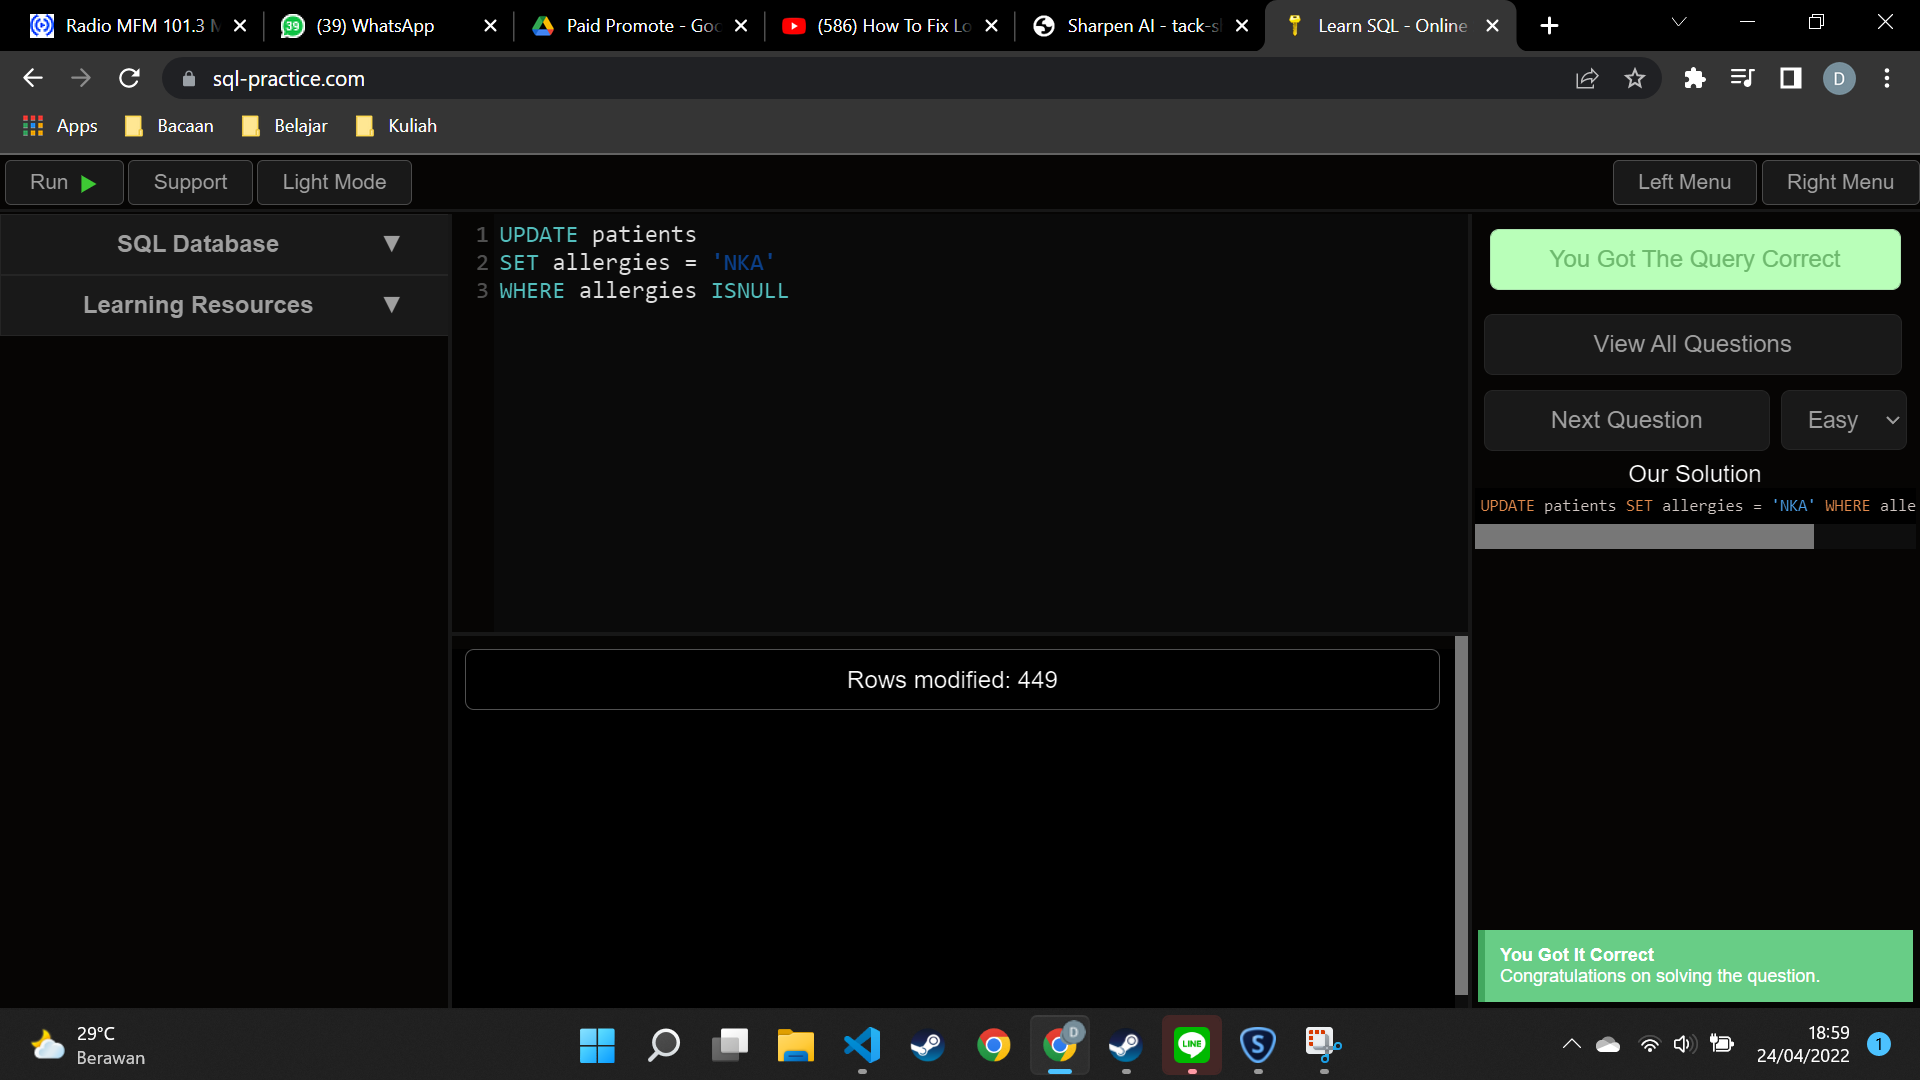
\includegraphics[scale=0.3]{./Screenshot/Easy-5.png}
            \centering
        \end{figure}

        \item Show first name and last name concatinated into one column to show their full name
        \\Query :
        \lstinputlisting[label={listing6},caption={Easy - 6}, language={sql}]{"../Easy-6.sql"}
        \begin{itemize}
            \item Baris 1 : Mengambil data gabungan dari first\_name dan last\_name yang akan disebut sebagai full\_name dari data pada tabel patients
        \end{itemize}
        \pagebreak
        Screenshot :
        \begin{figure}[h]
            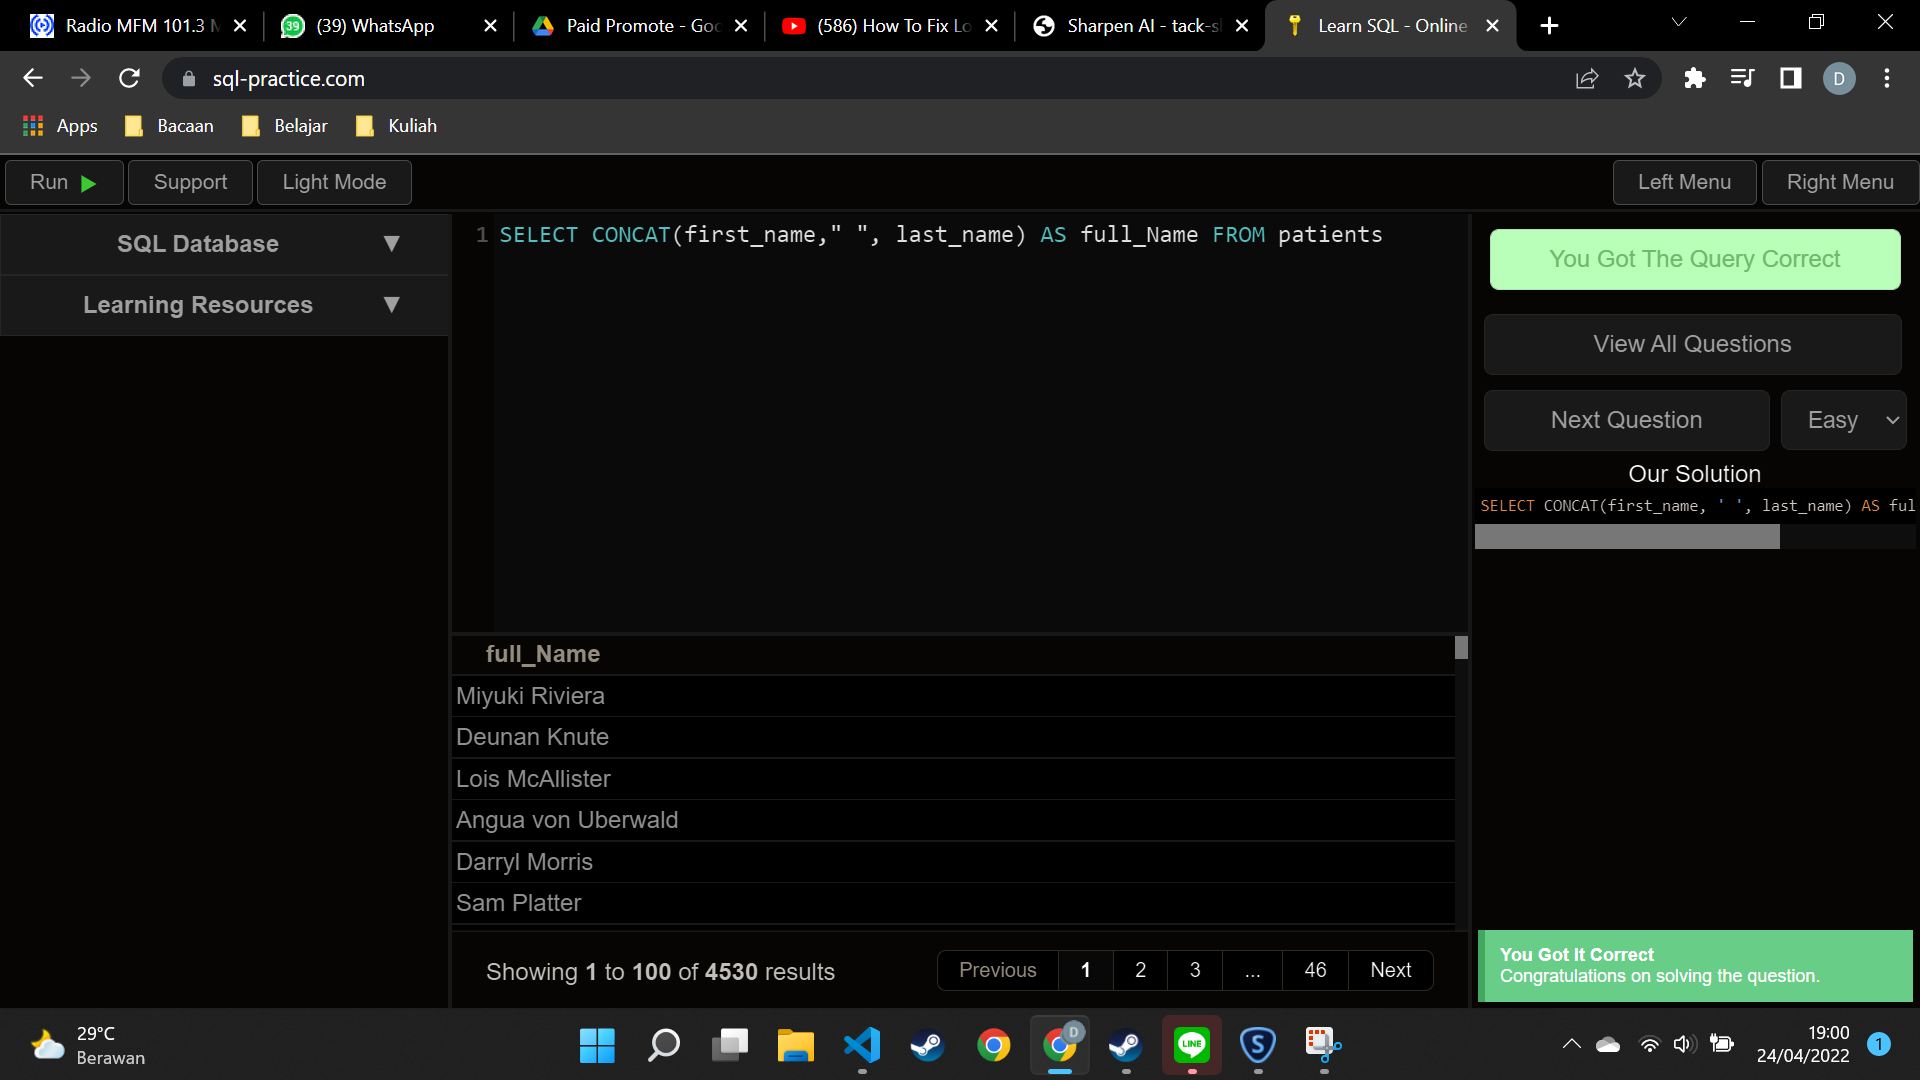
\includegraphics[scale=0.3]{./Screenshot/Easy-6.png}
            \centering
        \end{figure}

        \item Show first name, last name, and the full province name of each patient. Example: 'Ontario' instead of 'ON'
        \\Query :
        \lstinputlisting[label={listing7},caption={Easy - 7}, language={sql}]{"../Easy-7.sql"}
        \begin{itemize}
            \item Baris 1 : Mengambil data first\_name, last\_name, dan provincename dari tabel patients
            \item Baris 2 : Menggabungkan tabel provinces sesuai dengan data tabel patients
            \item Baris 3 : Dengan acuan province\_id pada tabel patients merujuk pada province\_id pada tabel provinces
        \end{itemize}
        \pagebreak
        Screenshot :
        \begin{figure}[h]
            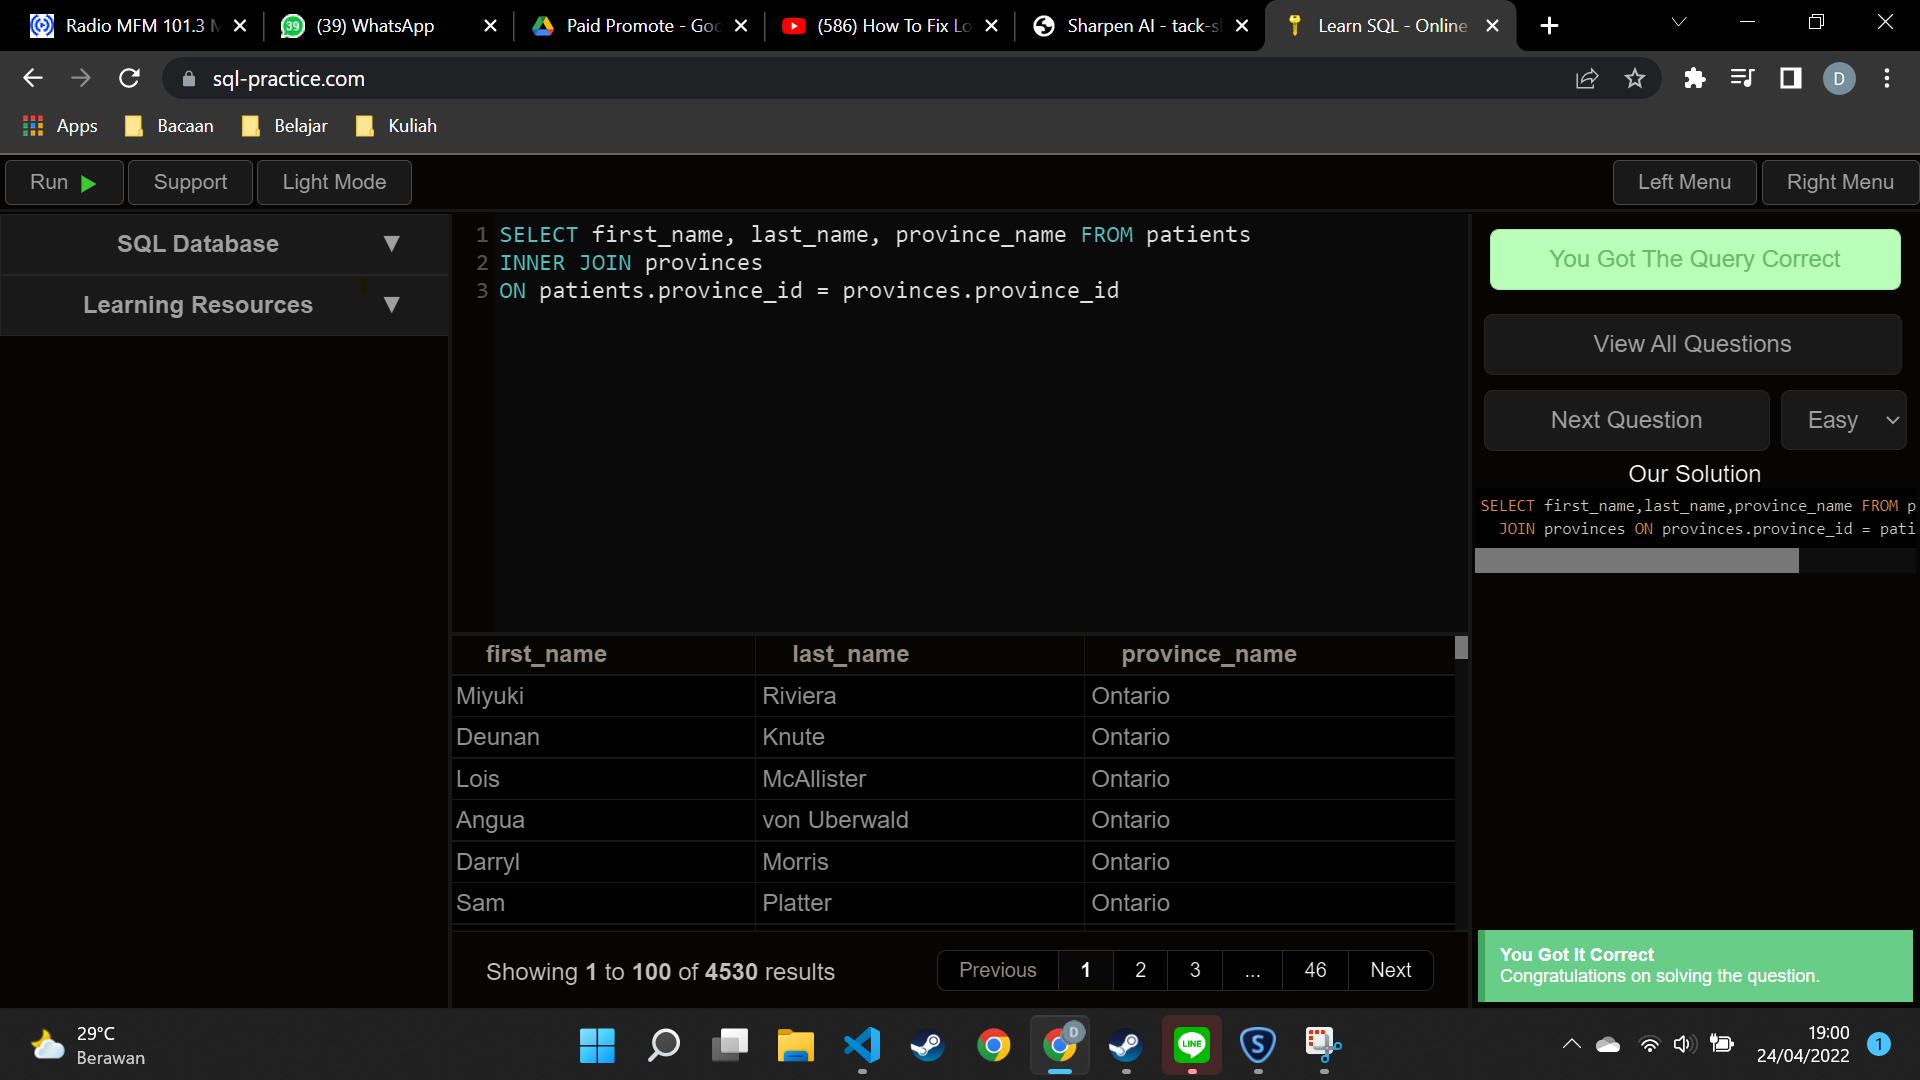
\includegraphics[scale=0.3]{./Screenshot/Easy-7.png}
            \centering
        \end{figure}

        \item Show how many patients have a birth\_date with 2010 as the birth year
        \\Query :
        \lstinputlisting[label={listing8},caption={Easy - 8}, language={sql}]{"../Easy-8.sql"}
        \begin{itemize}
            \item Baris 1 : Mengambil banyaknya data pada kolom brthdate dari tabel patients
            \item Baris 2 : Dengan kondisi dimana tahun birth\_date dari pasien adalah 2010
        \end{itemize}
        Screenshot :
        \begin{figure}[h]
            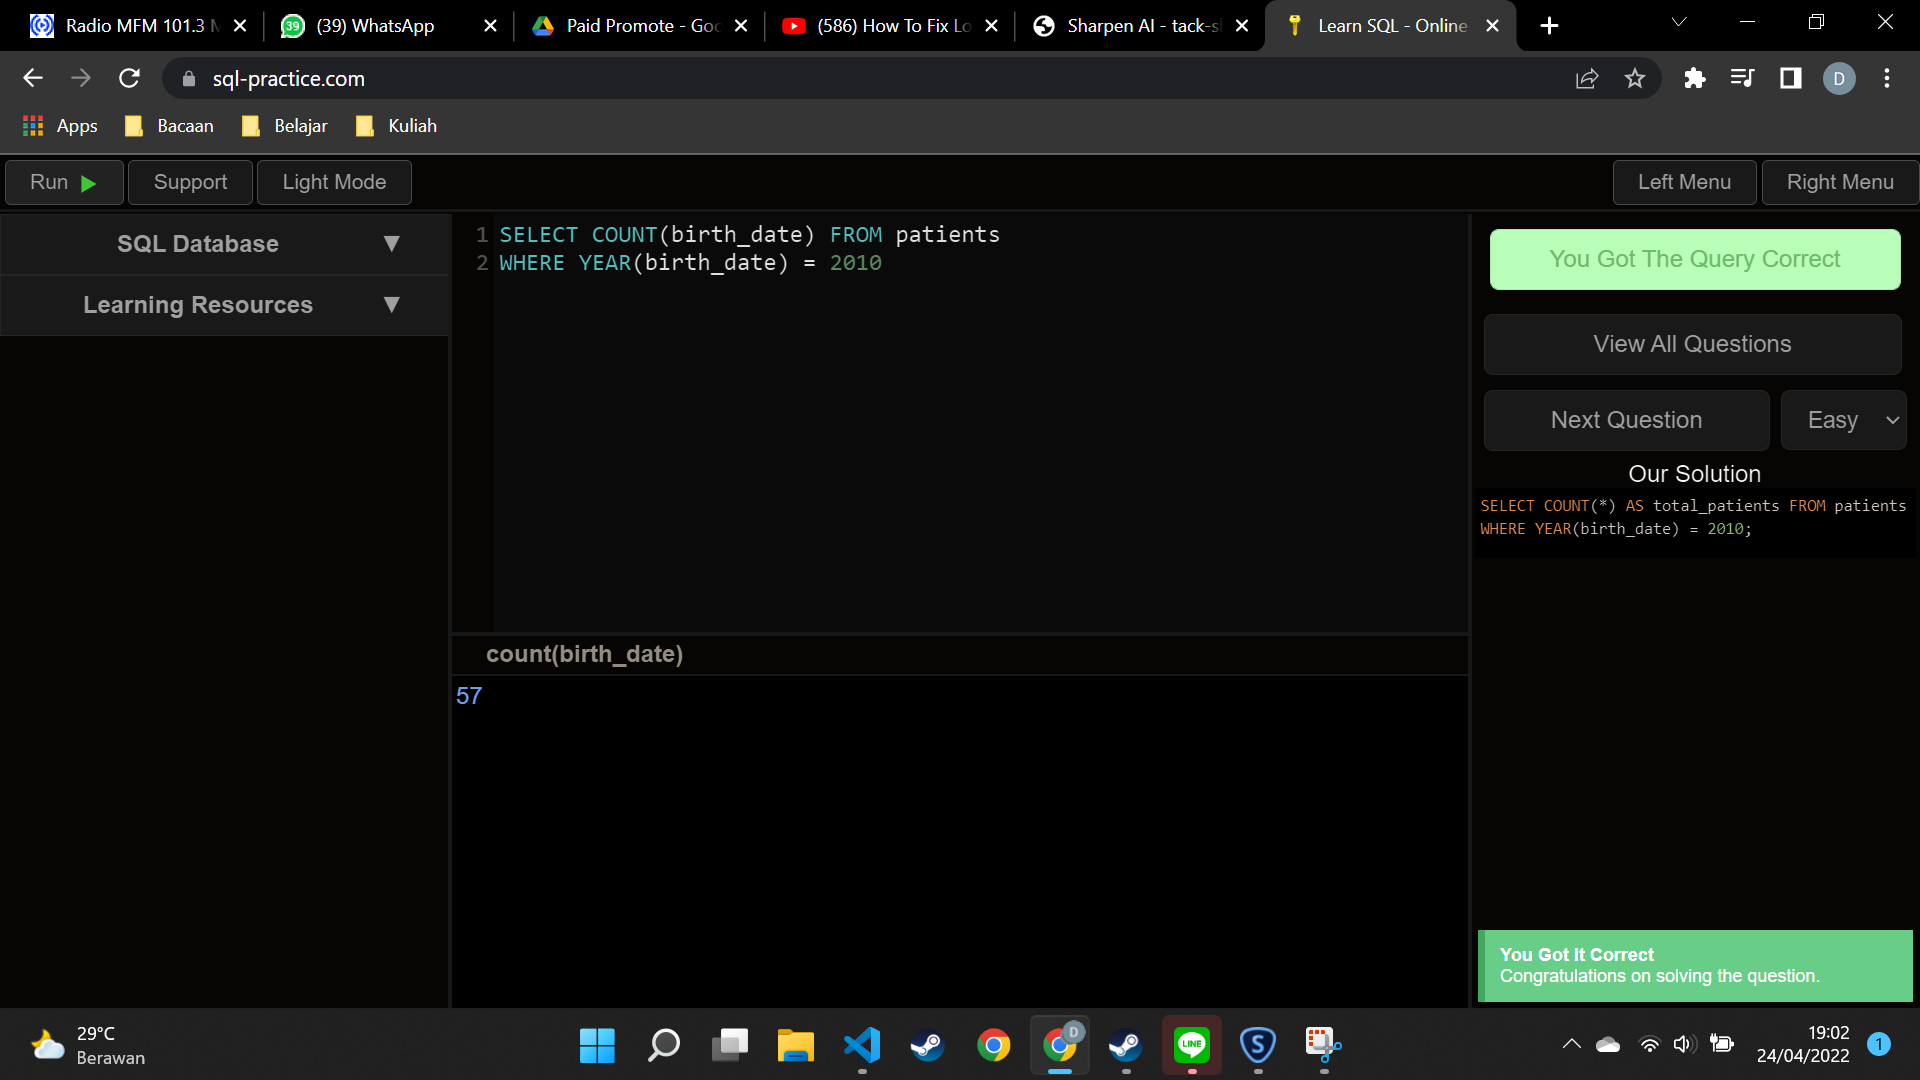
\includegraphics[scale=0.3]{./Screenshot/Easy-8.png}
            \centering
        \end{figure}

        \item Show the first\_name, last\_name, and height of the patient with the greatest height
        \\Query :
        \lstinputlisting[label={listing9},caption={Easy - 9}, language={sql}]{"../Easy-9.sql"}
        \begin{itemize}
            \item Baris 1 : Mengambil data first\_name, last\_name, dan height dari tabel patients
            \item Baris 2 : Mengurutkan data berdasarkan height secara descending (dari height terbesar), dan ambil 1 data pertama
        \end{itemize}
        Screenshot :
        \begin{figure}[h]
            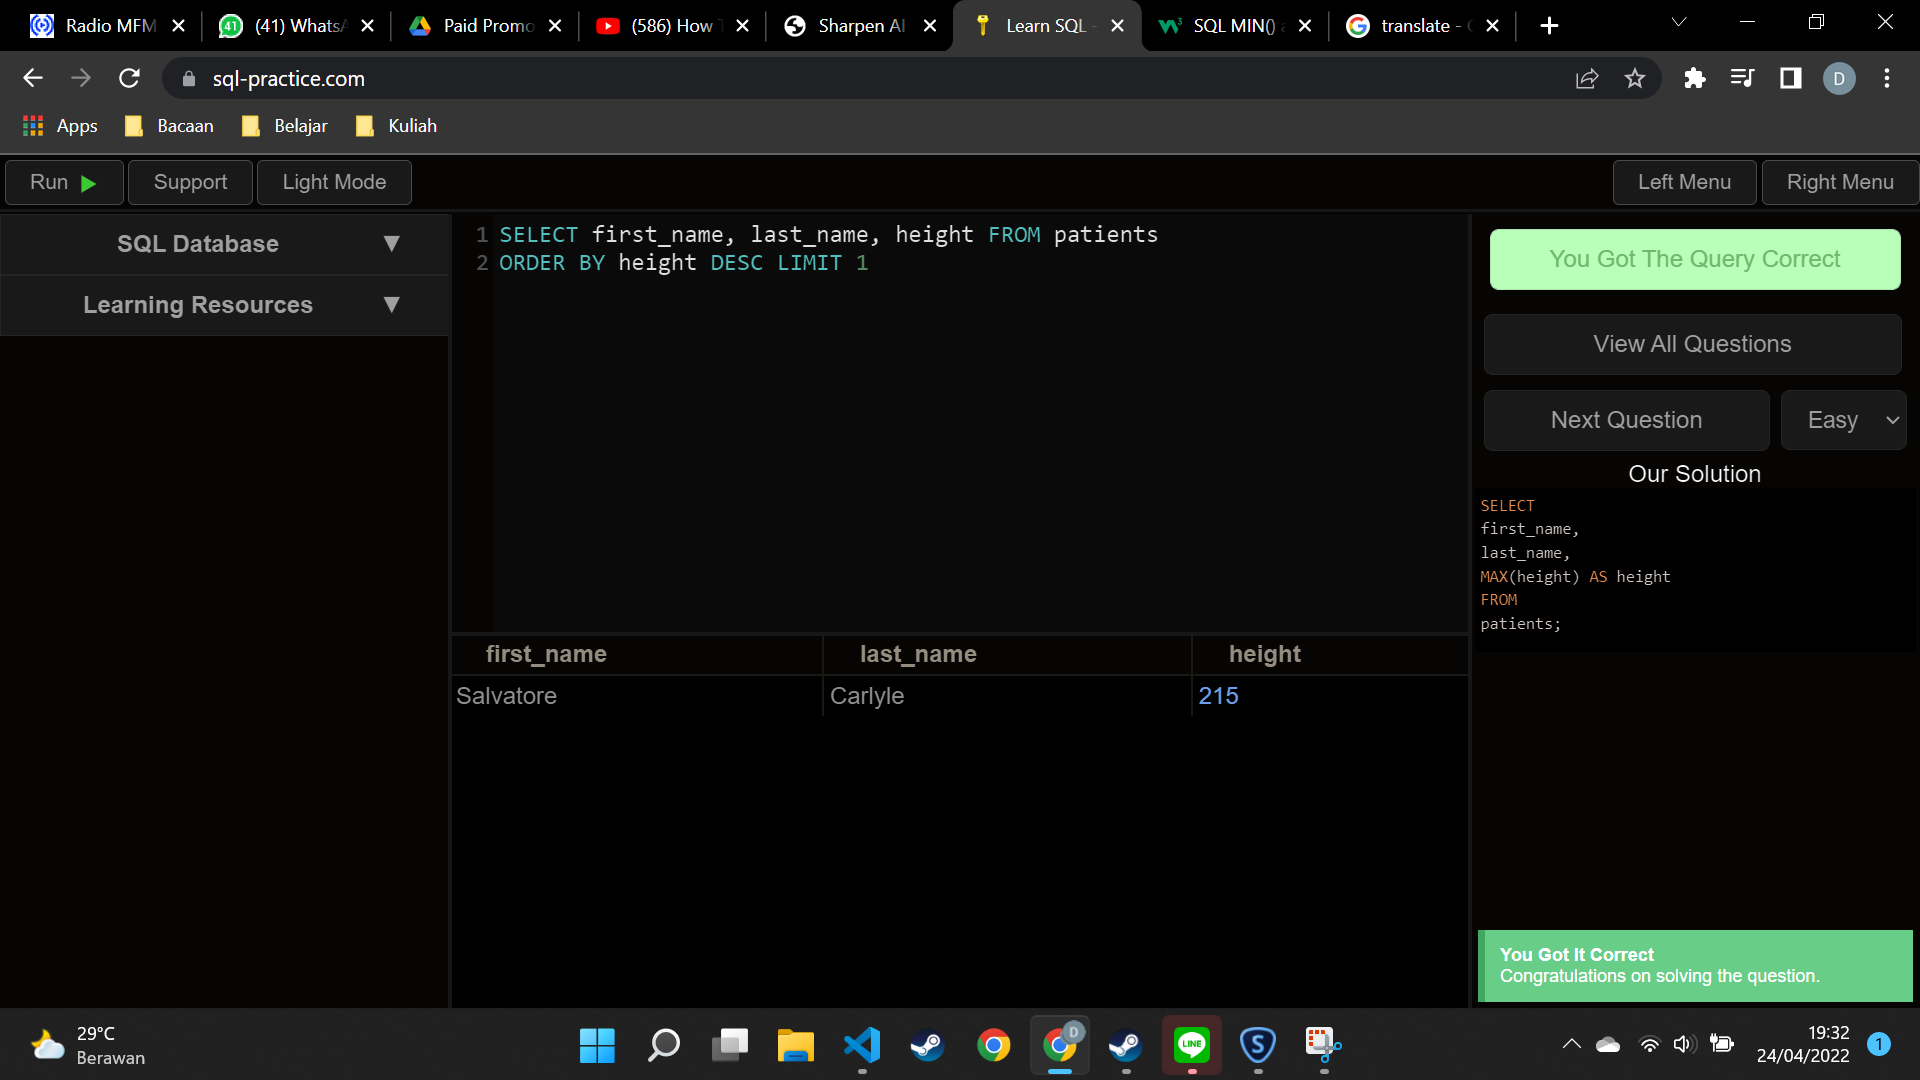
\includegraphics[scale=0.3]{./Screenshot/Easy-9.png}
            \centering
        \end{figure}

        \item Show all columns for patients who have one of the following patient\_ids: 1,45,534,879,1000
        \\Query :
        \lstinputlisting[label={listing10},caption={Easy - 10}, language={sql}]{"../Easy-10.sql"}
        \begin{itemize}
            \item Baris 1 : Mengambil semua data dari tabel patients
            \item Baris 2 : Dengan kondisi dimana patient\_id nya termasuk diantara 1, 45, 534, 879, 1000
        \end{itemize}
        \pagebreak
        Screenshot :
        \begin{figure}[h]
            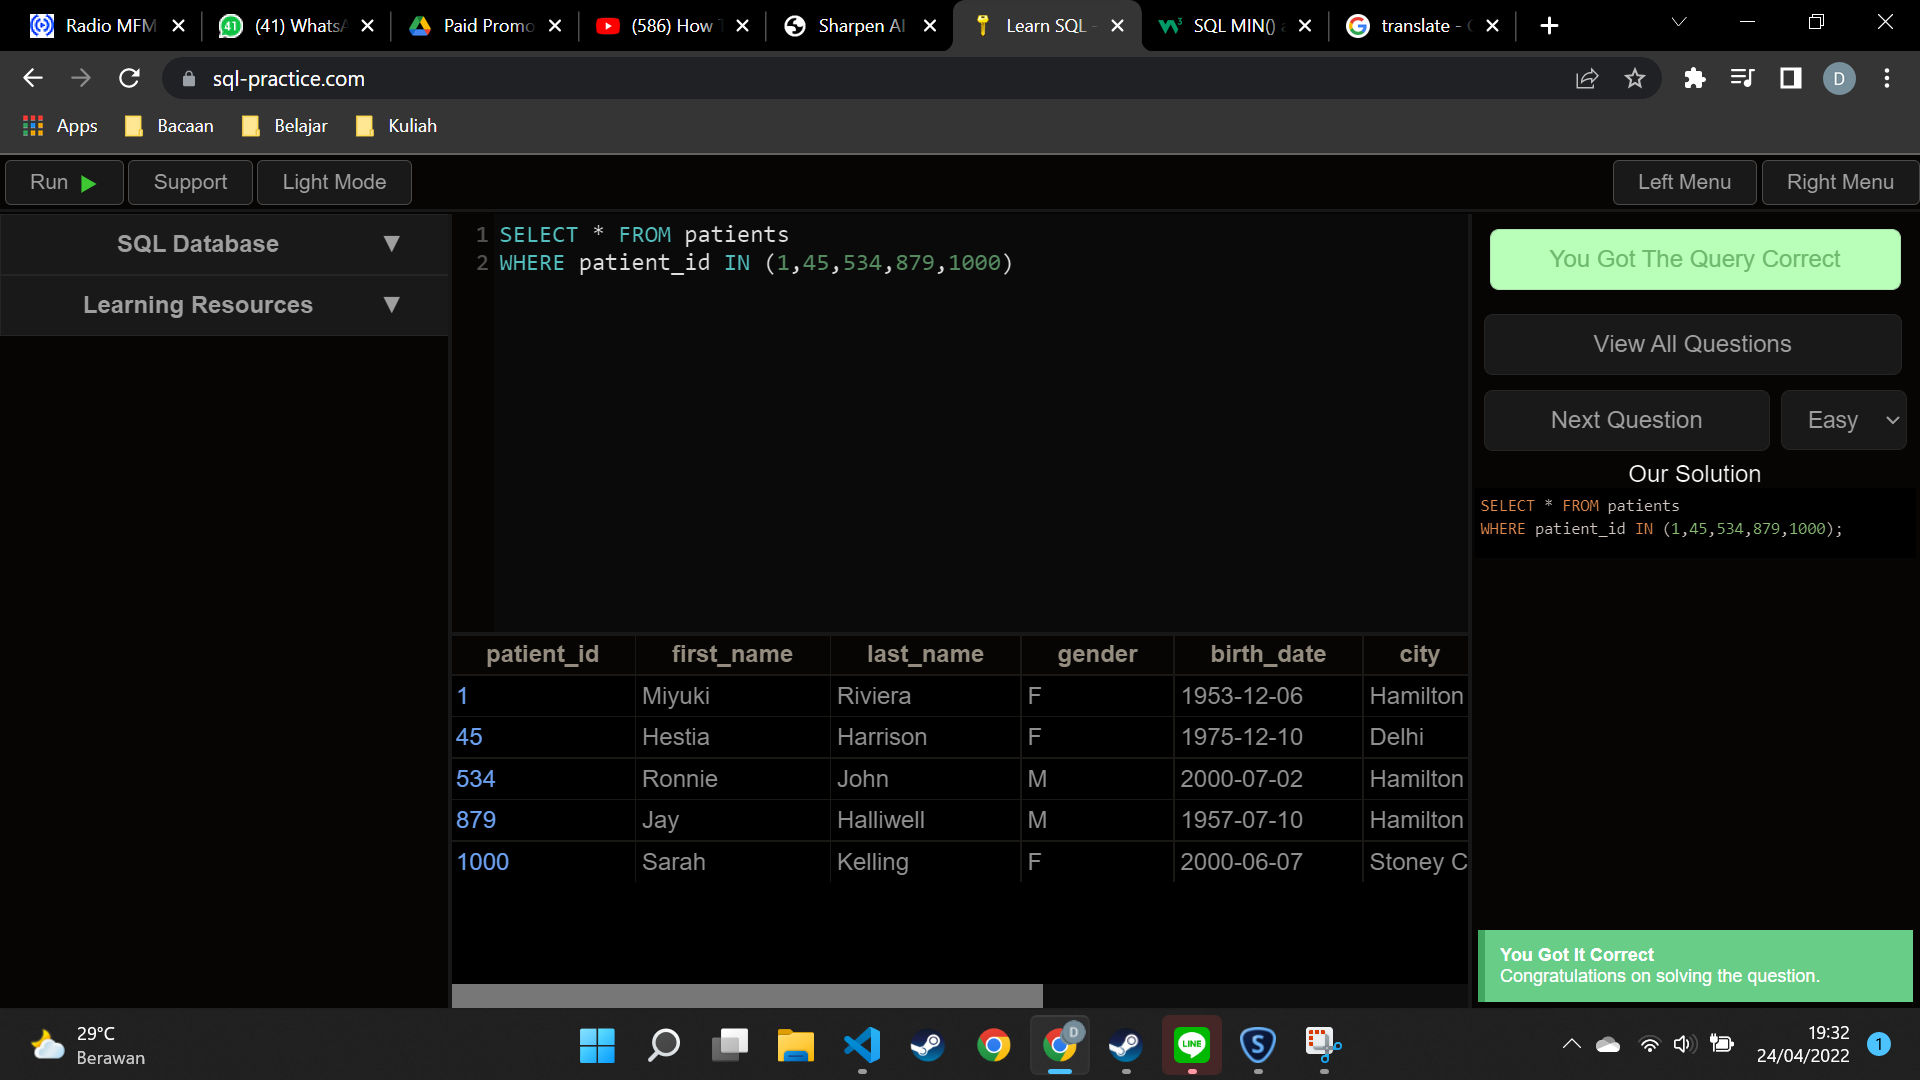
\includegraphics[scale=0.3]{./Screenshot/Easy-10.png}
            \centering
        \end{figure}

        \item Show the total number of admissions
        \\Query :
        \lstinputlisting[label={listing11},caption={Easy - 11}, language={sql}]{"../Easy-11.sql"}
        \begin{itemize}
            \item Baris 1 : Mengambil banyaknya data dari admissions (akan disebut sebagai total\_admissions)
        \end{itemize}
        Screenshot :
        \begin{figure}[h]
            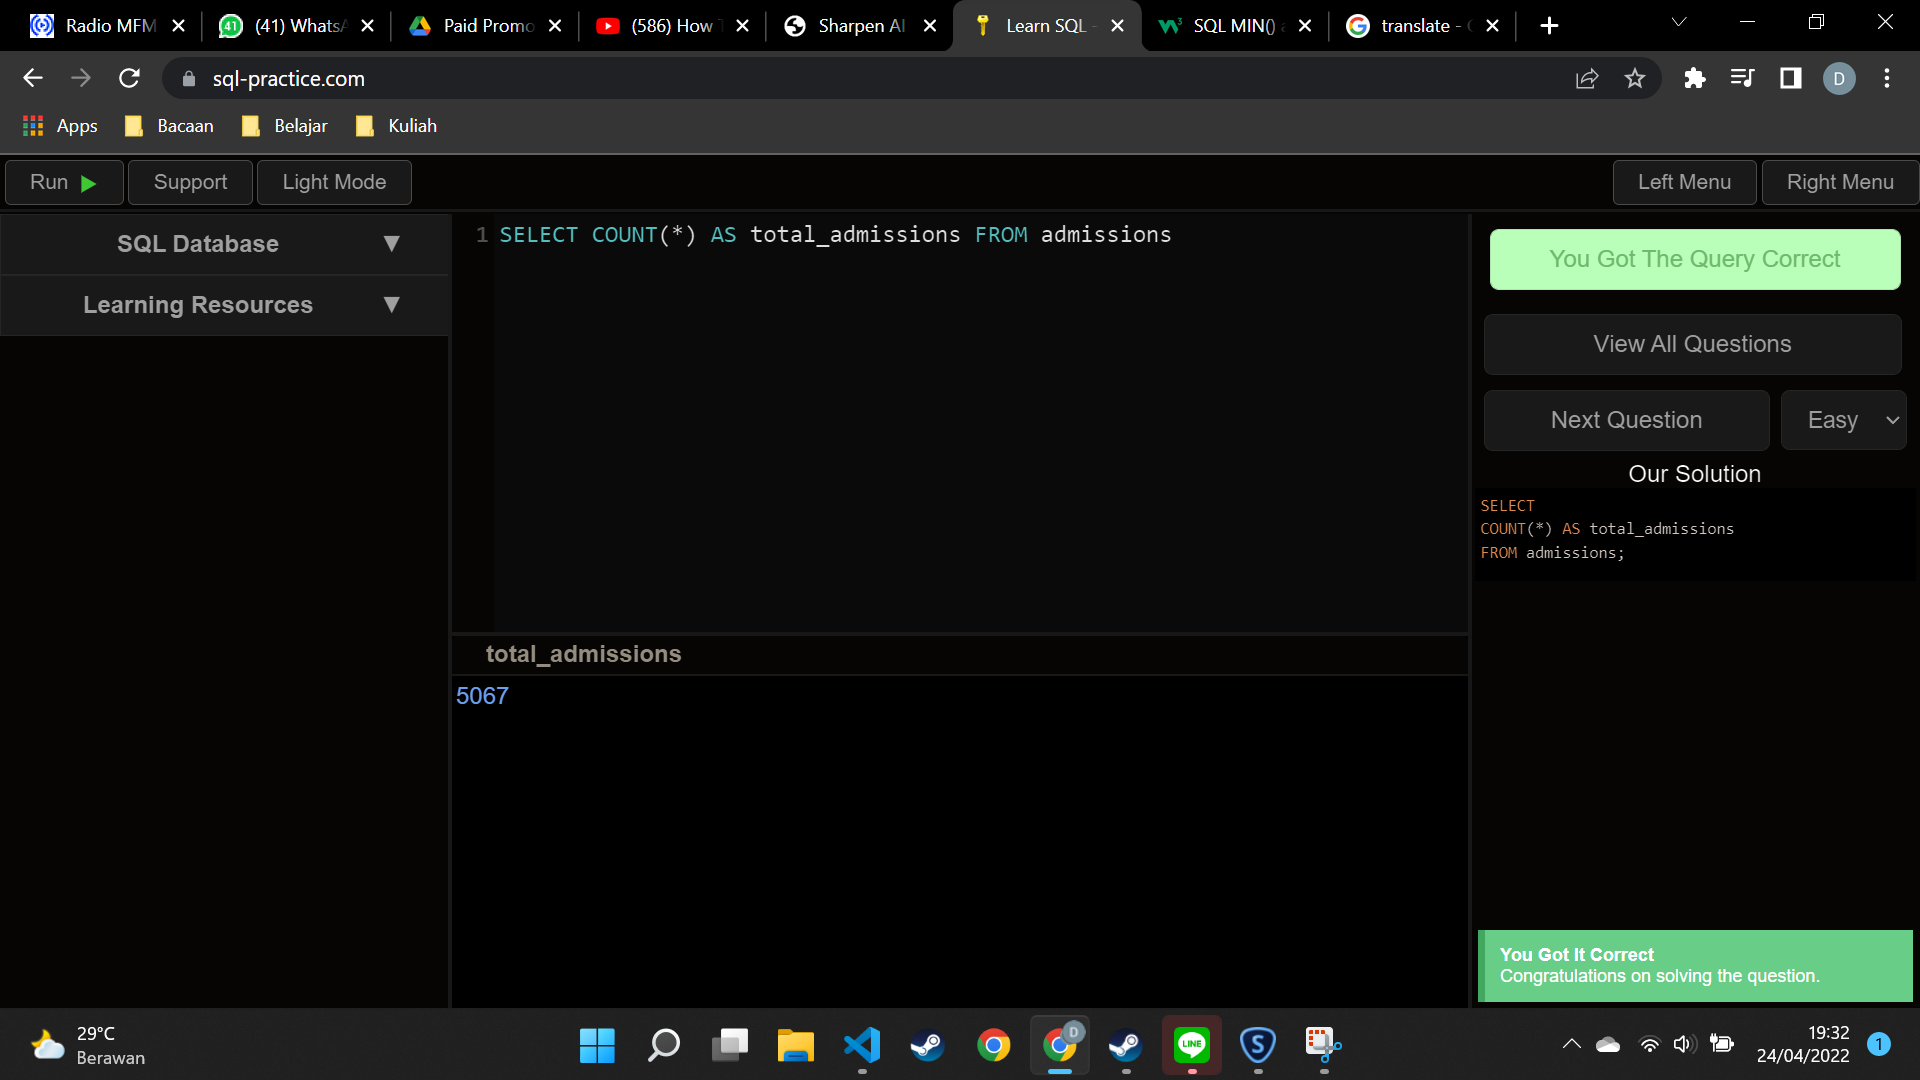
\includegraphics[scale=0.3]{./Screenshot/Easy-11.png}
            \centering
        \end{figure}

    \end{itemize}

\section{Soal Medium}
    \begin{itemize}
        \item Show unique birth years from patients and order them by ascending
        \\Query : 
        \lstinputlisting[label={listing12},caption={Medium - 1}, language={sql}]{"../Medium-1.sql"}
        Penjelasan :
        \begin{itemize}
            \item Baris 1 : Mengambil data tahun yang unik (distinct) pada kolom birth\_date dari tabel patients 
            \item Baris 2 : Mengurutkan secara ascending berdasarkan birth\_date
        \end{itemize}
        Screenshot :
        \begin{figure}[h]
            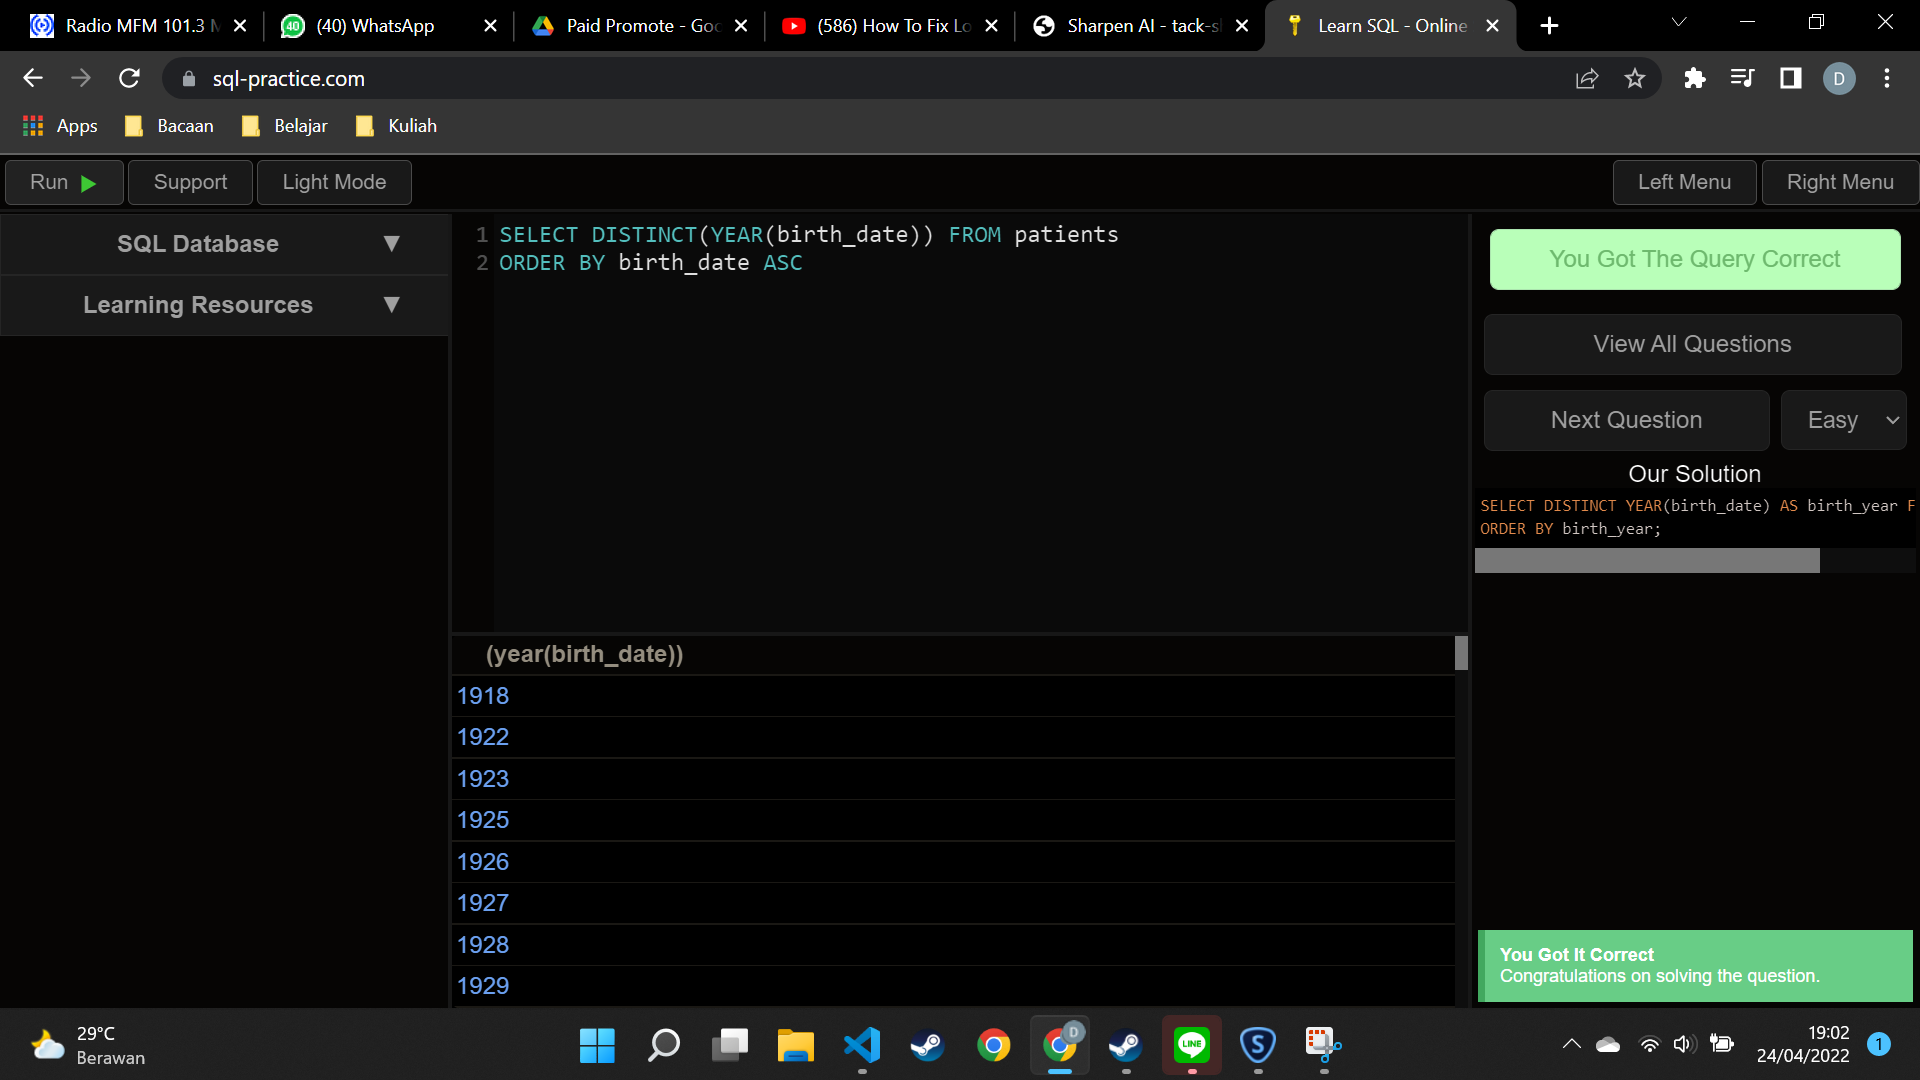
\includegraphics[scale=0.3]{./Screenshot/Medium-1.png}
            \centering
        \end{figure}

        \item Show unique first names from the patients table which only occurs once in the list. For example, if two or more people are named 'John' in the first\_name column then don't include their name in the output list. If only 1 person is named 'Leo' then include them in the output.
        \\Query :
        \lstinputlisting[label={listing13},caption={Medium - 2}, language={sql}]{"../Medium-2.sql"}
        \begin{itemize}
            \item Baris 1 : Mengambil data first\_name dari tabel patients
            \item Baris 2 : Mengelompokkan data berdasarkan first\_name
            \item Baris 3 : Mengambil data dengan jumlah data dalam kelompok adalah 1
        \end{itemize}
        \pagebreak
        Screenshot :
        \begin{figure}[h]
            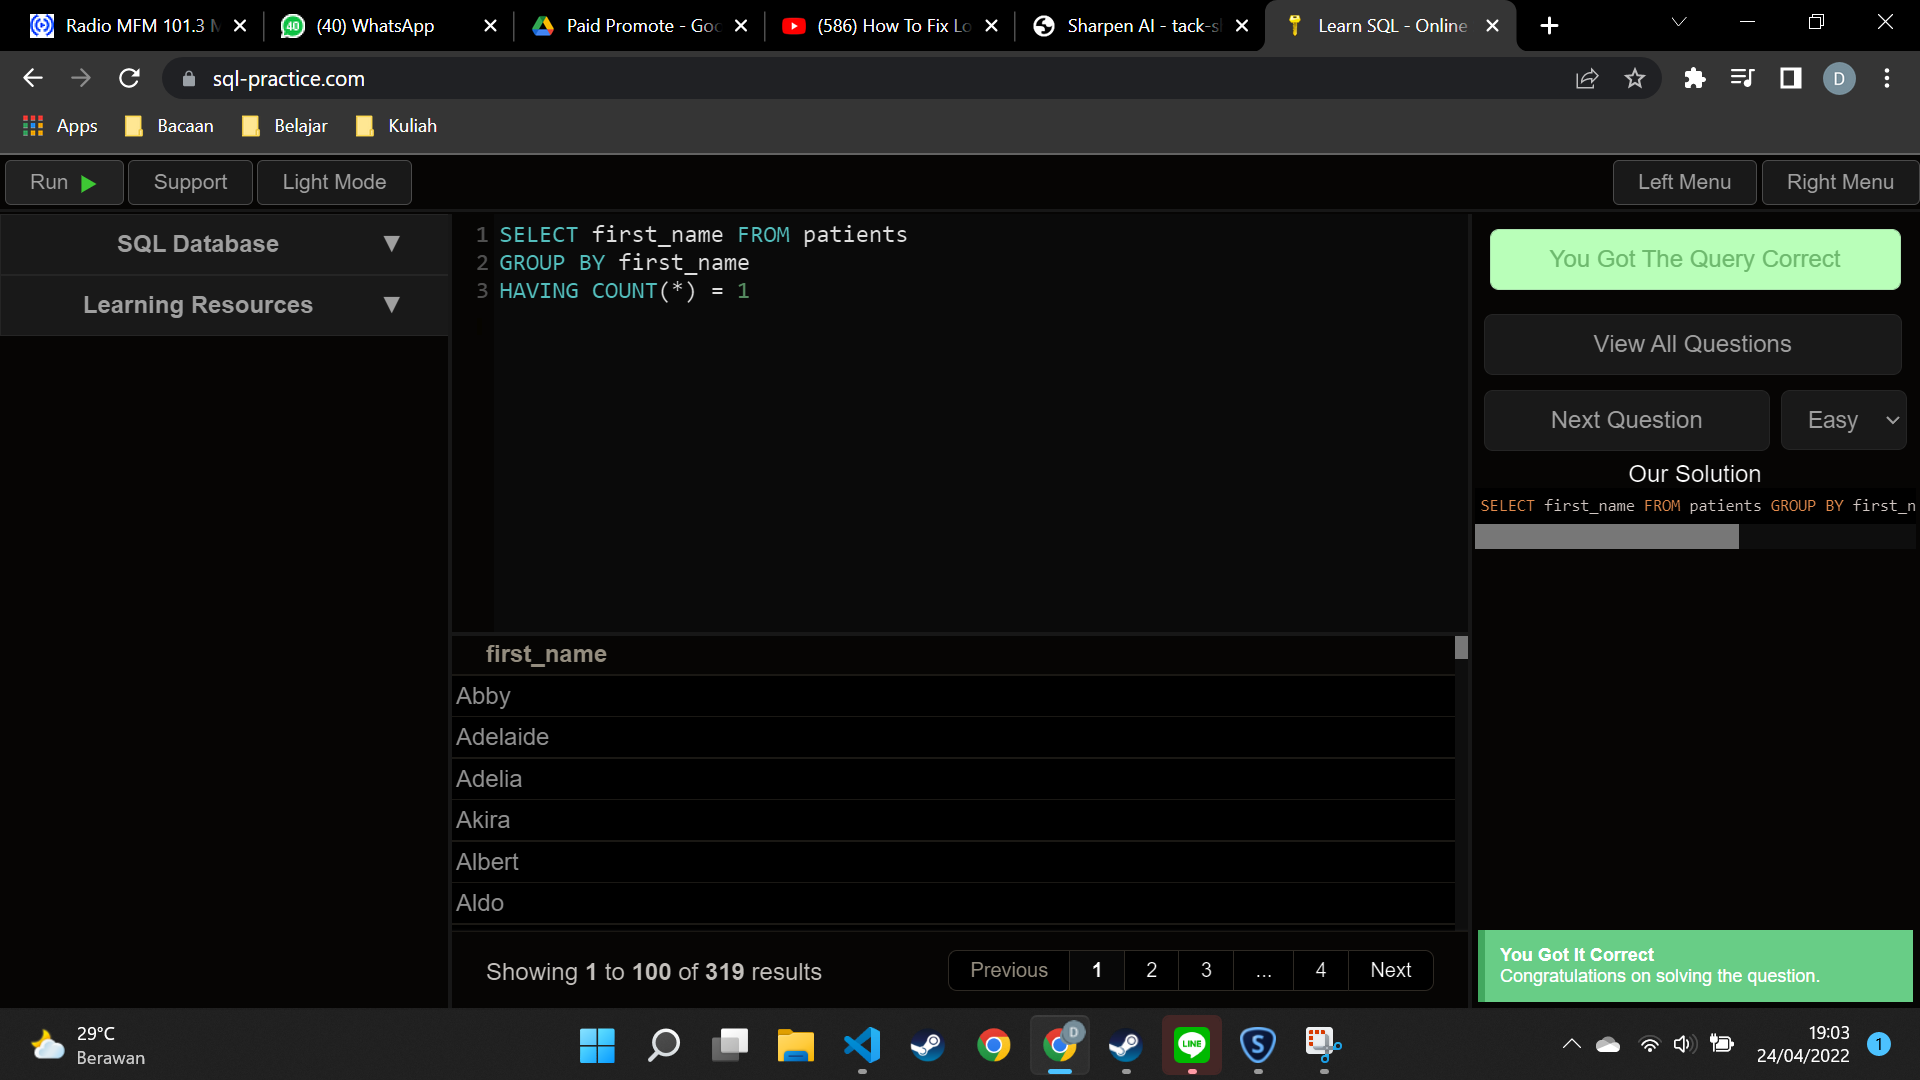
\includegraphics[scale=0.3]{./Screenshot/Medium-2.png}
            \centering
        \end{figure}

        \item Show patient\_id and first\_name from patients where their first\_name start and ends with 's' and is atleast 5 characters long.
        \\Query :
        \lstinputlisting[label={listing14},caption={Medium - 3}, language={sql}]{"../Medium-3.sql"}
        \begin{itemize}
            \item Baris 1 : Mengambil data patient\_id dan first\_name dari tabel patients
            \item Baris 2 : Dengan kondisi dimana first\_name dari pasien diawali dengan huruf "s" yang diikuti minimal 3 karakter dan diakhiri dengan huruf "s" 
        \end{itemize}
        \pagebreak
        Screenshot :
        \begin{figure}[h]
            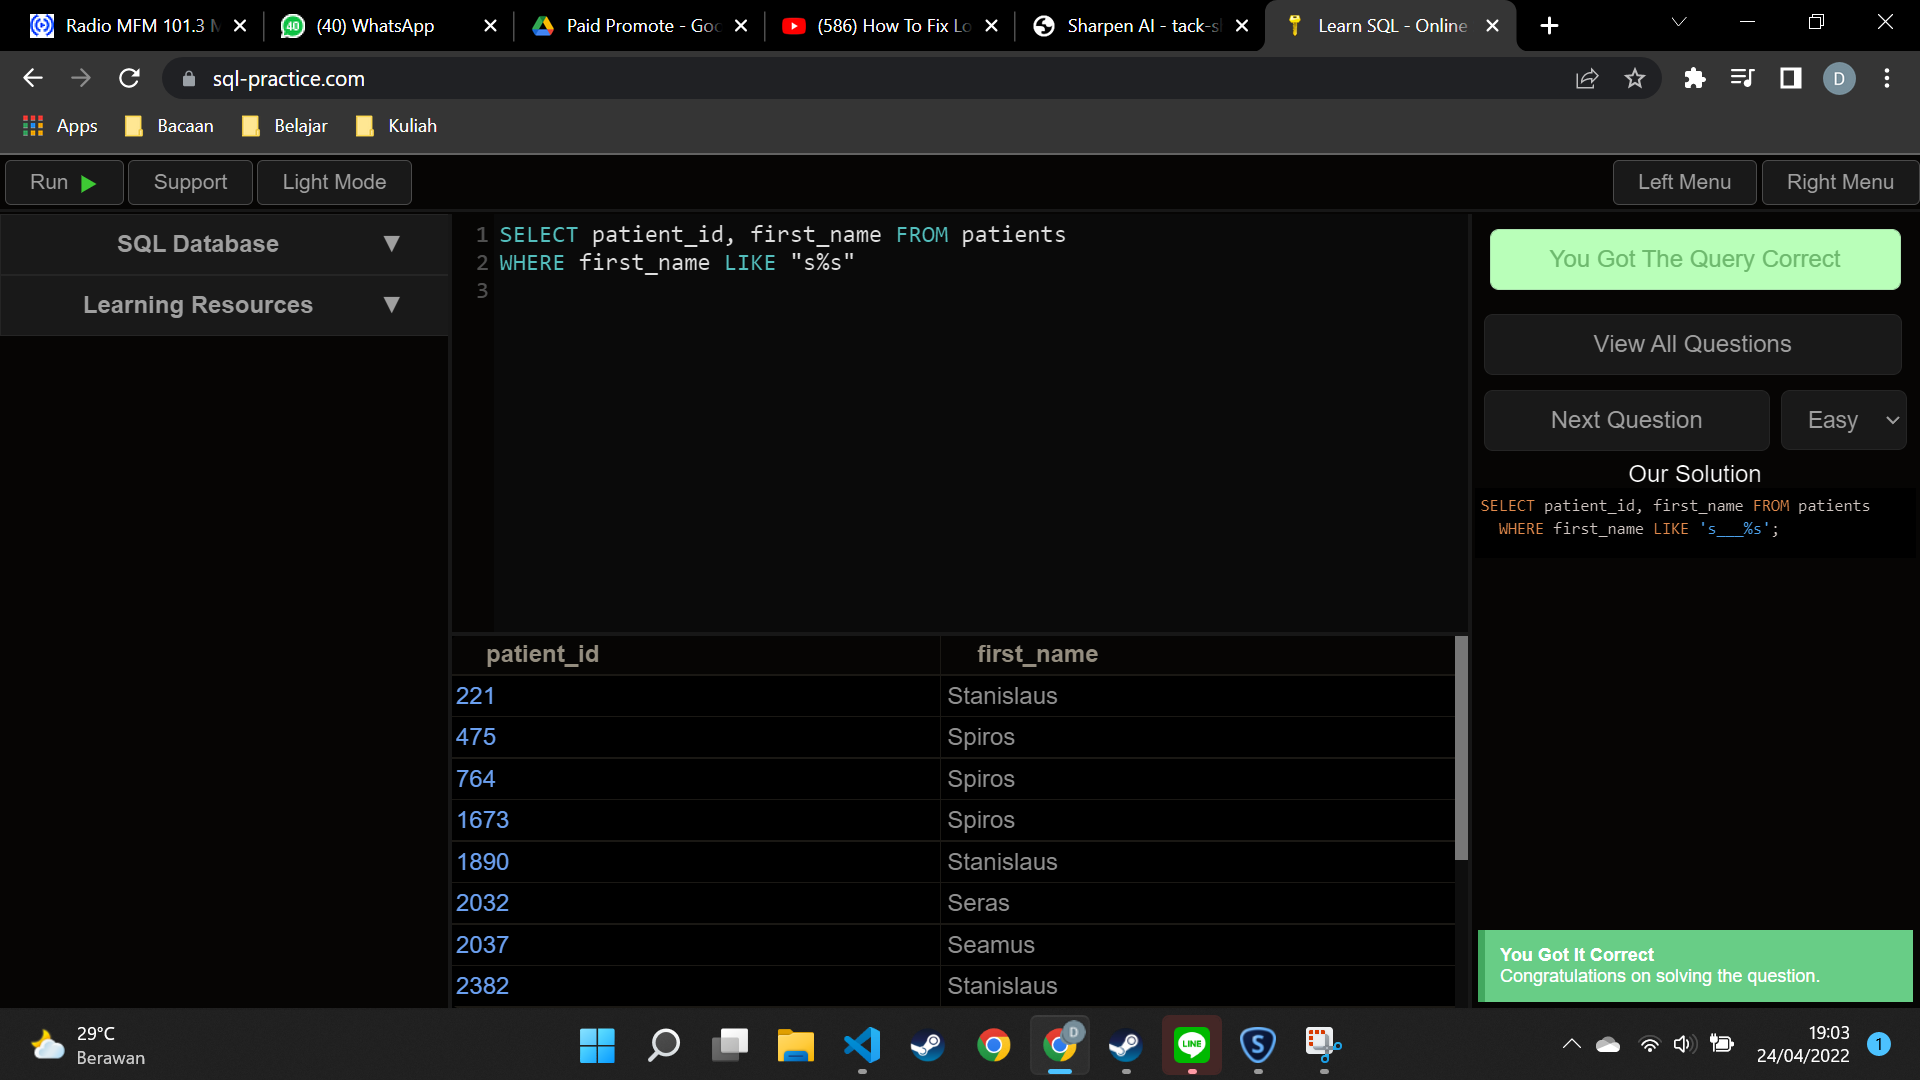
\includegraphics[scale=0.3]{./Screenshot/Medium-3.png}
            \centering
        \end{figure}

        \item Show patient\_id, first\_name, last\_name from patients whos
        \\primary\_diagnosis is 'Dementia'. Primary diagnosis is stored in the admissions table
        \\Query :
        \lstinputlisting[label={listing15},caption={Medium - 4}, language={sql}]{"../Medium-4.sql"}
        \begin{itemize}
            \item Baris 1 : Mengambil data patient\_id, first\_name dan last\_name dari tabel patients
            \item Baris 2 : Menggabungkan tabel admissions sesuai data dari tabel patients
            \item Baris 3 : Dengan acuan patient\_id pada tabel patients merujuk pada patient\_id pada tabel admissions
            \item Baris 4 : Mengambil data dengan kondisi dimana primary\_diagnosis dari pasien adalah "Dementia"
        \end{itemize}
        \pagebreak
        Screenshot :
        \begin{figure}[h]
            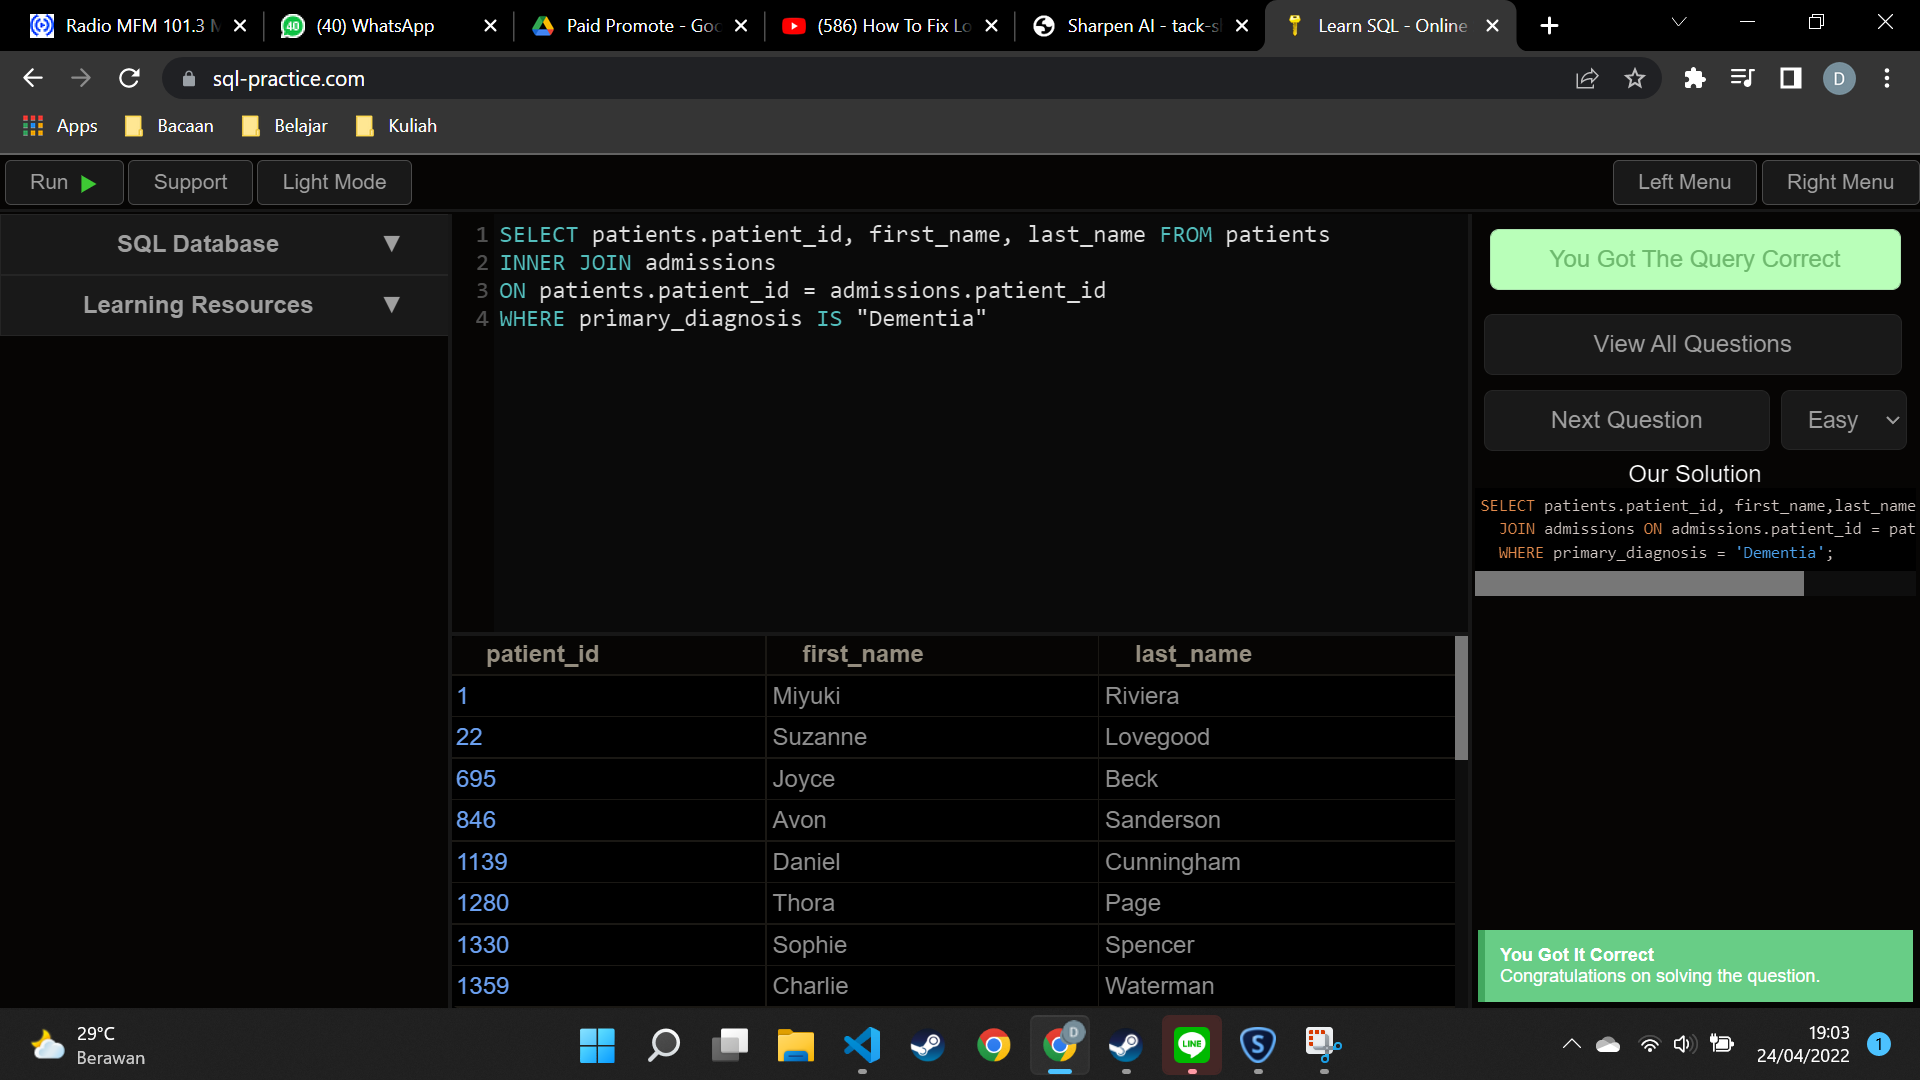
\includegraphics[scale=0.3]{./Screenshot/Medium-4.png}
            \centering
        \end{figure}

        \item Show patient\_id, first\_name, last\_name from the patients table.
        Order the rows by the first\_name ascending and then by the last\_name descending
        \\Query :
        \lstinputlisting[label={listing16},caption={Medium - 5}, language={sql}]{"../Medium-5.sql"}
        \begin{itemize}
            \item Baris 1 : Mengambil data patient\_id, first\_name, dan last\_name dari tabel patients
            \item Baris 2 : Mengurutkan berdasarkan first\_name secara ascending lalu mengurutkan berdasarkan last\_name secara descending
        \end{itemize}
        Screenshot :
        \begin{figure}[h]
            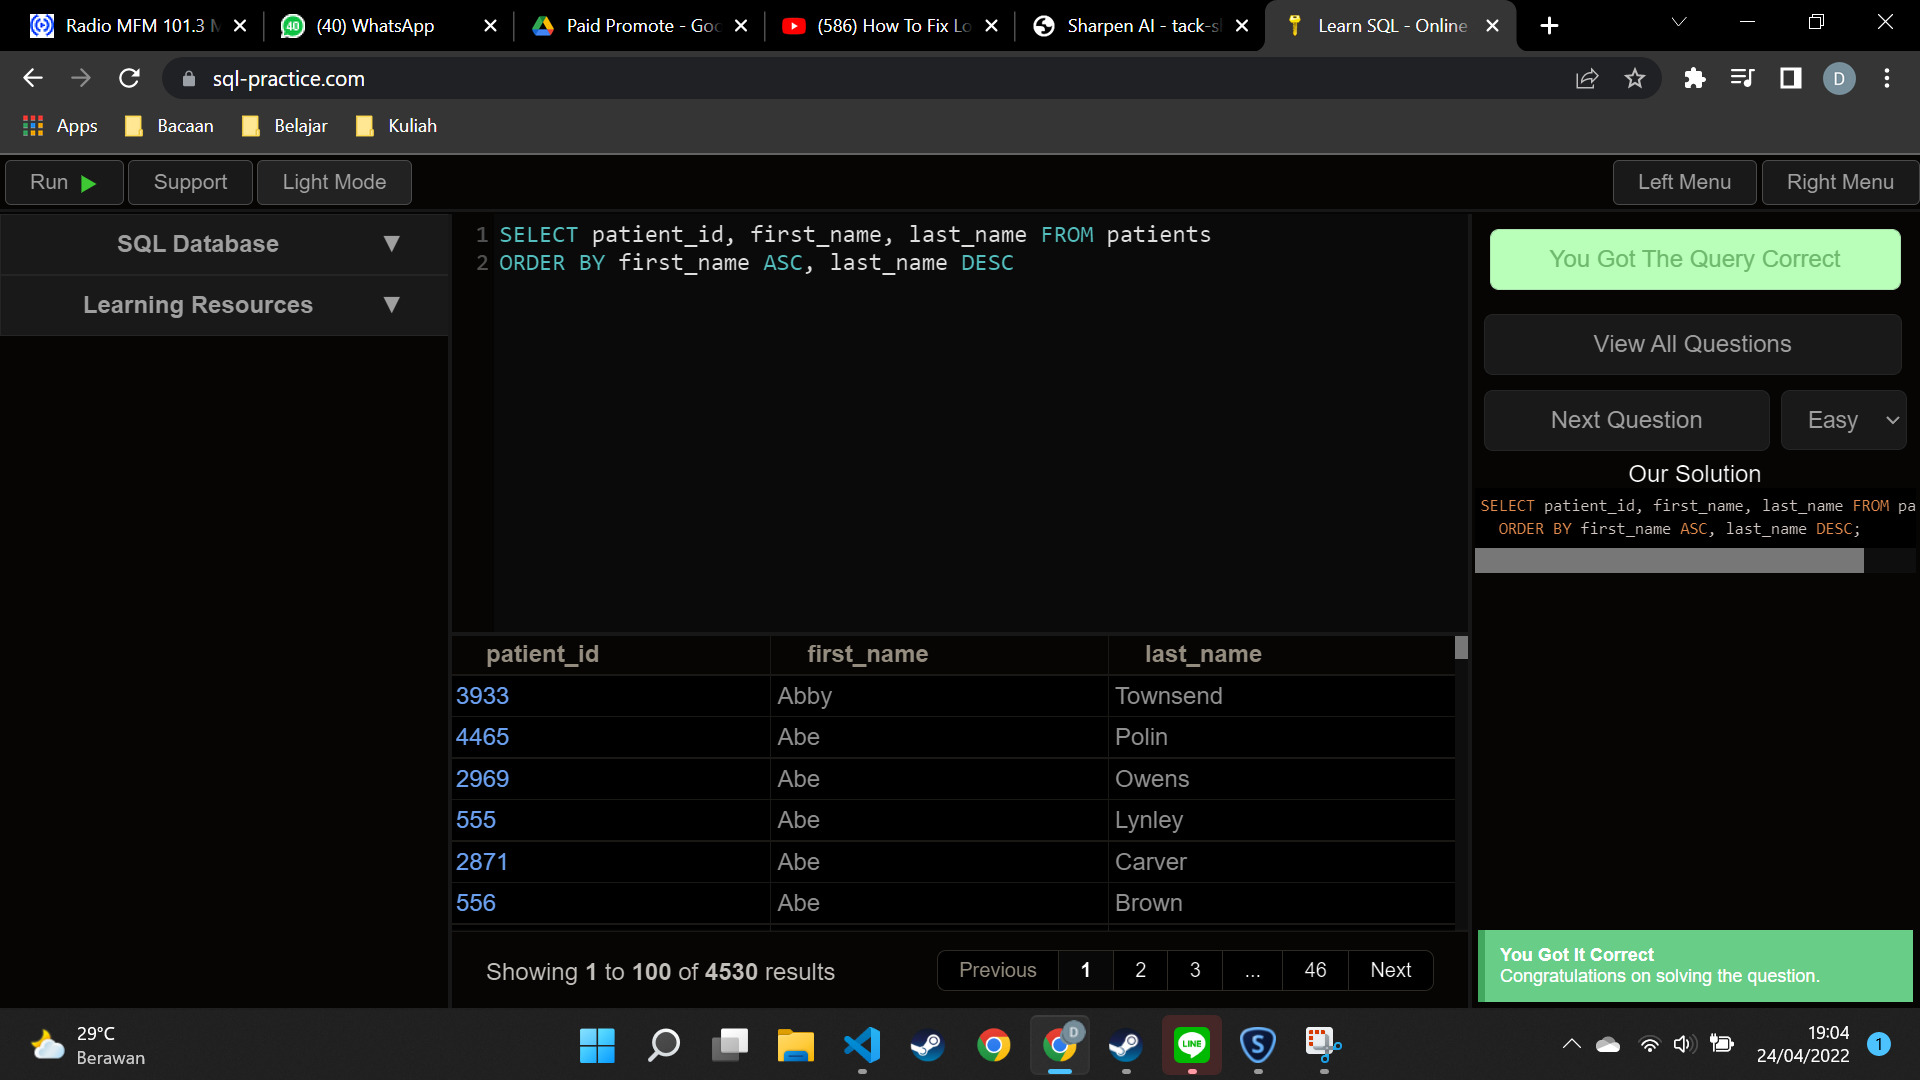
\includegraphics[scale=0.3]{./Screenshot/Medium-5.png}
            \centering
        \end{figure}

        \item Show the total amount of male patients and the total amount of female patients in the patients table
        \\Query :
        \lstinputlisting[label={listing17},caption={Medium - 6}, language={sql}]{"../Medium-6.sql"}
        \begin{itemize}
            \item Baris 1 : Mengambil banyaknya data yang memiliki gender "M" (selanjutnya akan disebut male\_count) dan banyaknya data yang memiliki gender "F" (selanjutnya akan disebut female\_count) dari tabel patients 
        \end{itemize}
        Screenshot :
        \begin{figure}[h]
            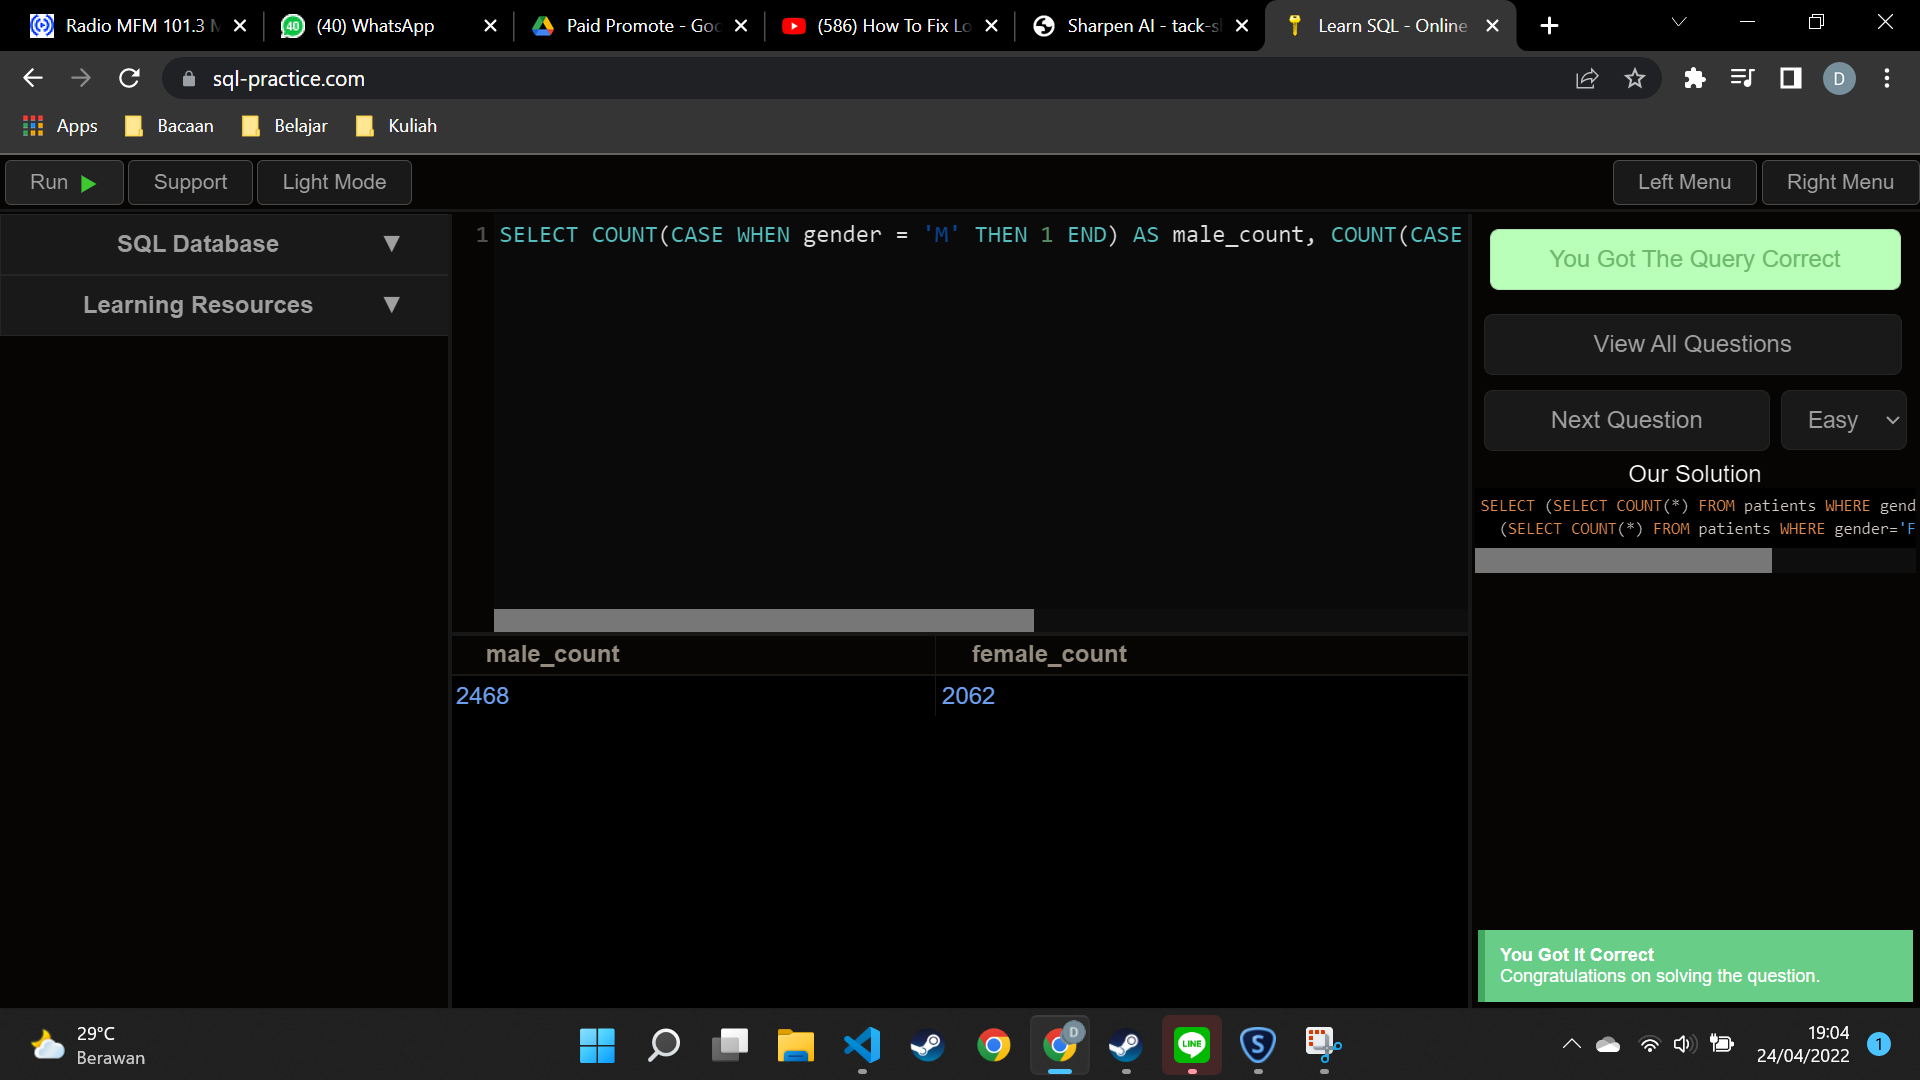
\includegraphics[scale=0.3]{./Screenshot/Medium-6.png}
            \centering
        \end{figure}

        \item Show first and last name, allergies from patients which have allergies to either 'Penicillin' or 'Morphine'. Show results ordered ascending by allergies then by first\_name then by last\_name.
        \\Query :
        \lstinputlisting[label={listing18},caption={Medium - 7}, language={sql}]{"../Medium-7.sql"}
        \begin{itemize}
            \item Baris 1 : Mengambil data first\_name, last\_name, dan allergies dari tabel patients
            \item Baris 2 : Dengan kondisi dimana allergies yang dimiliki pasien adalah "Penicillin" atau "Morphine"
            \item Baris 3 : Mengurutkan data berdasarkan allergies secara ascending, lalu mengurutkan data berdasarkan first\_name secara ascending, dan terakhir mengurutkan data berdasarkan last\_name secara ascending
        \end{itemize}
        Screenshot :
        \begin{figure}[h]
            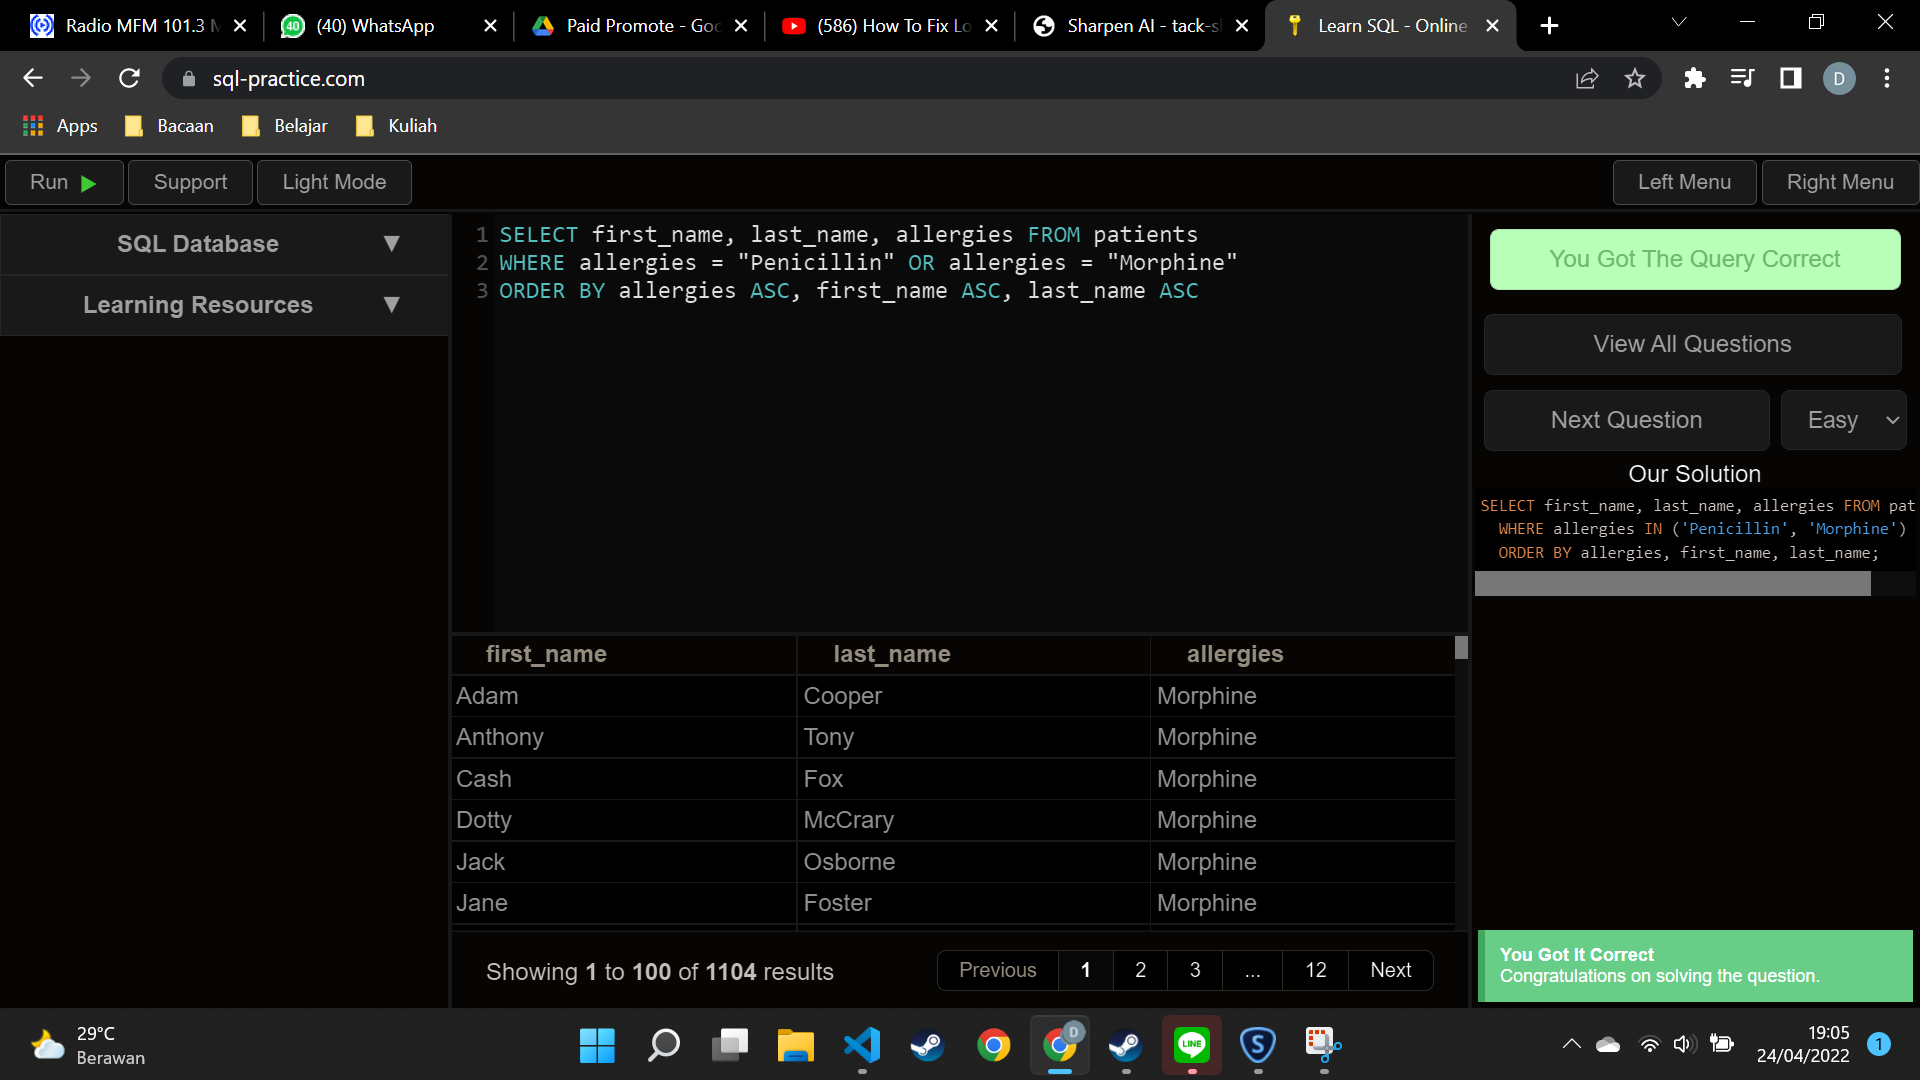
\includegraphics[scale=0.3]{./Screenshot/Medium-7.png}
            \centering
        \end{figure}

        \item Show patient\_id, primary\_diagnosis from admissions. Find patients admitted multiple times for the same primary\_diagnosis
        \\Query :
        \lstinputlisting[label={listing19},caption={Medium - 8}, language={sql}]{"../Medium-8.sql"}
        \begin{itemize}
            \item Baris 1 : Mengambil data patient\_id dan primary\_diagnosis dari tabel admissions
            \item Baris 2 : Mengelompokkan berdasarkan patient\_id, lalu Mengelompokkan berdasarkan primary\_diagnosis
            \item Baris 3 : Mengambil data dalam kelompok yang memiliki anggota lebih dari 1 (pasien yang sama terkena penyakit yang sama lebih dari sekali)
        \end{itemize}
        \pagebreak
        Screenshot :
        \begin{figure}[h]
            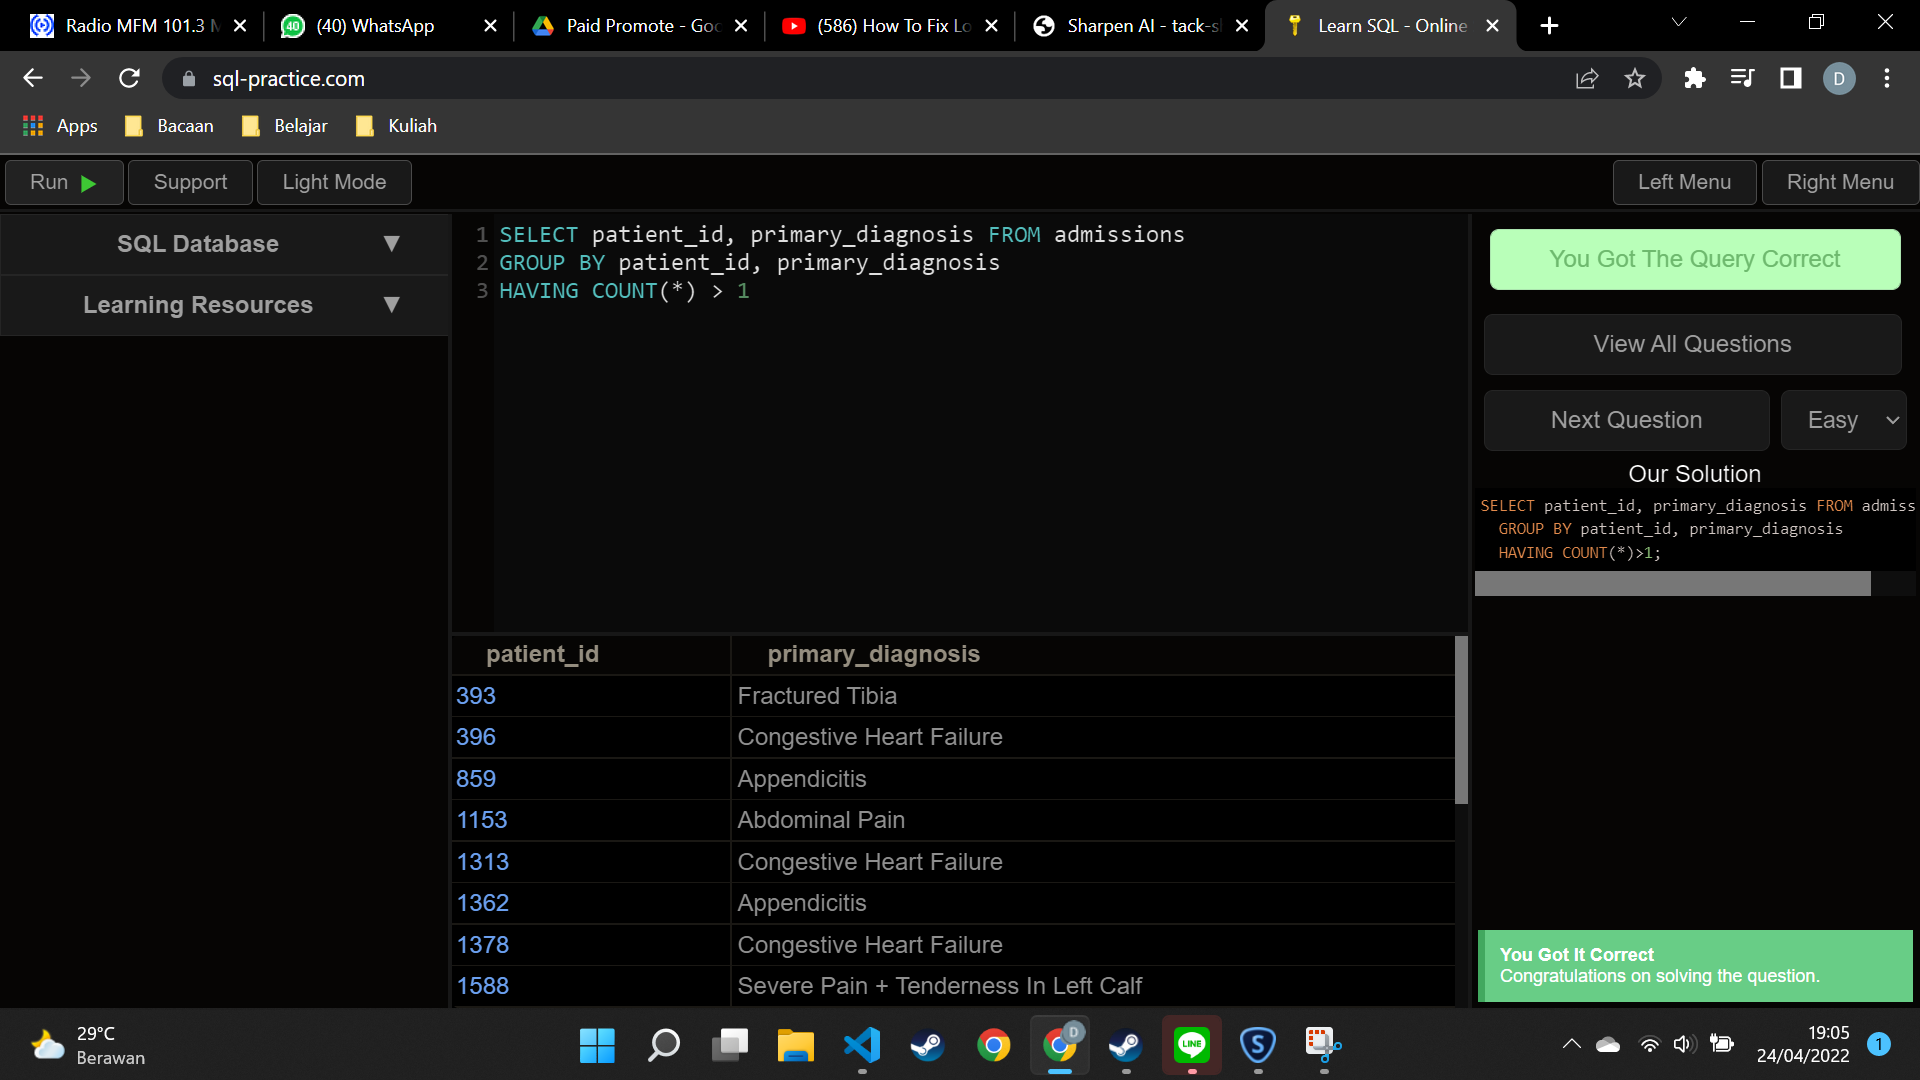
\includegraphics[scale=0.3]{./Screenshot/Medium-8.png}
            \centering
        \end{figure}

        \item Show the city and the total number of patients in the city in the order from most to least patients
        \\Query :
        \lstinputlisting[label={listing20},caption={Medium - 9}, language={sql}]{"../Medium-9.sql"}
        \begin{itemize}
            \item Baris 1 : Mengambil data city dan banyaknya data (akan disebut sebagai num\_patients) dari tabel patients
            \item Baris 2 : Mengelompokkan data berdasarkan city
            \item Baris 3 : Mengurutkan data berdasarkan num\_patients secara descending
        \end{itemize}
        \pagebreak
        Screenshot :
        \begin{figure}[h]
            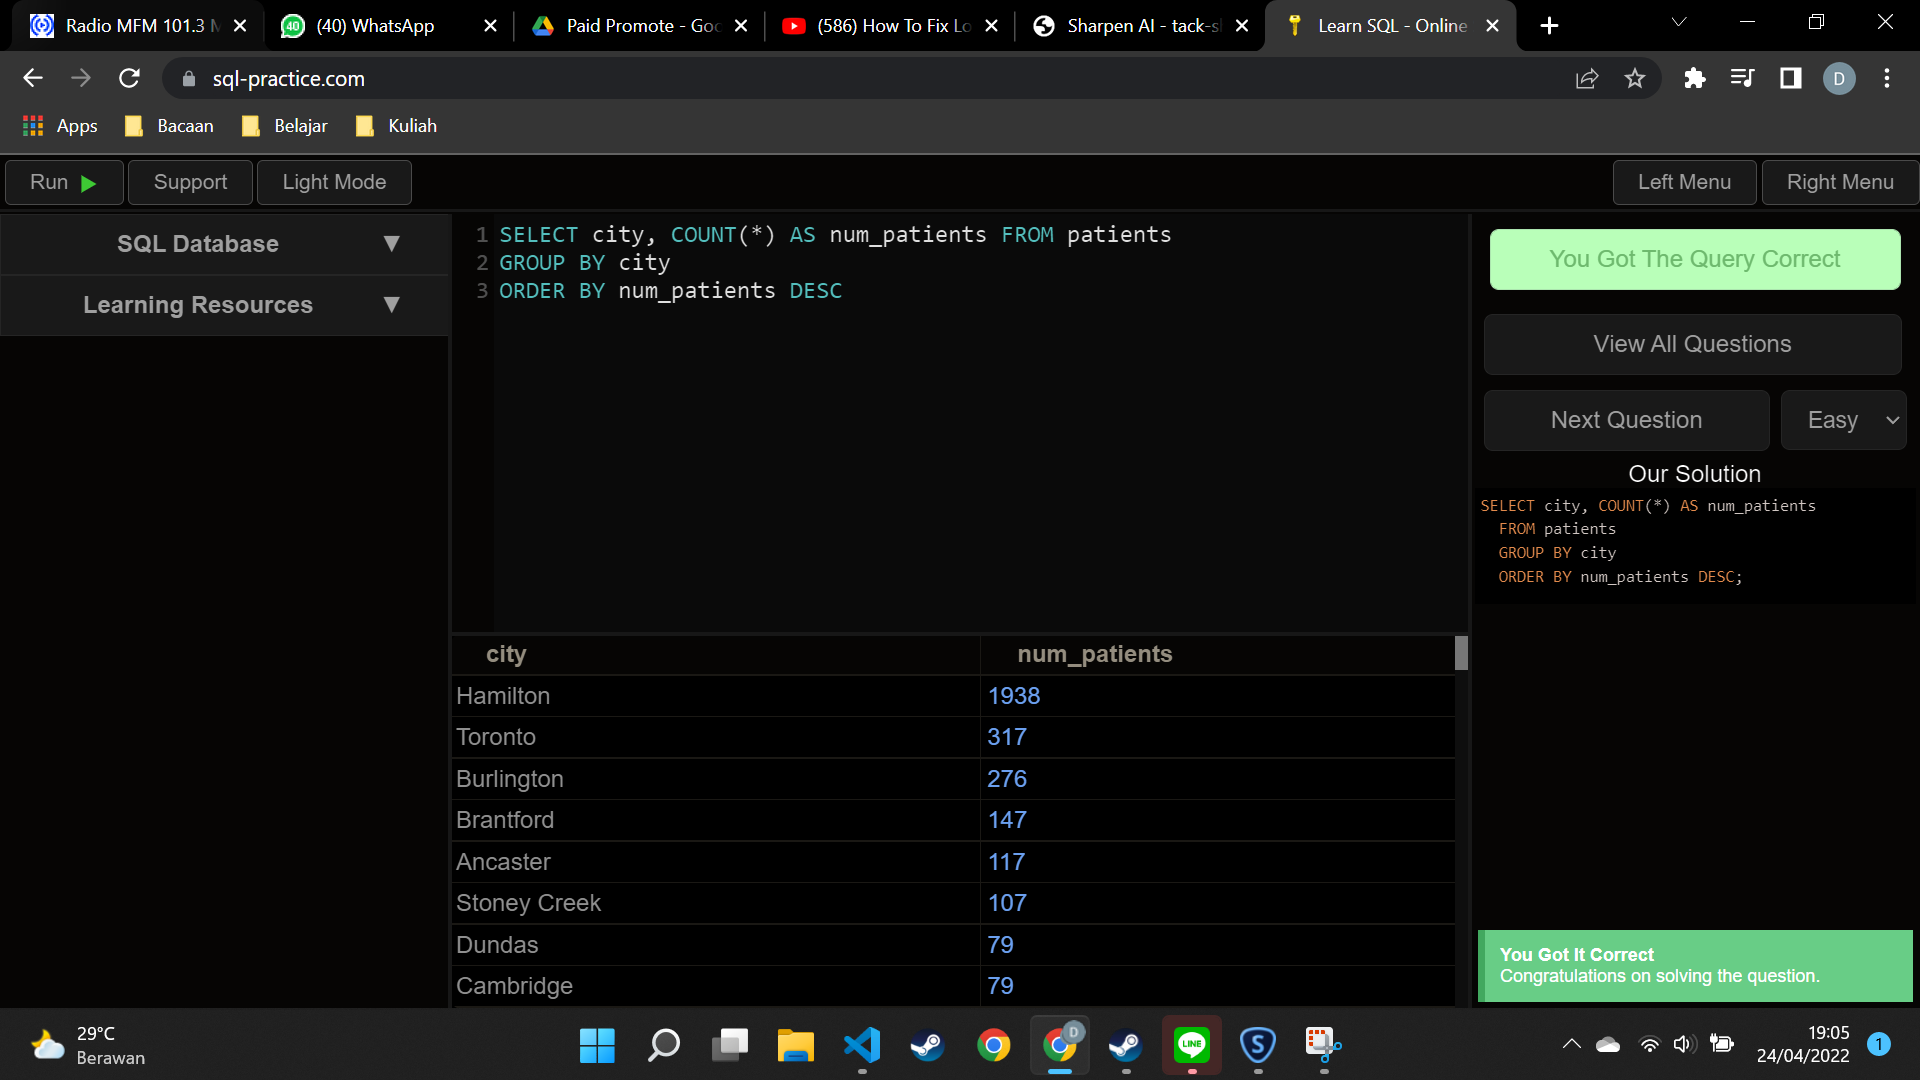
\includegraphics[scale=0.3]{./Screenshot/Medium-9.png}
            \centering
        \end{figure}

        \item Show first name, last name and role of every person that is either patient or physician. The roles are either "Patient" or "Physician"
        \\Query :
        \lstinputlisting[label={listing21},caption={Medium - 10}, language={sql}]{"../Medium-10.sql"}
        \begin{itemize}
            \item Baris 1 : Mengambil tabel patients
            \item Baris 2 : Menambahkan kolom Role sebagai tipe data varchar
            \item Baris 3 : Mengambil tabel physicians
            \item Baris 4 : Menambahkan kolom Role sebagai tipe data varchar
            \item Baris 5 : Mengupdate tabel patients
            \item Baris 6 : Mengubah nilai Role pada tabel patients dengan "Patient"
            \item Baris 7 : Mengupdate tabel patients
            \item Baris 8 : Mengubah nilai Role pada tabel physicians dengan "Physician"
            \item Baris 9 - 10 : Menambahkan nilai dari tabel physicians ke tabel patients
            \item Baris 11 : Mengambil data first\_name, last\_name, dan Role dari tabel patients
            \item Baris 12 : Mengurutkan berdasarkan first\_name secara ascending, lalu mengurutkan berdasarkan last\_name secara ascending
        \end{itemize}
        Screenshot :
        \begin{figure}[h]
            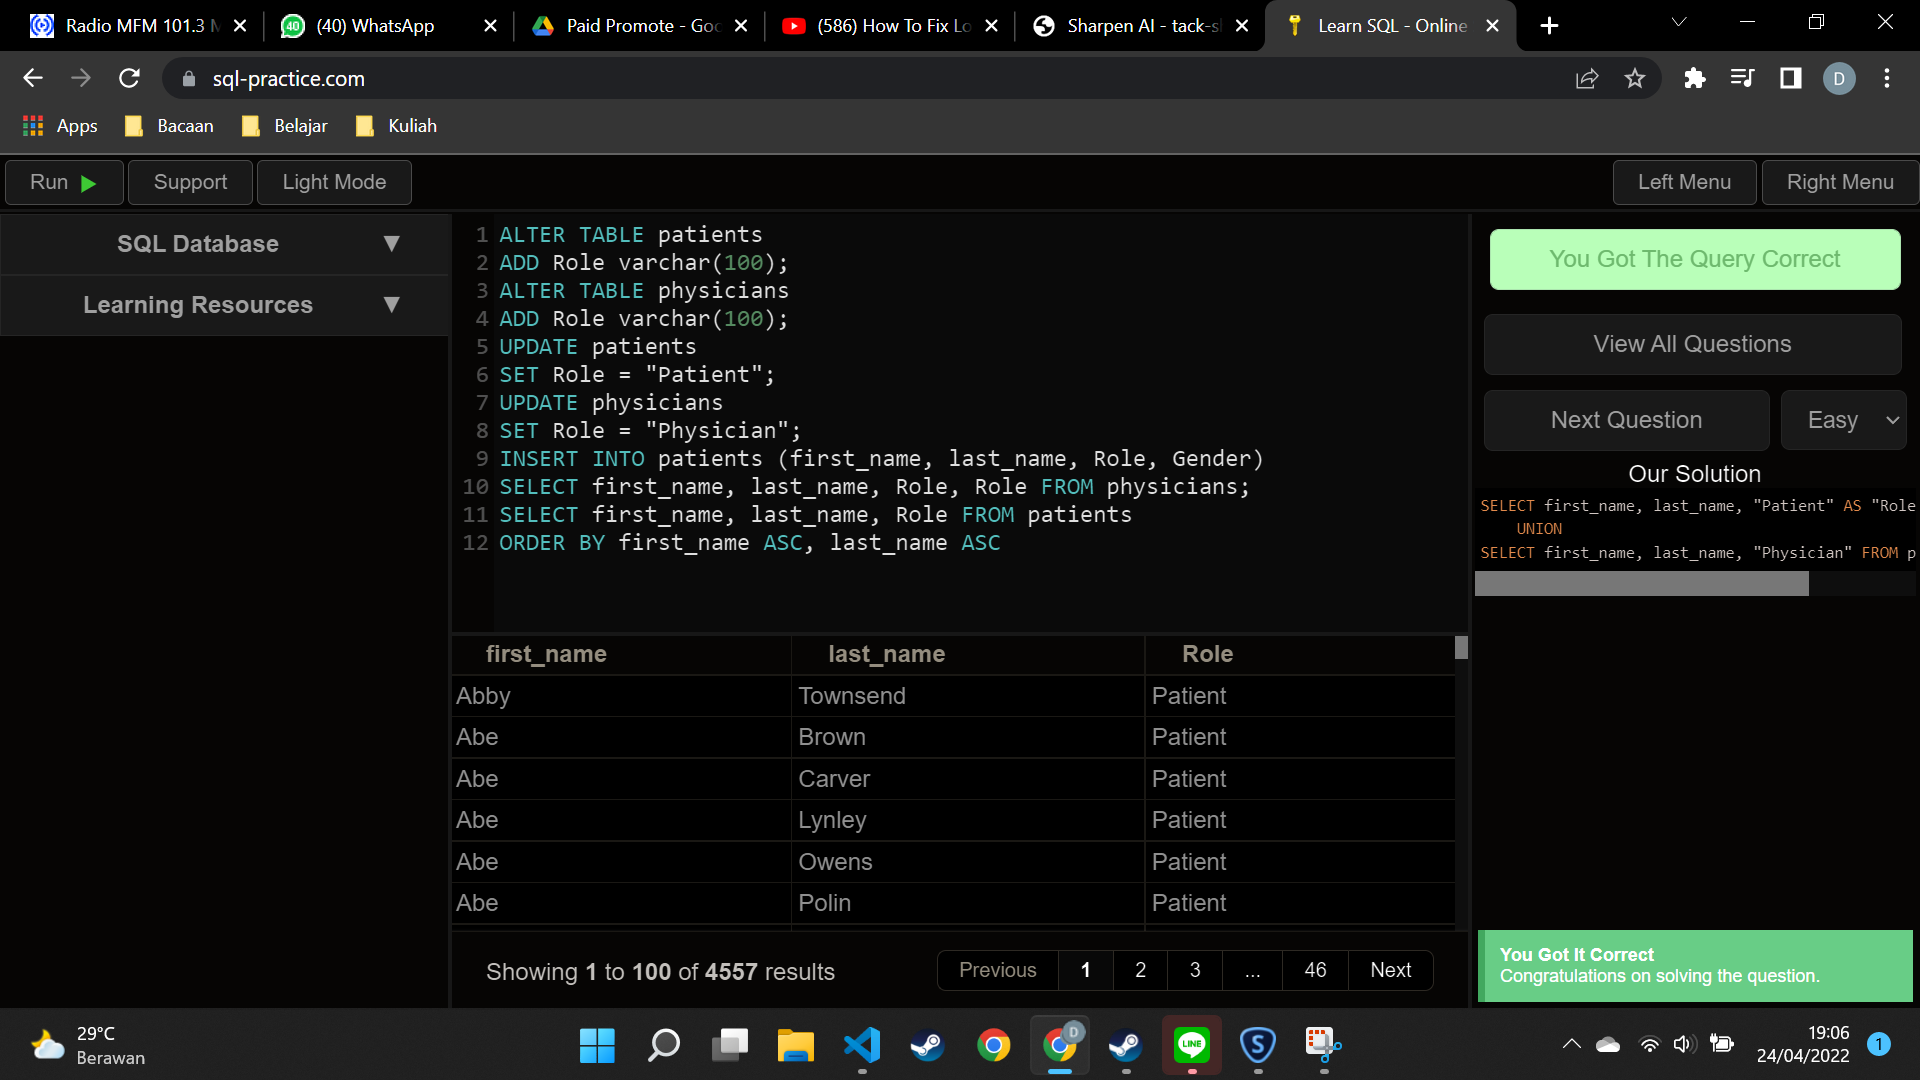
\includegraphics[scale=0.3]{./Screenshot/Medium-10.png}
            \centering
        \end{figure}

        \item Show all allergies ordered by popularity. Remove 'NKA' and NULL values from query
        \\Query :
        \lstinputlisting[label={listing22},caption={Medium - 11}, language={sql}]{"../Medium-11.sql"}
        \begin{itemize}
            \item Baris 1 : Mengambil data allergies dan banyaknya data sebagai total\_diagnose dari tabel patients
            \item Baris 2 : Dengan kondisi dimana allergies yang dimiliki adalah selain NKA dan tidak bernilai null
            \item Baris 3 : Mengelompokkan data berdasarkan allergies
            \item Baris 4 : Mengurutkan data berdasarkan banyaknya data dari tiap kelompok secara descending
        \end{itemize}
        \pagebreak
        Screenshot :
        \begin{figure}[h]
            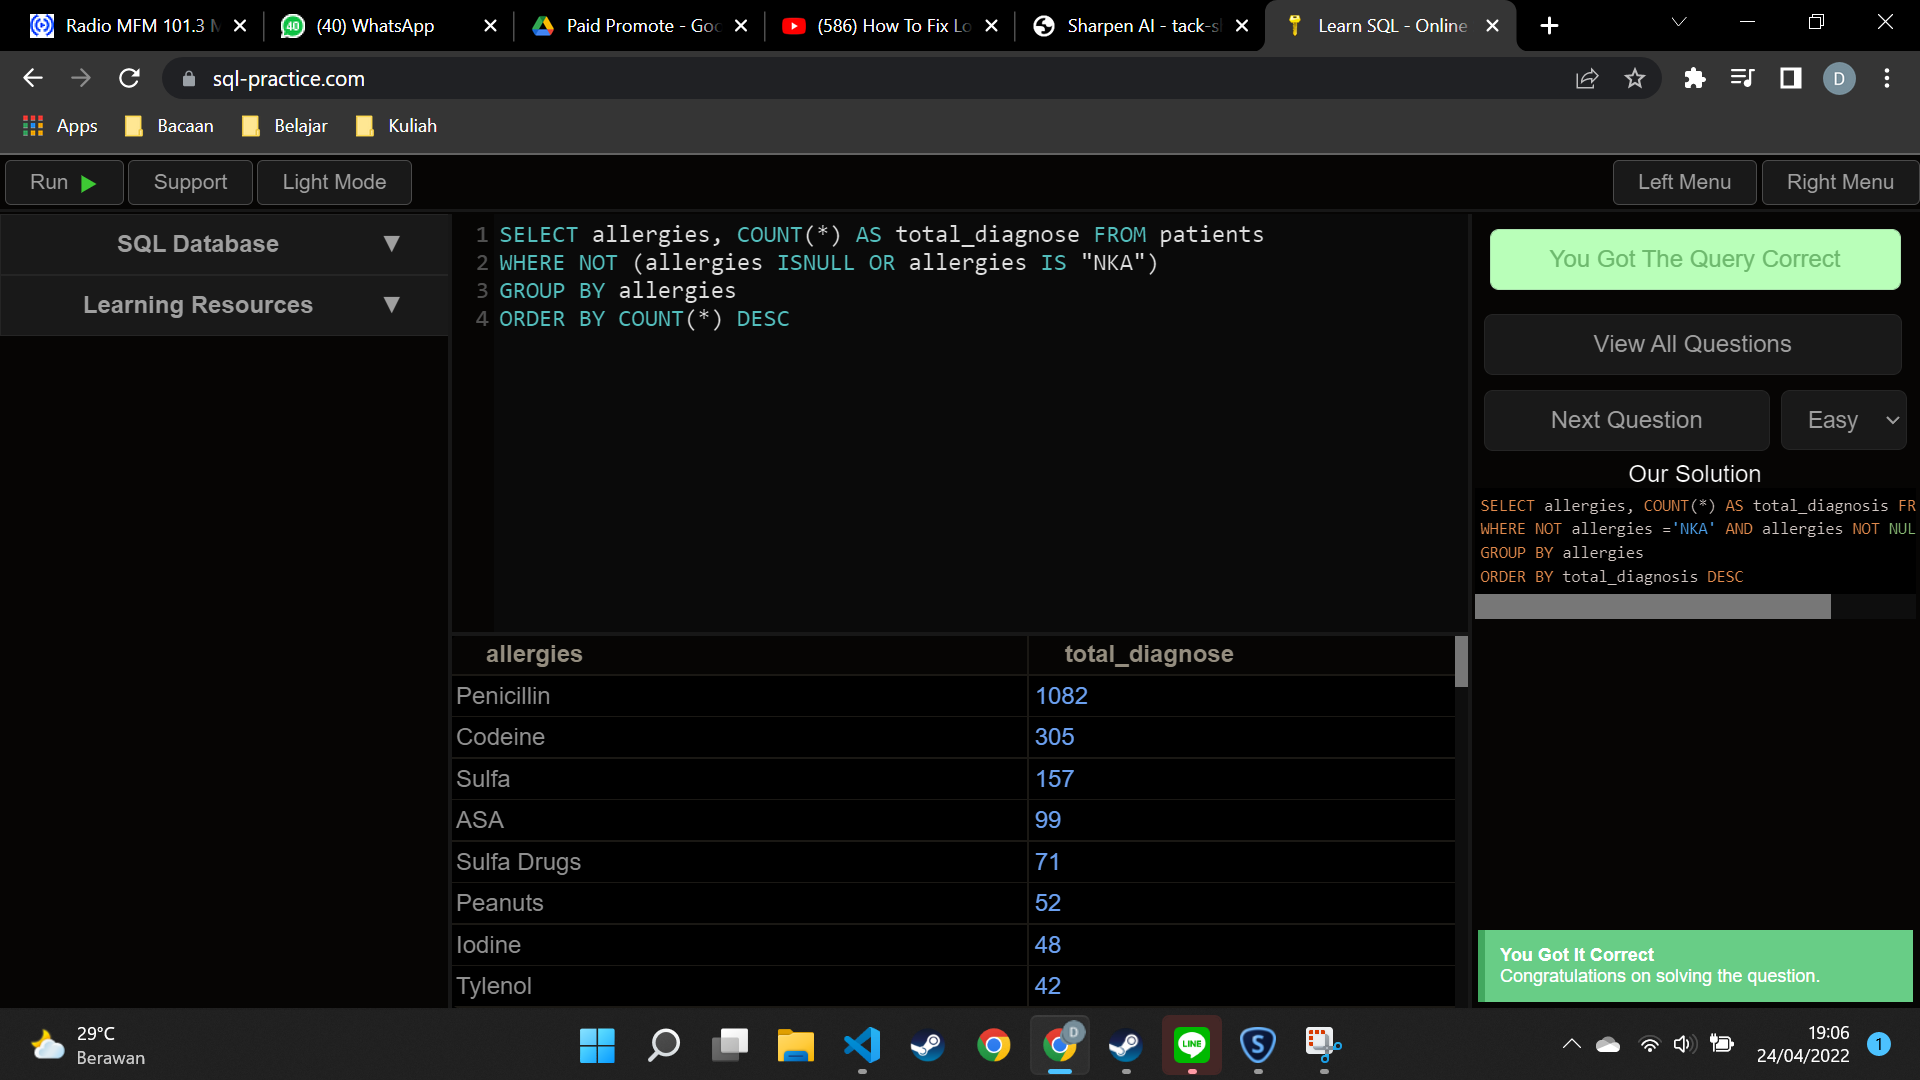
\includegraphics[scale=0.3]{./Screenshot/Medium-11.png}
            \centering
        \end{figure}

        \item Show all patient's first\_name, last\_name, and birth\_date who were born in the 1970s decade. Sort the list starting from the earliest birth\_date.
        \\Query :
        \lstinputlisting[label={listing23},caption={Medium - 12}, language={sql}]{"../Medium-12.sql"}
        \begin{itemize}
            \item Baris 1 : Mengambil data first\_name, last\_name, dan height dari tabel patients
            \item Baris 2 : Dengan kondisi dimana modulus dari tahun lahir dengan 1970 adalah kurang dari 10 (1970 - 1979)
            \item Baris 3 : Mengurutkan data berdasarkan birth\_date secara ascending
        \end{itemize}
        \pagebreak
        Screenshot :
        \begin{figure}[h]
            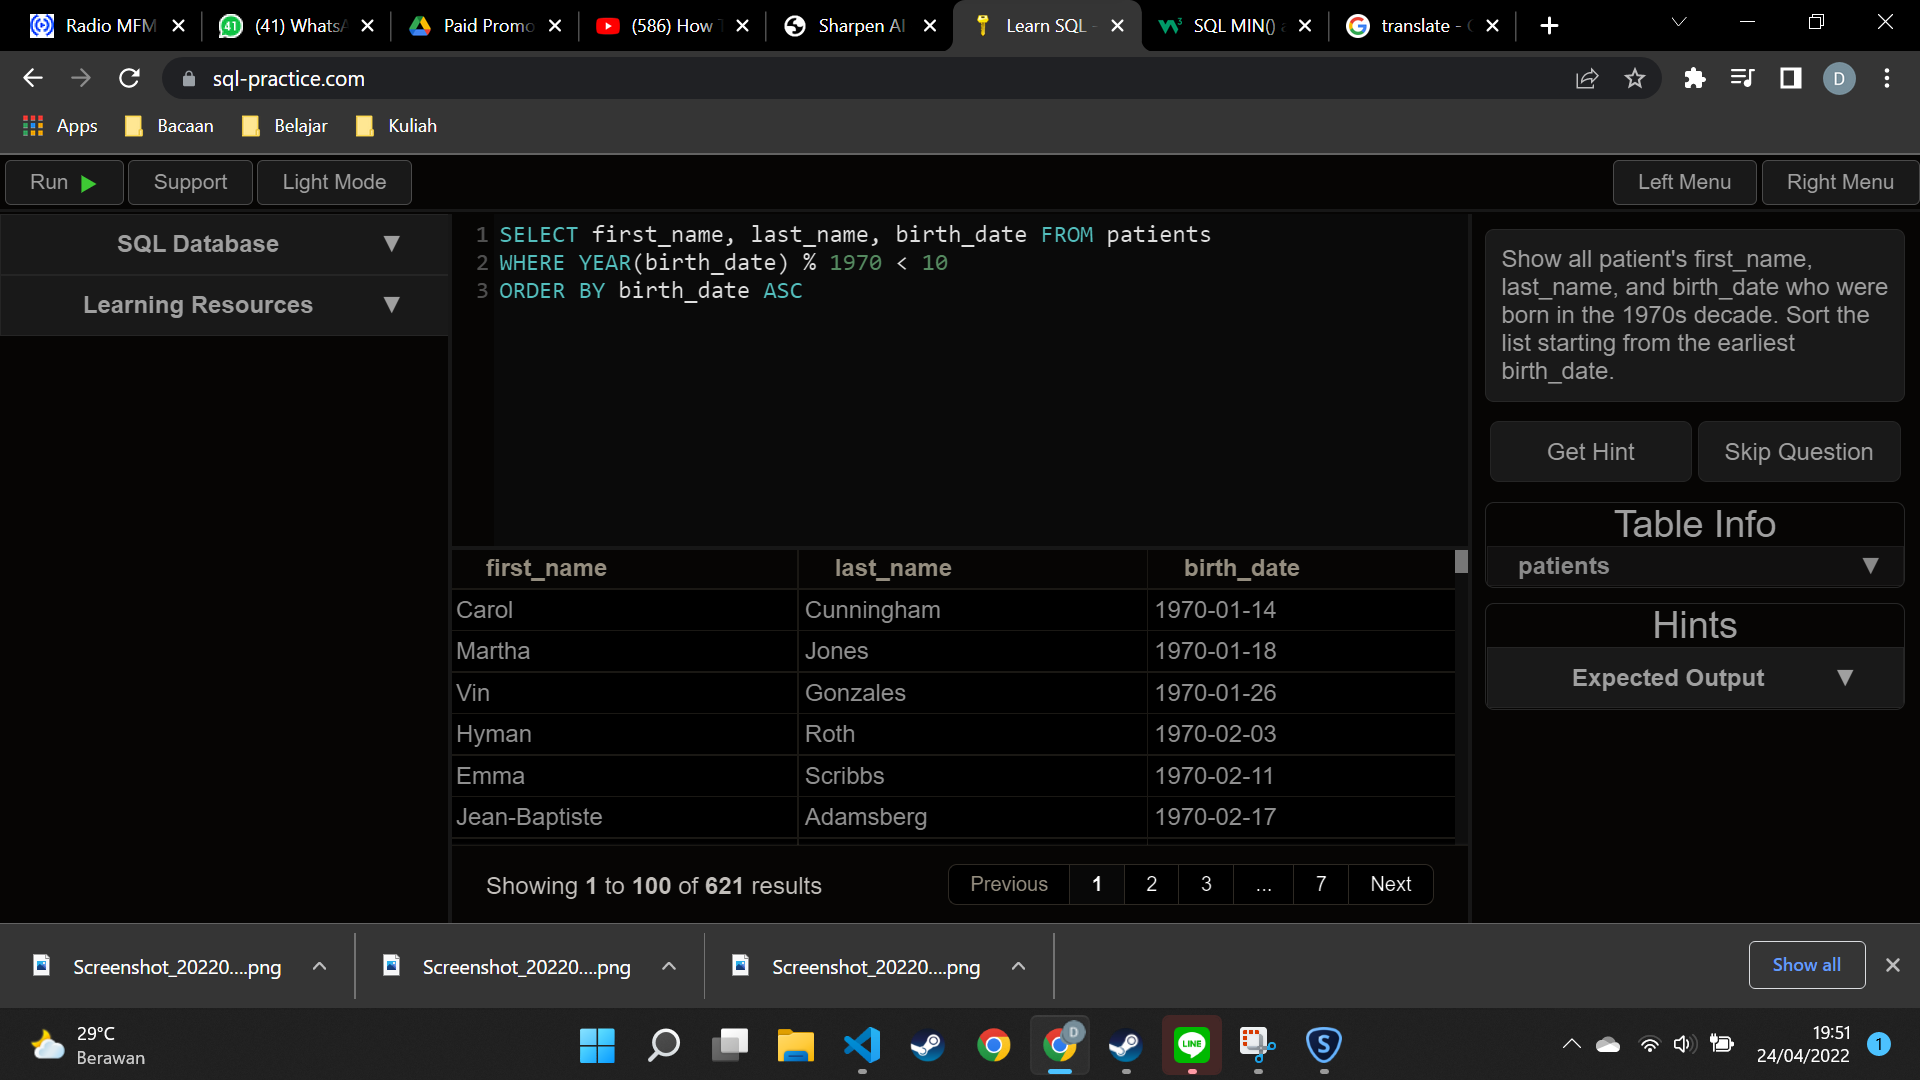
\includegraphics[scale=0.3]{./Screenshot/Medium-12.png}
            \centering
        \end{figure}

        \item We want to display each patient's full name in a single column. Their last\_name in all upper letters must appear first, then first\_name in all lower case letters. Separate the last\_name and first\_name with a comma. Order the list by the first\_name in decending order. EX: SMITH,jane
        \\Query :
        \lstinputlisting[label={listing24},caption={Medium - 13}, language={sql}]{"../Medium-13.sql"}
        \begin{itemize}
            \item Baris 1 : Mengambil data gabungan dari last\_name yang diubah uppercase, tanda ",", dan first\_name yang diubah lowercase (akan disebut sebagai new\_name\_format) dari tabel patients
            \item Baris 2 : Mengurutkan data berdasarkan first\_name secara descending
        \end{itemize}
        \pagebreak
        Screenshot :
        \begin{figure}[h]
            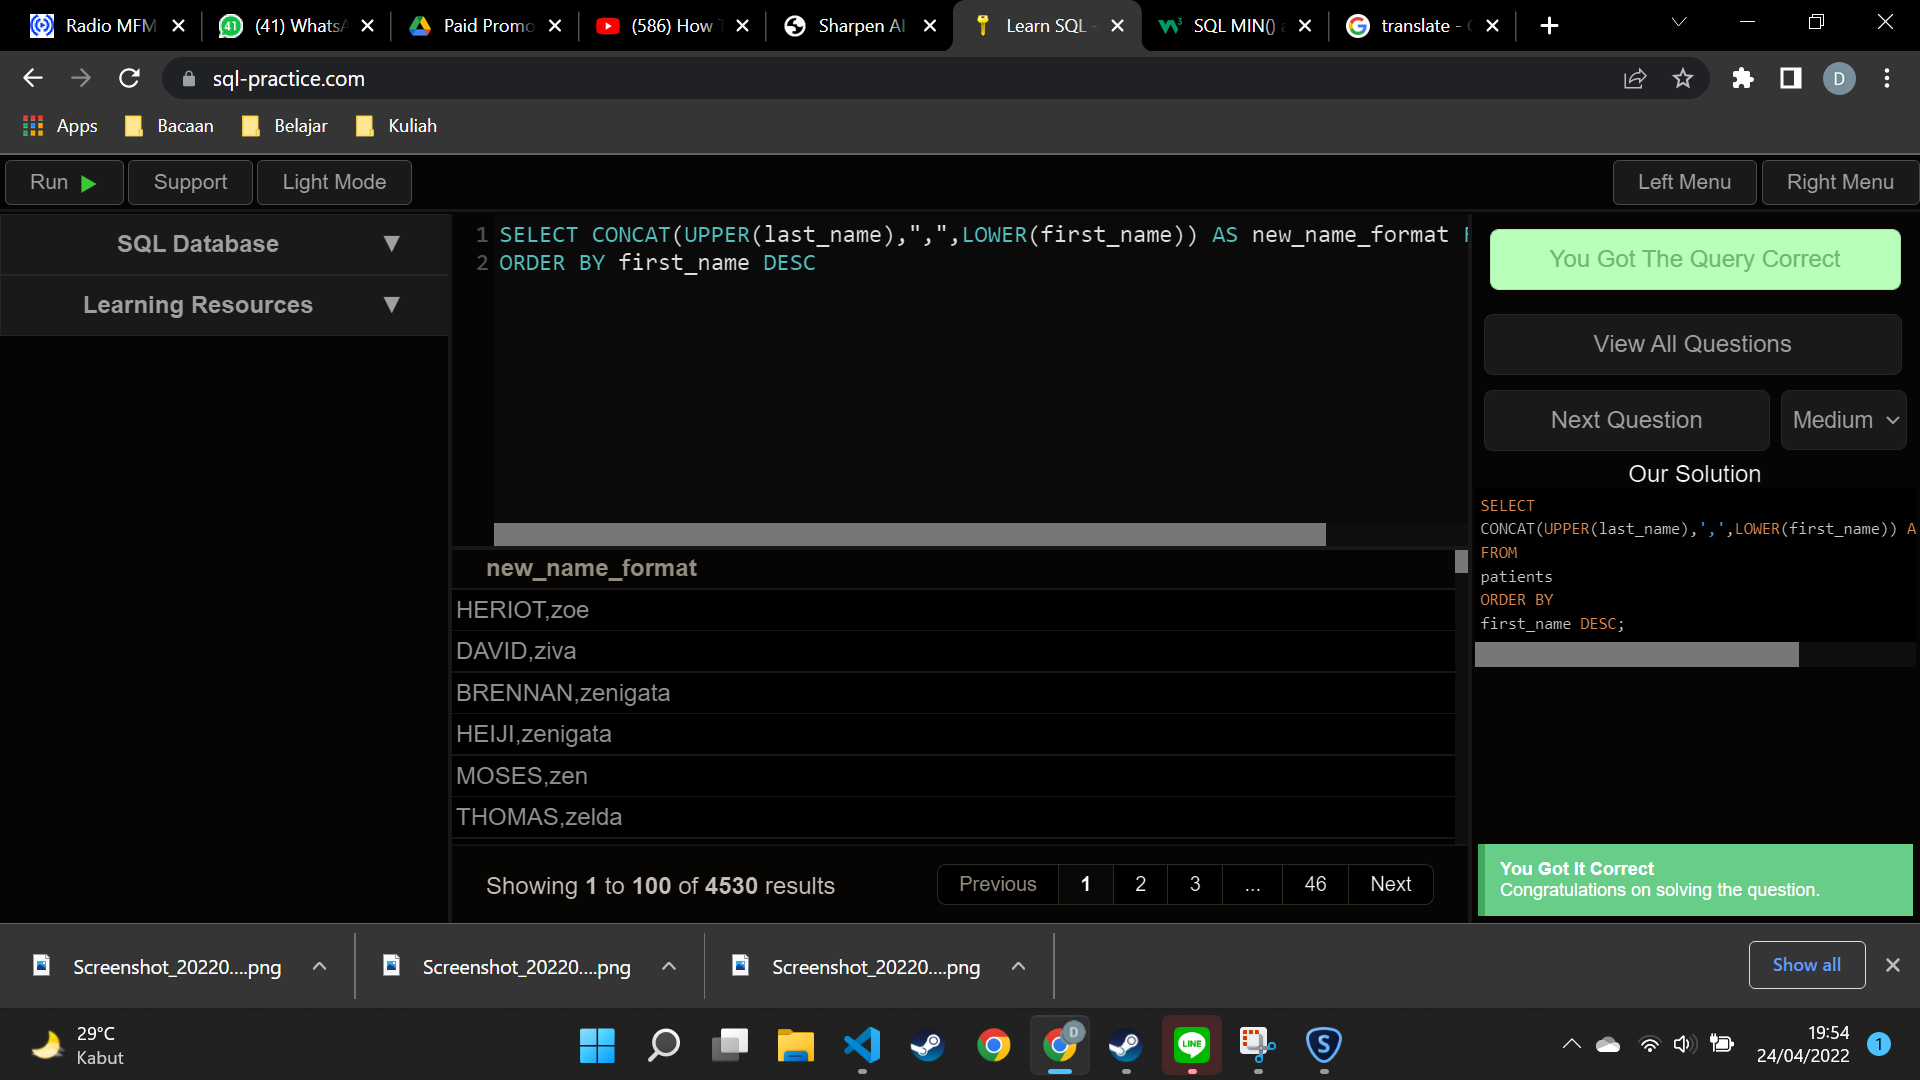
\includegraphics[scale=0.3]{./Screenshot/Medium-13.png}
            \centering
        \end{figure}

        \item Show the cities where the patient's average weight, rounded-up, is less than 70kg. Sort the list by highest to lowest avg\_weight.
        \\Query :
        \lstinputlisting[label={listing25},caption={Medium - 14}, language={sql}]{"../Medium-14.sql"}
        \begin{itemize}
            \item Baris 1 : Mengambil data city, pembulatan keatas dari rata-rata weight (akan disebut sebagai avg\_weight) dari tabel patients
            \item Baris 2 : Mengelompokkan data berdasarkan city
            \item Baris 3 : Dengan kondisi dimana hasil pembulatan keatas dari rata-rata weight kurang dari 70 kg
            \item Baris 4 : Mengurutkan data berdasarkan avg\_weight secara descending
        \end{itemize}
        \pagebreak
        Screenshot :
        \begin{figure}[h]
            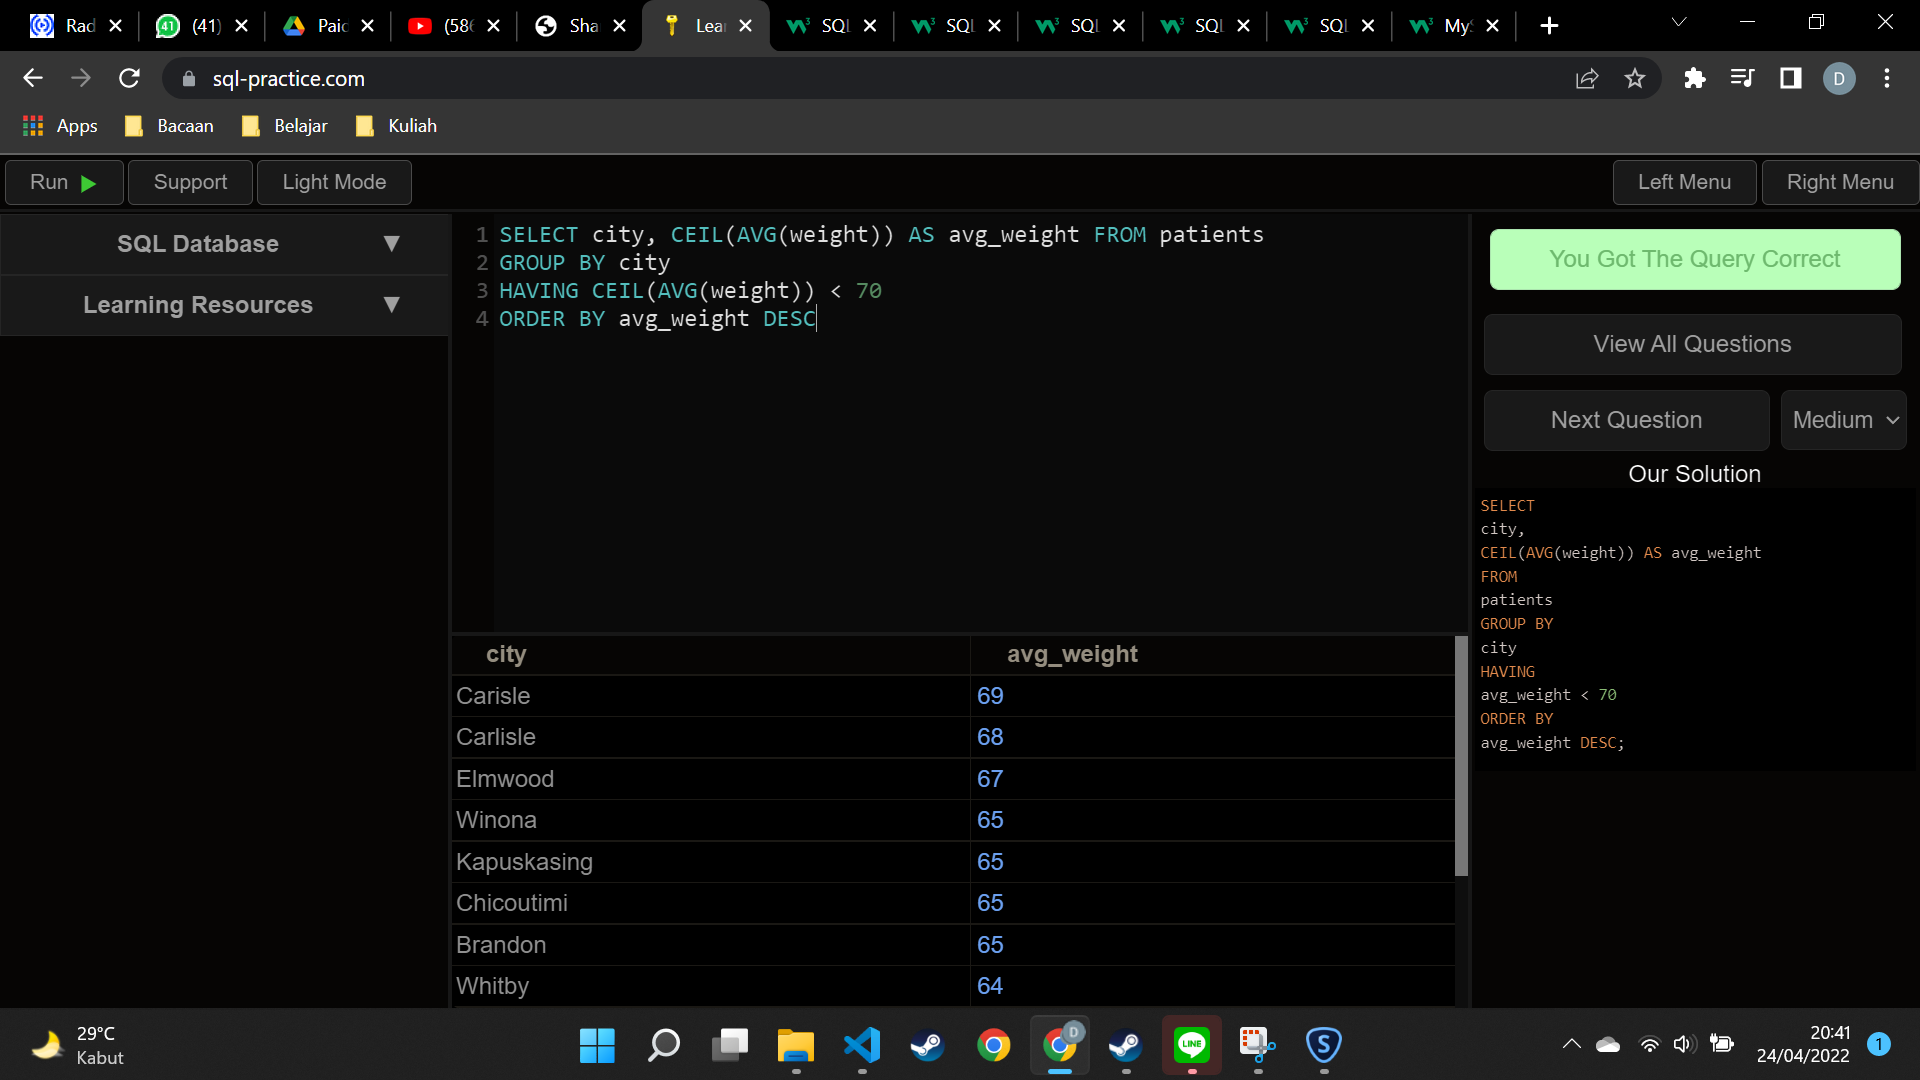
\includegraphics[scale=0.3]{./Screenshot/Medium-14.png}
            \centering
        \end{figure}

        \item Show the province\_id(s) where the total sum of its patient's height is greater than or equal to 7,000.
        \\Query :
        \lstinputlisting[label={listing26},caption={Medium - 15}, language={sql}]{"../Medium-15.sql"}
        \begin{itemize}
            \item Baris 1 : Mengambil data province\_id, jumlah dari height (akan disebut sebagai sum\_height) dari tabel patients
            \item Baris 2 : Mengelompokkan data berdasarkan province\_id
            \item Baris 3 : Dengan kondisi dimana sum\_height lebih dari 7000
        \end{itemize}
        \pagebreak
        Screenshot :
        \begin{figure}[h]
            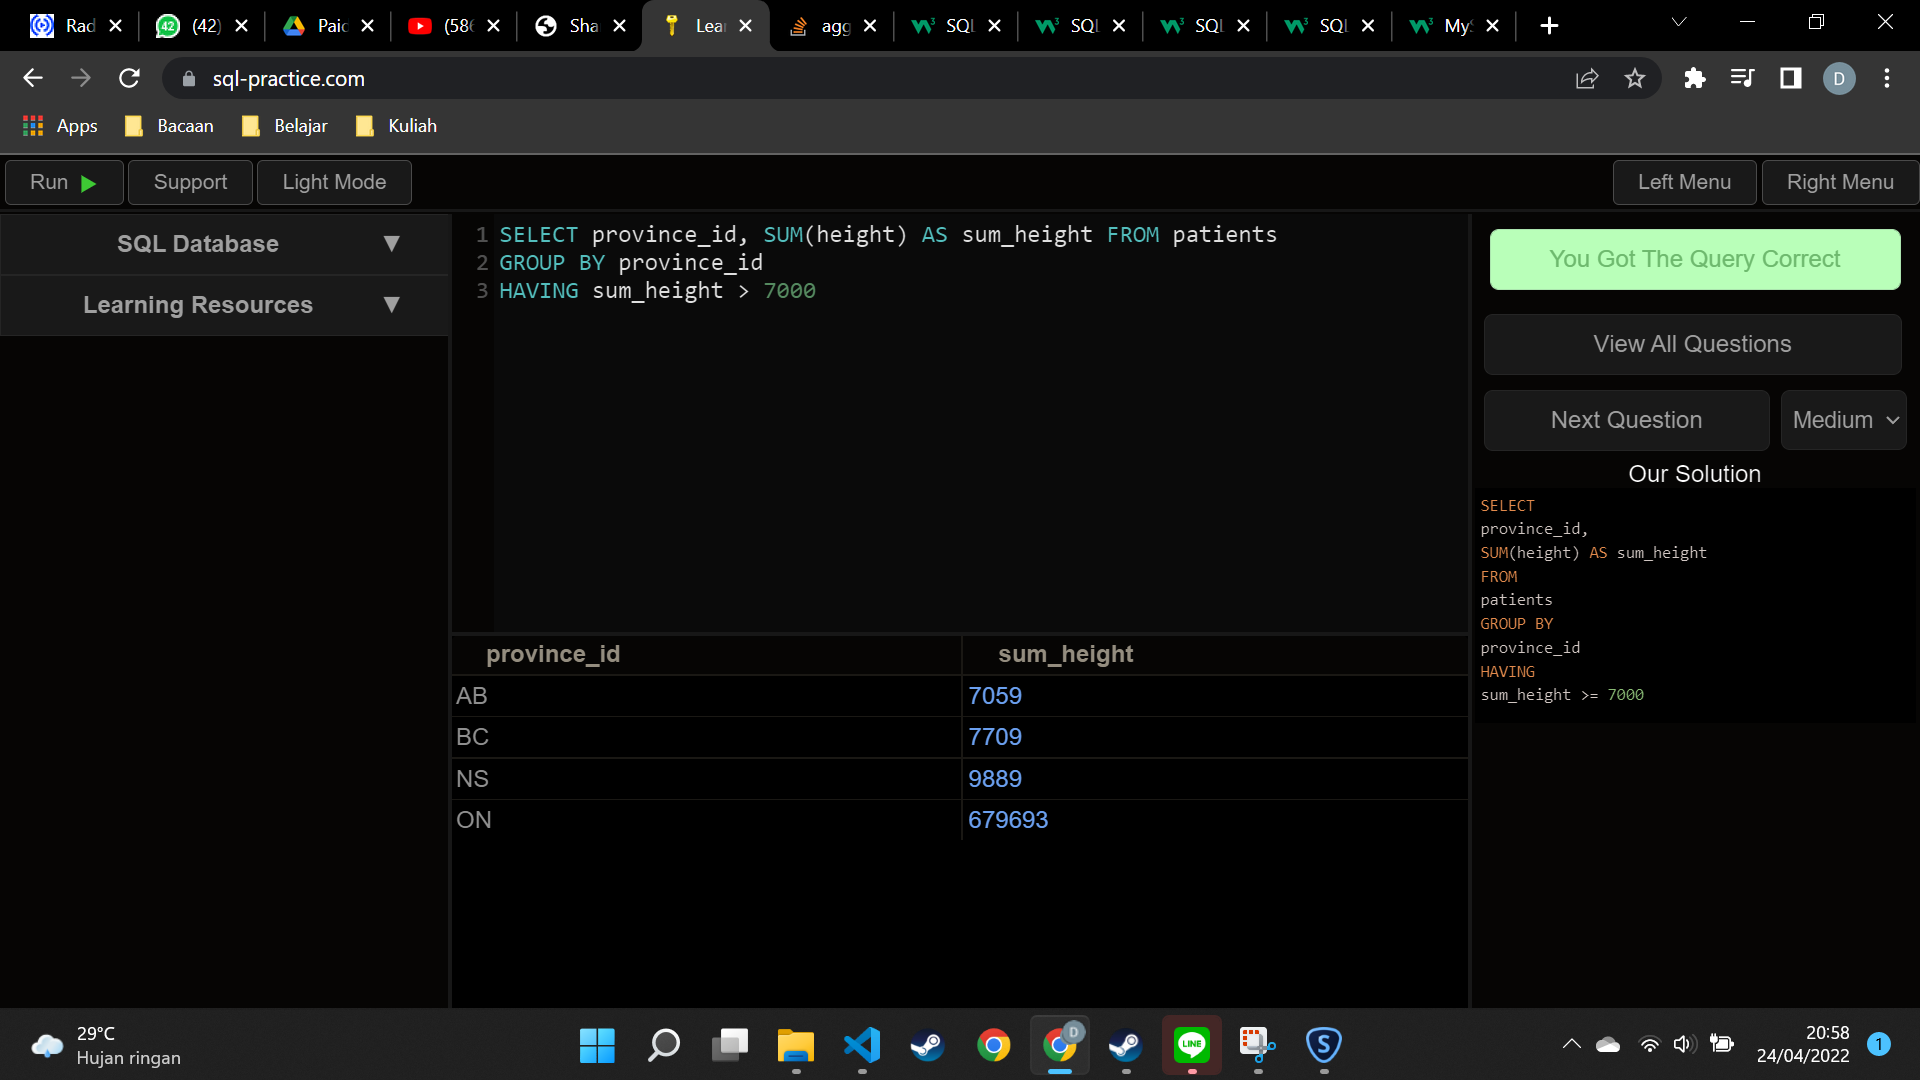
\includegraphics[scale=0.3]{./Screenshot/Medium-15.png}
            \centering
        \end{figure}

        \item Show the difference between the largest weight and smallest weight for patients with the last name 'Maroni'
        \\Query :
        \lstinputlisting[label={listing27},caption={Medium - 16}, language={sql}]{"../Medium-16.sql"}
        \begin{itemize}
            \item Baris 1 : Mengambil data selisih dari nilai maximal dengan nilai minimal dari kolom weight (akan disebut sebagai weight\_delta) dari tabel patients
            \item Baris 2 : Dengan kondisi dimana last\_name dari pasien adalah "Maroni"
        \end{itemize}
        \pagebreak
        Screenshot :
        \begin{figure}[h]
            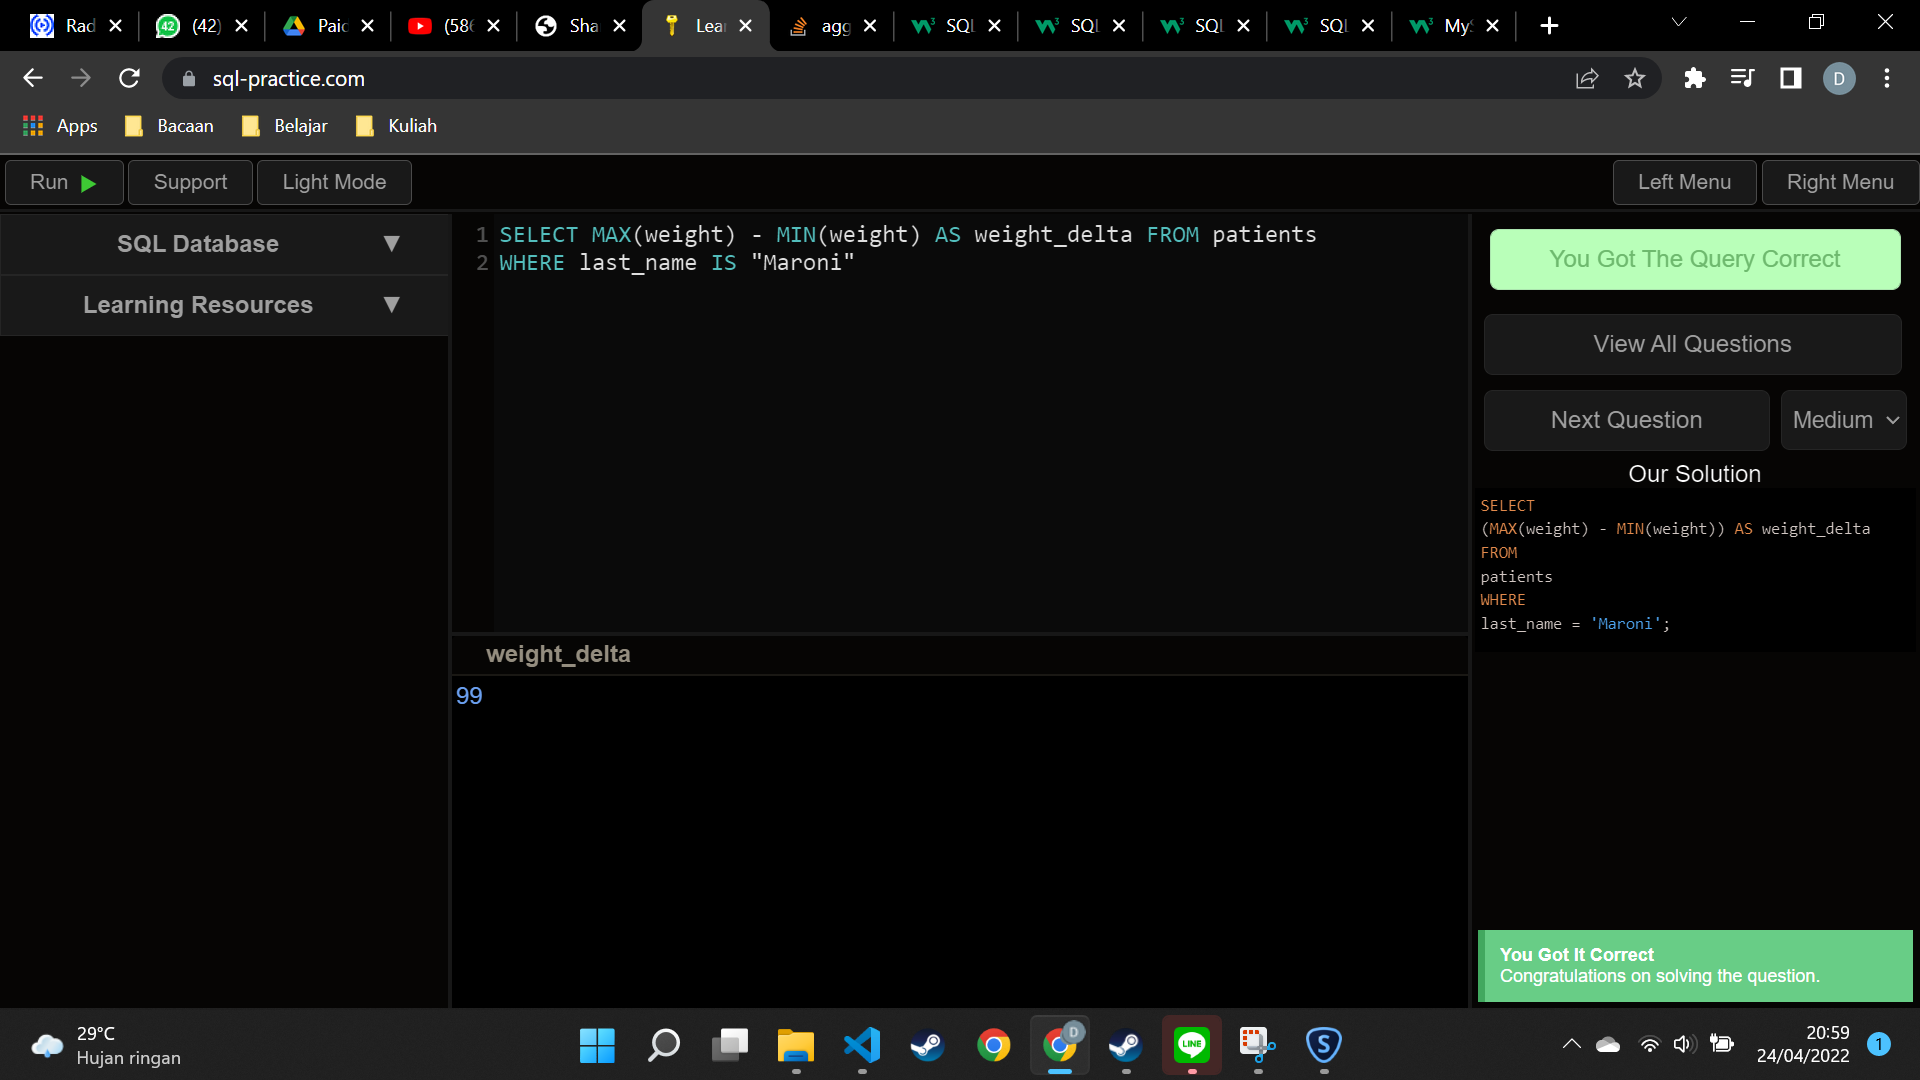
\includegraphics[scale=0.3]{./Screenshot/Medium-16.png}
            \centering
        \end{figure}

        \item Based on the cities that our patients live in, show unique cities that are in province\_id 'NS'?
        \\Query :
        \lstinputlisting[label={listing28},caption={Medium - 17}, language={sql}]{"../Medium-17.sql"}
        \begin{itemize}
            \item Baris 1 : Mengambil data yang unik pada kolom city dari tabel patients  
            \item Baris 2 : Dengan kondisi dimana province\_id dari pasien adalah "NS"
        \end{itemize}
        Screenshot :
        \begin{figure}[h]
            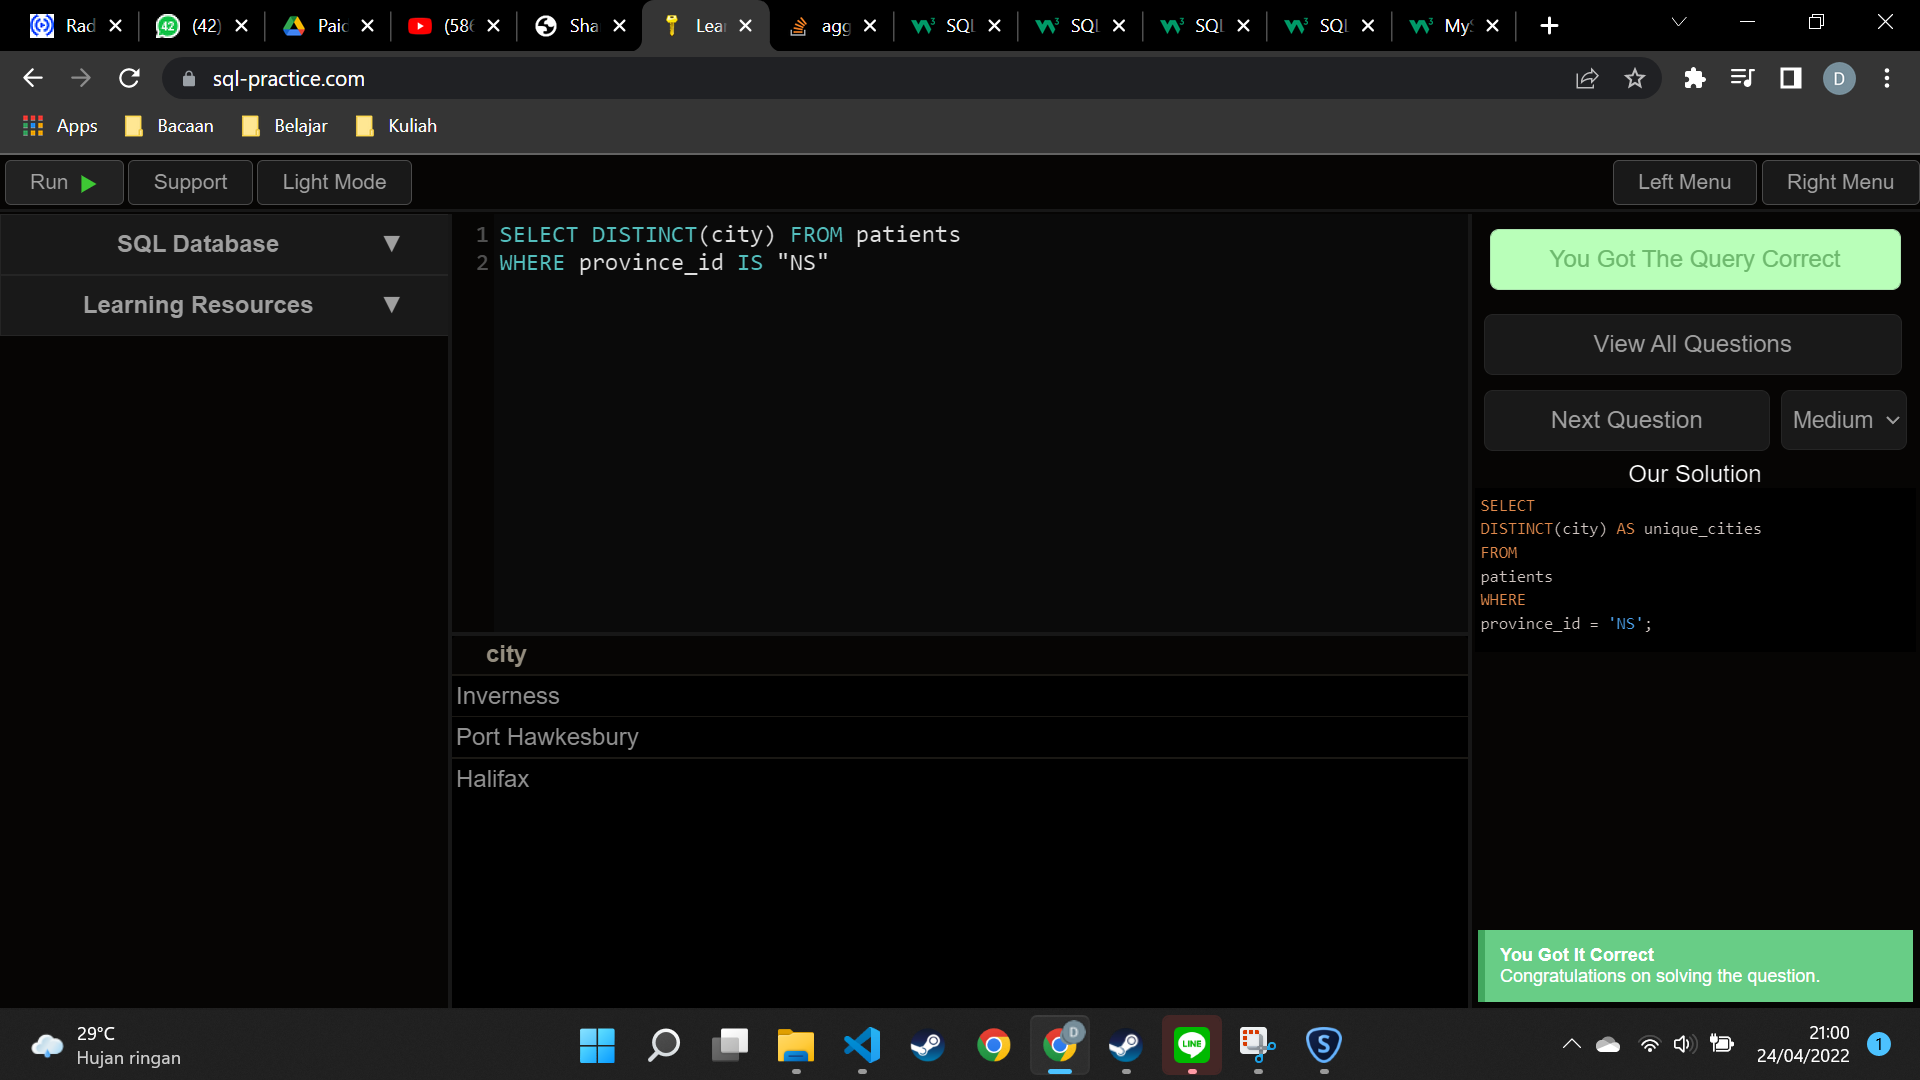
\includegraphics[scale=0.3]{./Screenshot/Medium-17.png}
            \centering
        \end{figure}

    \end{itemize}

\section{Soal Hard}
    \begin{itemize}
        \item Show all of the patients grouped into weight groups. Show the total amount of patients in each weight group. Order the list by the weight group decending. For example, if they weight 100 to 109 they are placed in the 100 weight group, 110-119 = 110 weight group, etc
        \\Query :
        \lstinputlisting[label={listing29},caption={Hard - 1}, language={sql}]{"../Hard-1.sql"}
        \begin{itemize}
            \item Baris 1 : Mengambil data table patients
            \item Baris 2 : Menambahkan kolom weight\_group sebagai tipe data integer pada table patients
            \item Baris 3 : Mengupdate table patients
            \item Baris 4 - 20 : Mengubah nilai weight\_group sesuai dengan berat pasien (menurut aturan dari soal)
            \item Baris 21 : Mengambil banyaknya data (akan disebut sebagai patients\_in\_group) dan weight\_group dari tabel patients
            \item Baris 22 : Mengelompokkan data berdasarkan weight\_group
            \item Baris 23 : Mengurutkan data berdasarkan weight\_group secara descending
        \end{itemize}
        \pagebreak
        Screenshot :
        \begin{figure}[h]
            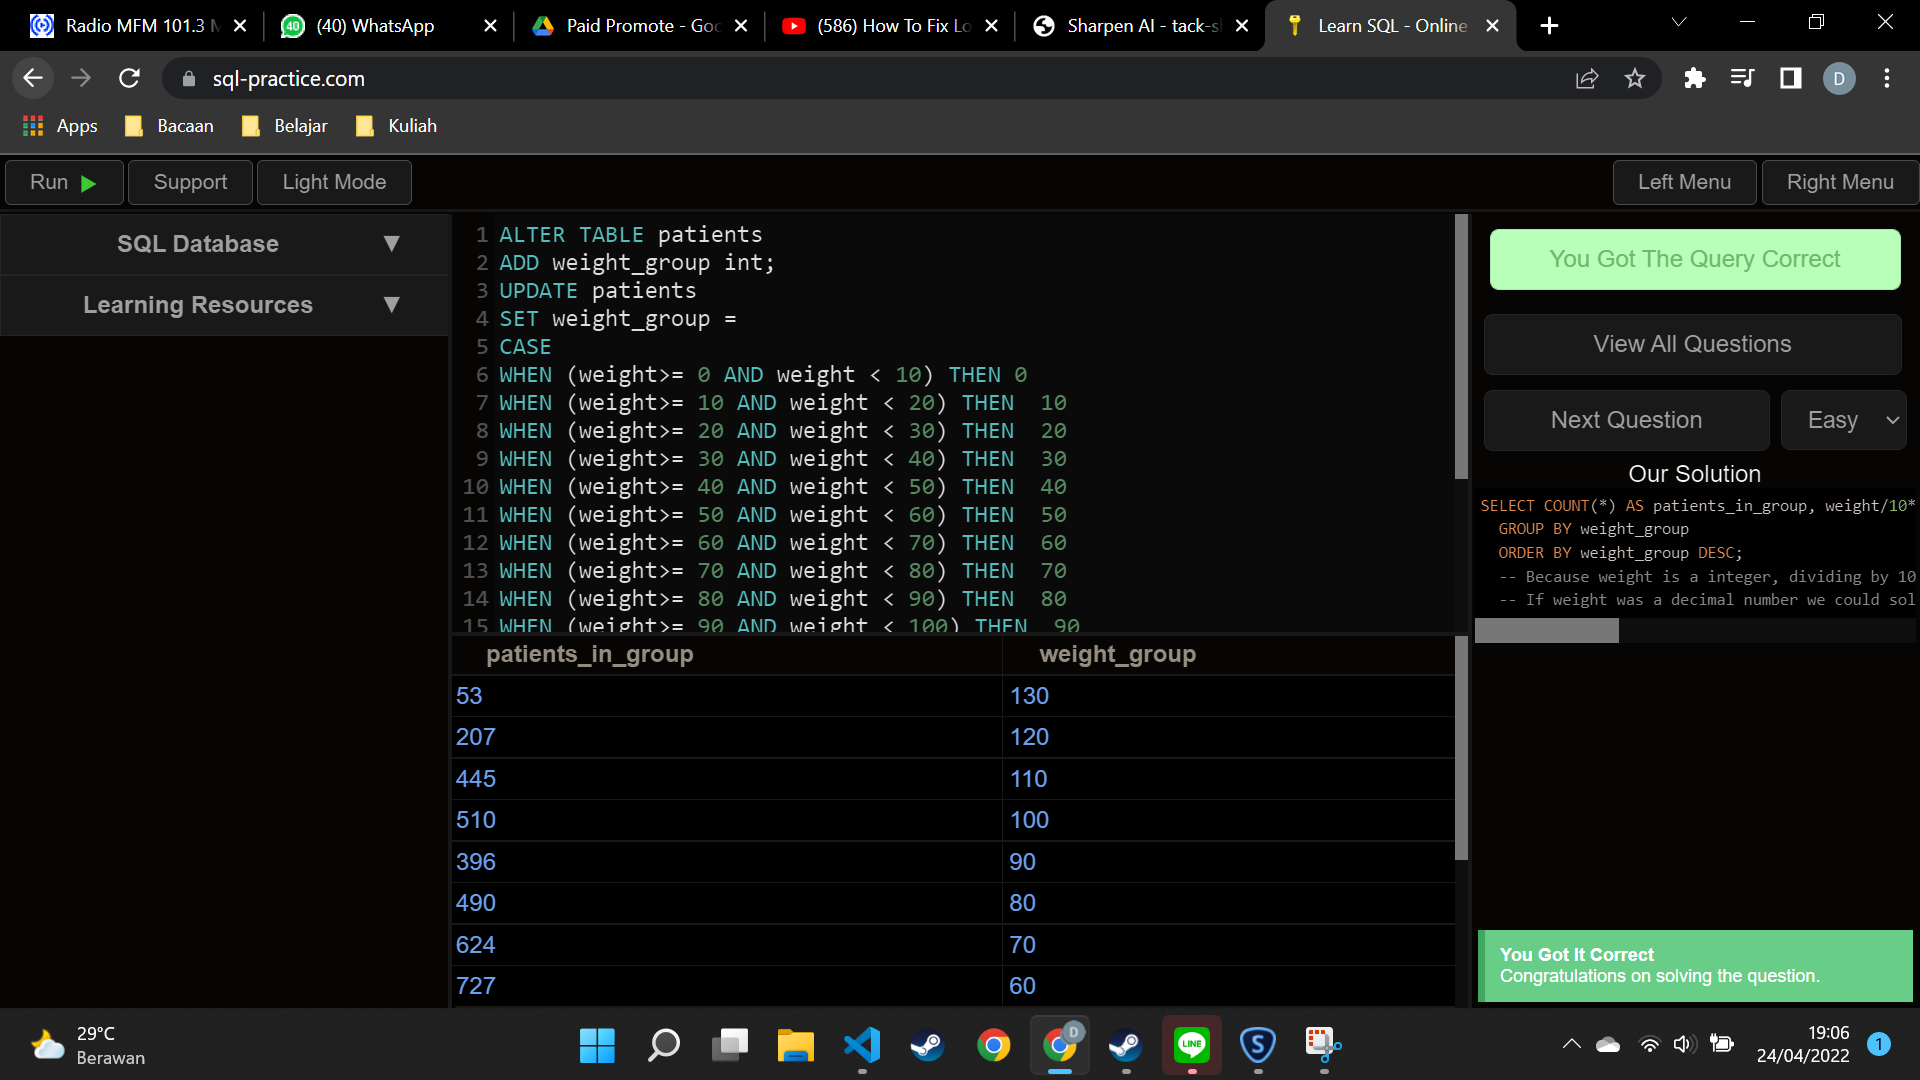
\includegraphics[scale=0.3]{./Screenshot/Hard-1.png}
            \centering
        \end{figure}

        \item Show patient\_id, weight, height, isObese from the patients table. Display isObese as a boolean 0 or 1. Obese is defined as weight(kg)/(height(m)$\textsuperscript{2}$) $>=$ 30. weight is in units kg. height is in units cm
        \\Query :
        \lstinputlisting[label={listing30},caption={Hard - 2}, language={sql}]{"../Hard-2.sql"}
        \begin{itemize}
            \item Baris 1 : Mengambil data patient\_id, weight, height, dan
            \\ $(weight/(height/100)\textsuperscript{2}) >= 30$ (akan disebut sebagai isObese) dari tabel patients
        \end{itemize}
        \pagebreak
        Screenshot :
        \begin{figure}[h]
            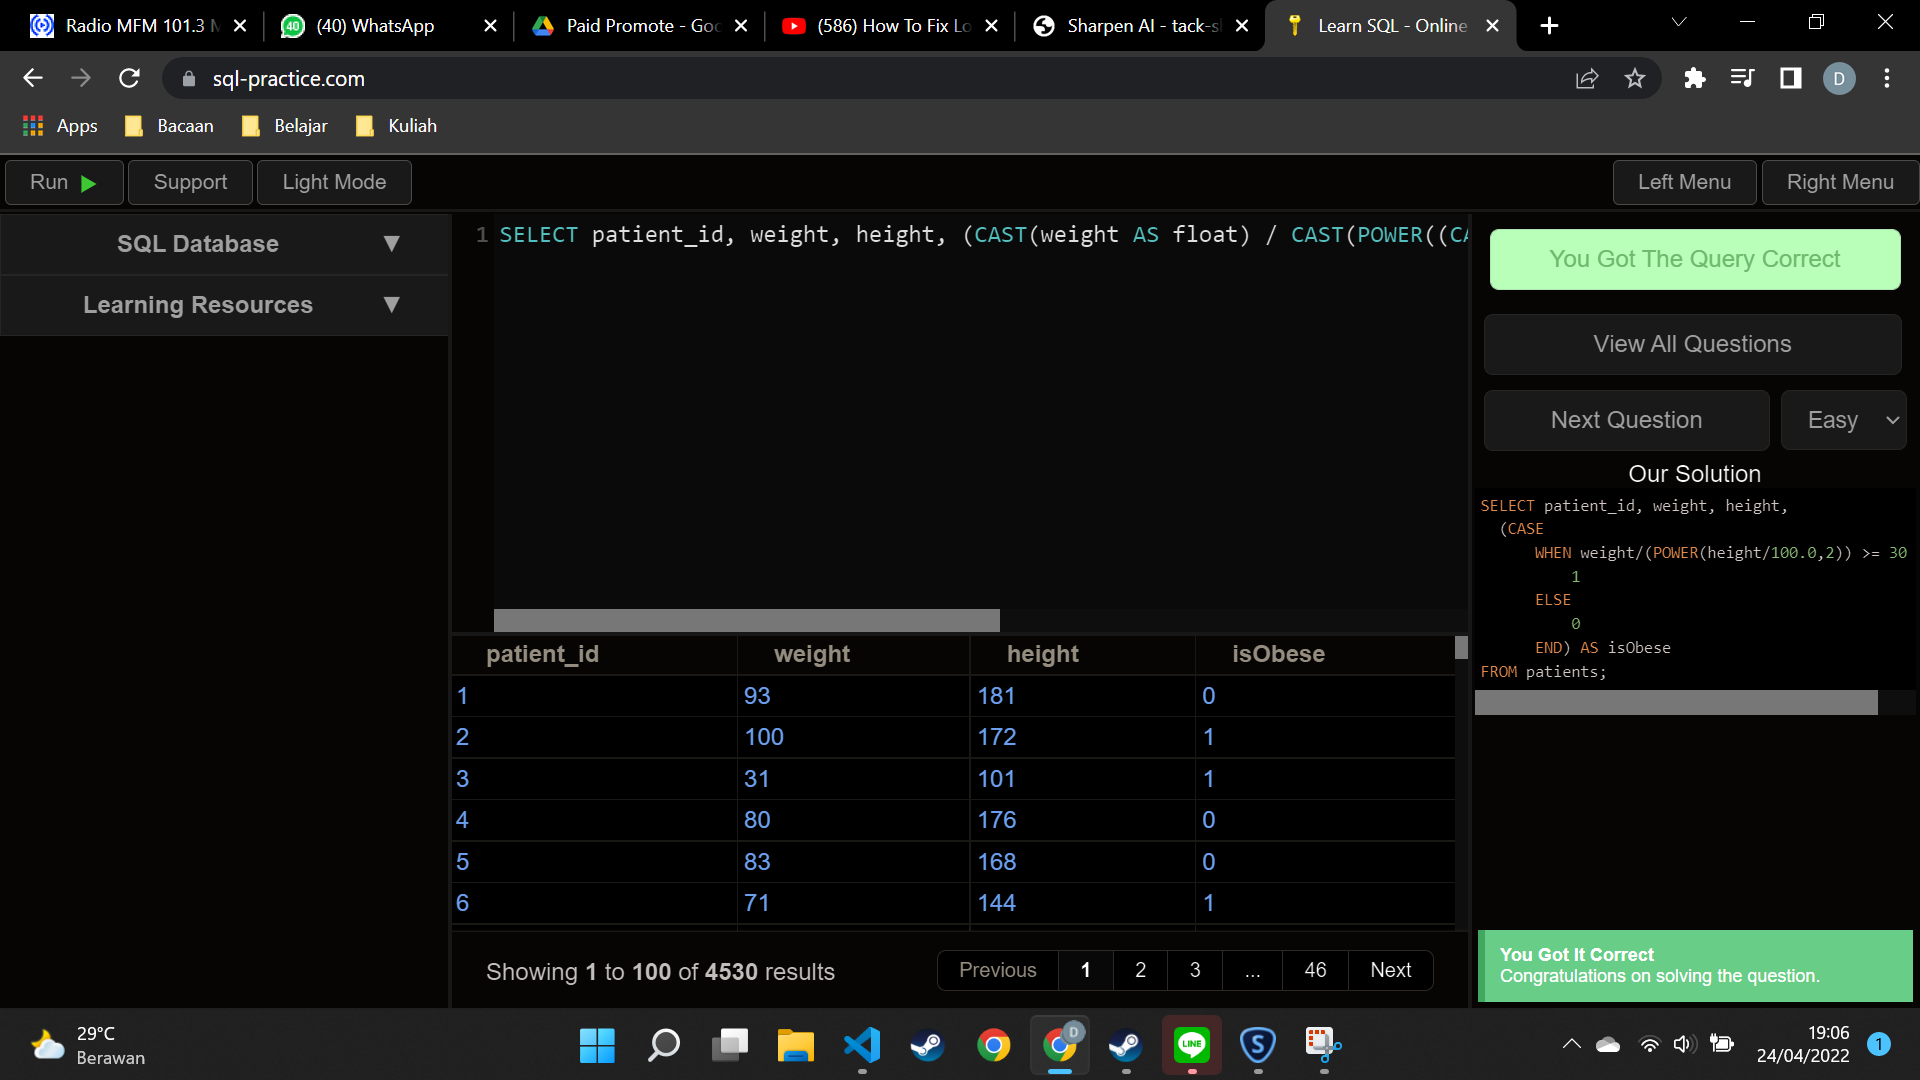
\includegraphics[scale=0.3]{./Screenshot/Hard-2.png}
            \centering
        \end{figure}

        \item Show patient\_id, first\_name, last\_name, and attending physician's specialty. Show only the patients who has a primary\_diagnosis as 'Dementia' and the physician's first name is 'Lisa'. Check patients, admissions, and physicians tables for required information.
        \\Query :
        \lstinputlisting[label={listing31},caption={Hard - 3}, language={sql}]{"../Hard-3.sql"}
        \begin{itemize}
            \item Baris 1 : Mengambil data patient\_id, first\_name, last\_name, dan specialty
            \item Baris 2 - 4 : Dari tabel admissions yang digabung dengan tabel patients dengan acuan patient\_id pada tabel admissions merujuk ke patient\_id pada tabel patients
            \item Baris 5 - 6 : Lalu digabung lagi dengan tabel physicians dengan acuan attending\_physician\_id pada tabel admissions merujuk ke physician\_id pada tabel physicians
            \item Baris 7 : Dengan kondisi dimana primary\_diagnosis dari pasien adalah "Dementia" dan first\_name dari physician adalah "Lisa"
        \end{itemize}
        \pagebreak
        Screenshot :
        \begin{figure}[h]
            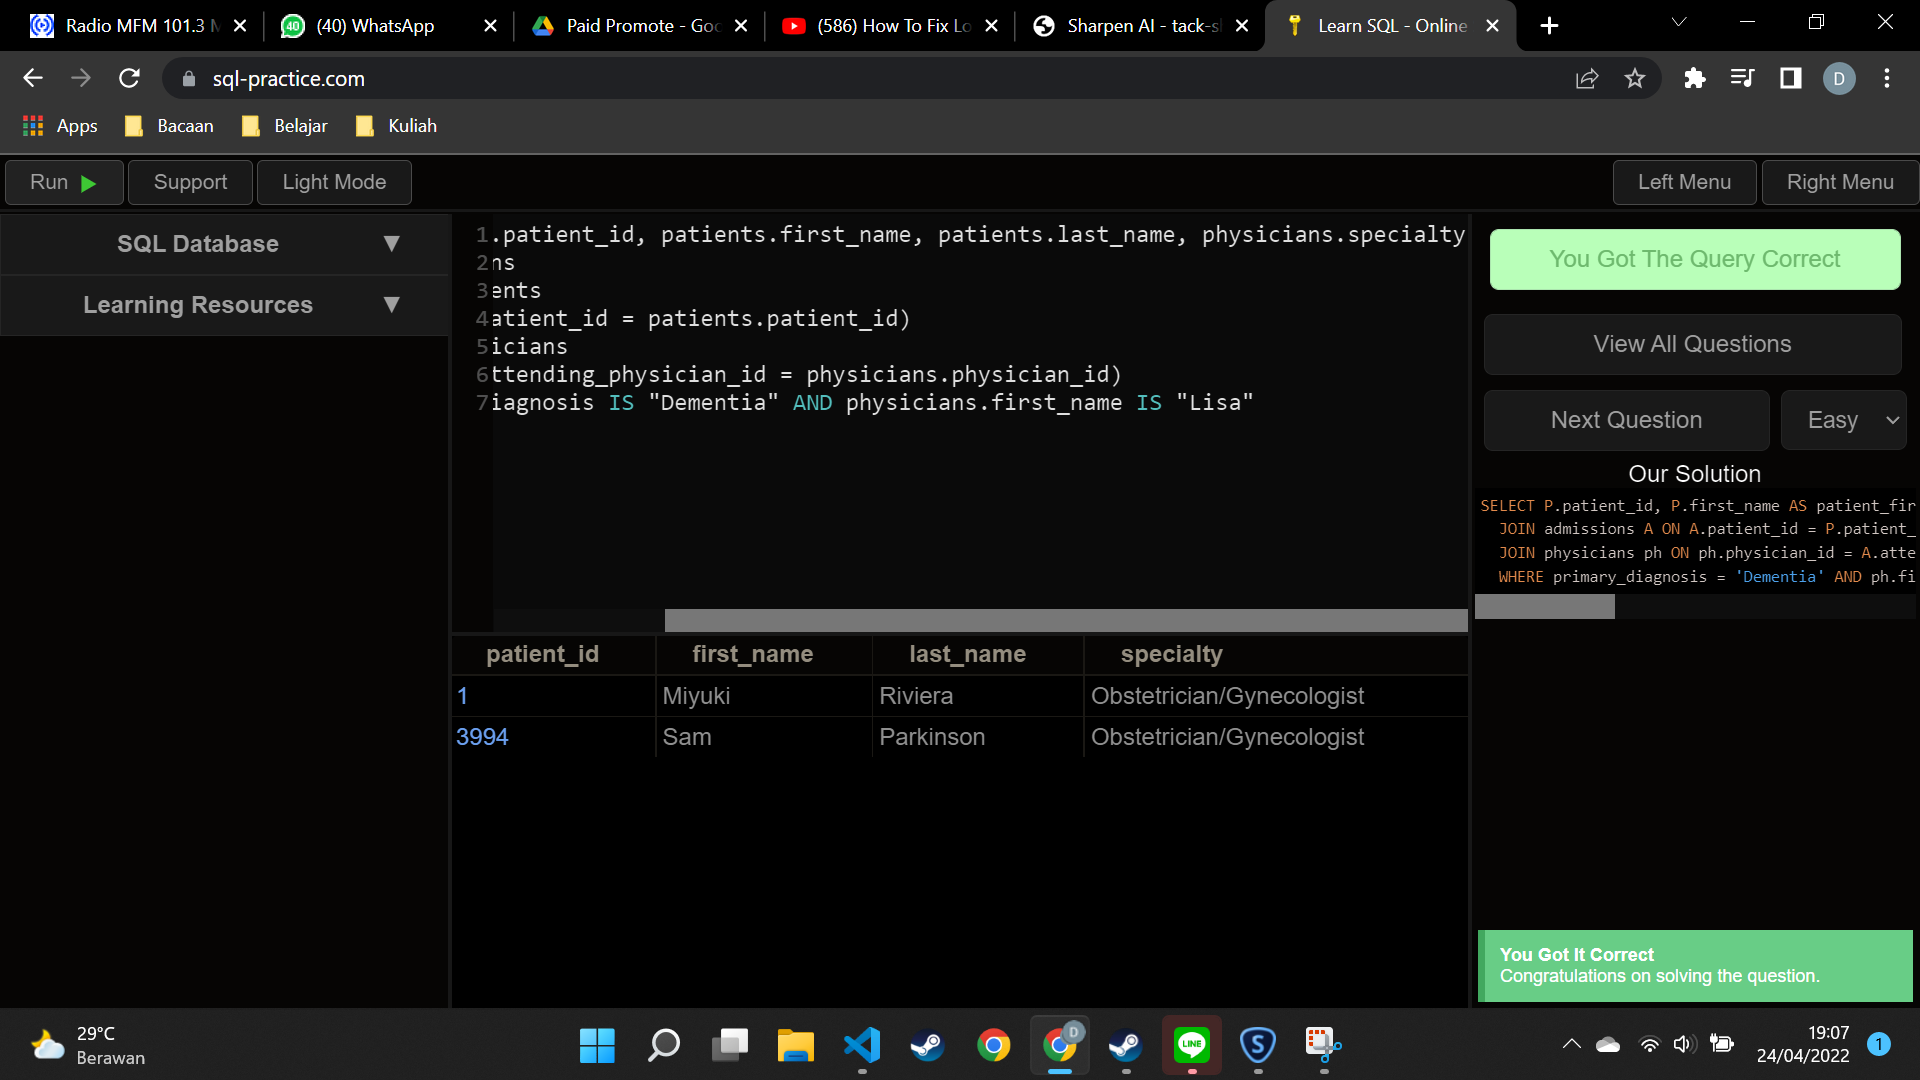
\includegraphics[scale=0.3]{./Screenshot/Hard-3.png}
            \centering
        \end{figure}

        \item All patients who have gone through admissions, can see their medical documents on our site. Those patients are given a temporary password after their first admission. Show the patient\_id and temp\_password.
        The password must be the following, in order:
            1. patient\_id
            2. the numerical length of patient's last\_name
            3. year of patient's birth\_date
        \\Query :
        \lstinputlisting[label={listing32},caption={Hard - 4}, language={sql}]{"../Hard-4.sql"}
        \begin{itemize}
            \item Baris 1 : Mengambil data unik dari kolom patient\_id, gabungan dari patient\_id, panjang last\_name dan tahun lahir (akan disebut sebagai temp\_password)
            \item Baris 2 : Dari tabel admissions
            \item Baris 3 : Menggabungkan tabel patients sesuai dengan data pada tabel admissions
            \item Baris 4 : Dengan acuan patient\_id pada tabel admissions merujuk ke patient\_id pada tabel patients
        \end{itemize}
        \pagebreak
        Screenshot :
        \begin{figure}[h]
            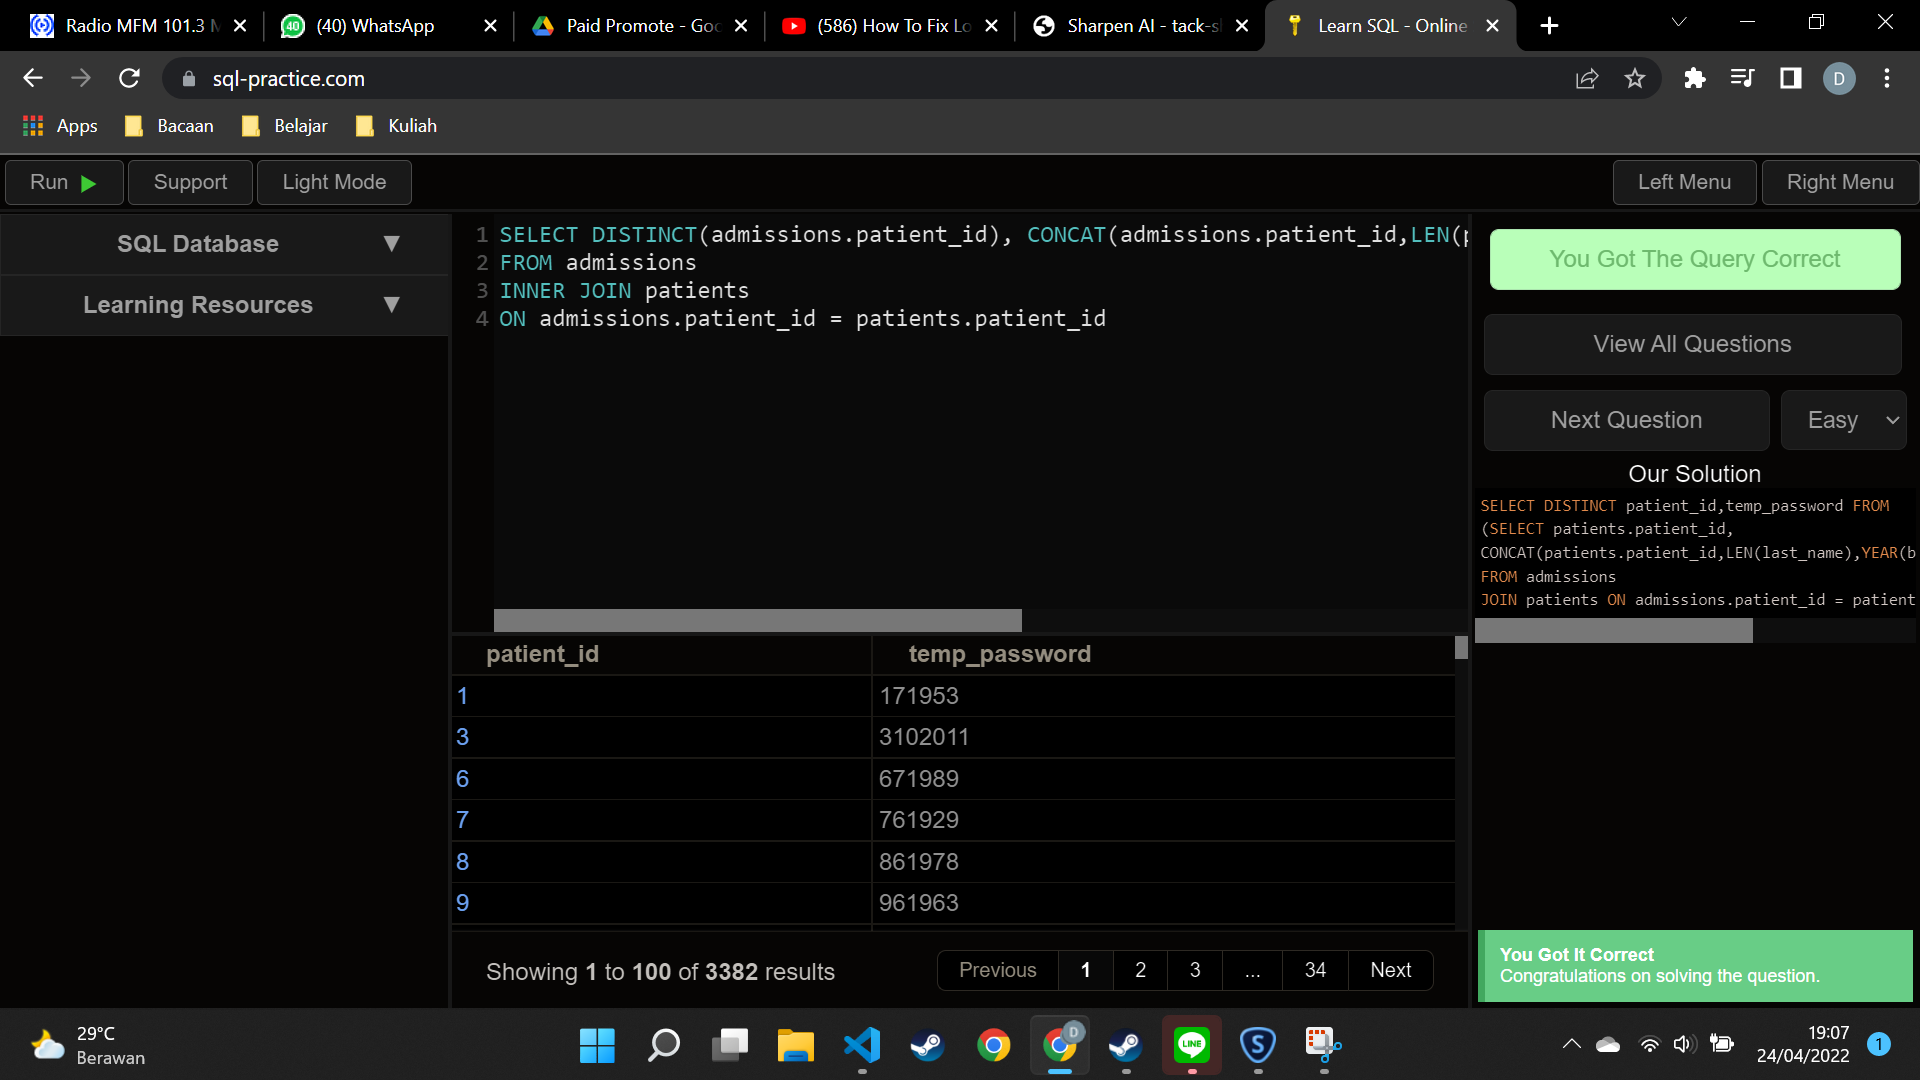
\includegraphics[scale=0.3]{./Screenshot/Hard-4.png}
            \centering
        \end{figure}

        \item Each admission costs 50 dollars for patients without insurance, and 10 dollars for patients with insurance. All patients with an even patient\_id have insurance.Give each patient a 'Yes' if they have insurance, and a 'No' if they don't have insurance. Add up the admission\_total cost for each has\_insurance group.
        \\Query :
        \lstinputlisting[label={listing33},caption={Hard - 5}, language={sql}]{"../Hard-5.sql"}
        \begin{itemize}
            \item Baris 1 : Mengambil data tabel admissions
            \item Baris 2 : Menambahkan kolom has\_insurance sebagai tipe data varchar
            \item Baris 3 : mengambil data tabel admissions
            \item Baris 4 : Menambahkan kolom cost\_after\_insurance sebagai tipe data integer
            \item Baris 5 : Mengupdate tabel admissions
            \item Baris 6 - 10 : Mengubah nilai dari has\_insurance sesuai dengan patient\_id, ketika patient\_id genap maka bernilai "Yes", ketika patient\_id ganjil maka bernilai "No"
            \item Baris 11 - 15 : Mengubah nilai dari cost\_after\_insurance sesuai dengan patient\_id, ketika patient\_id genap maka bernilai 10, ketika patient\_id ganjil maka bernilai 50
            \item Baris 16 : Mengambil data has\_insurance dan jumlah dari \\cost\_after\_insurance dari tabel admissions
            \item Baris 17 : Mengelompokkan data berdasarkan has\_insurance
        \end{itemize}
        Screenshot :
        \begin{figure}[h]
            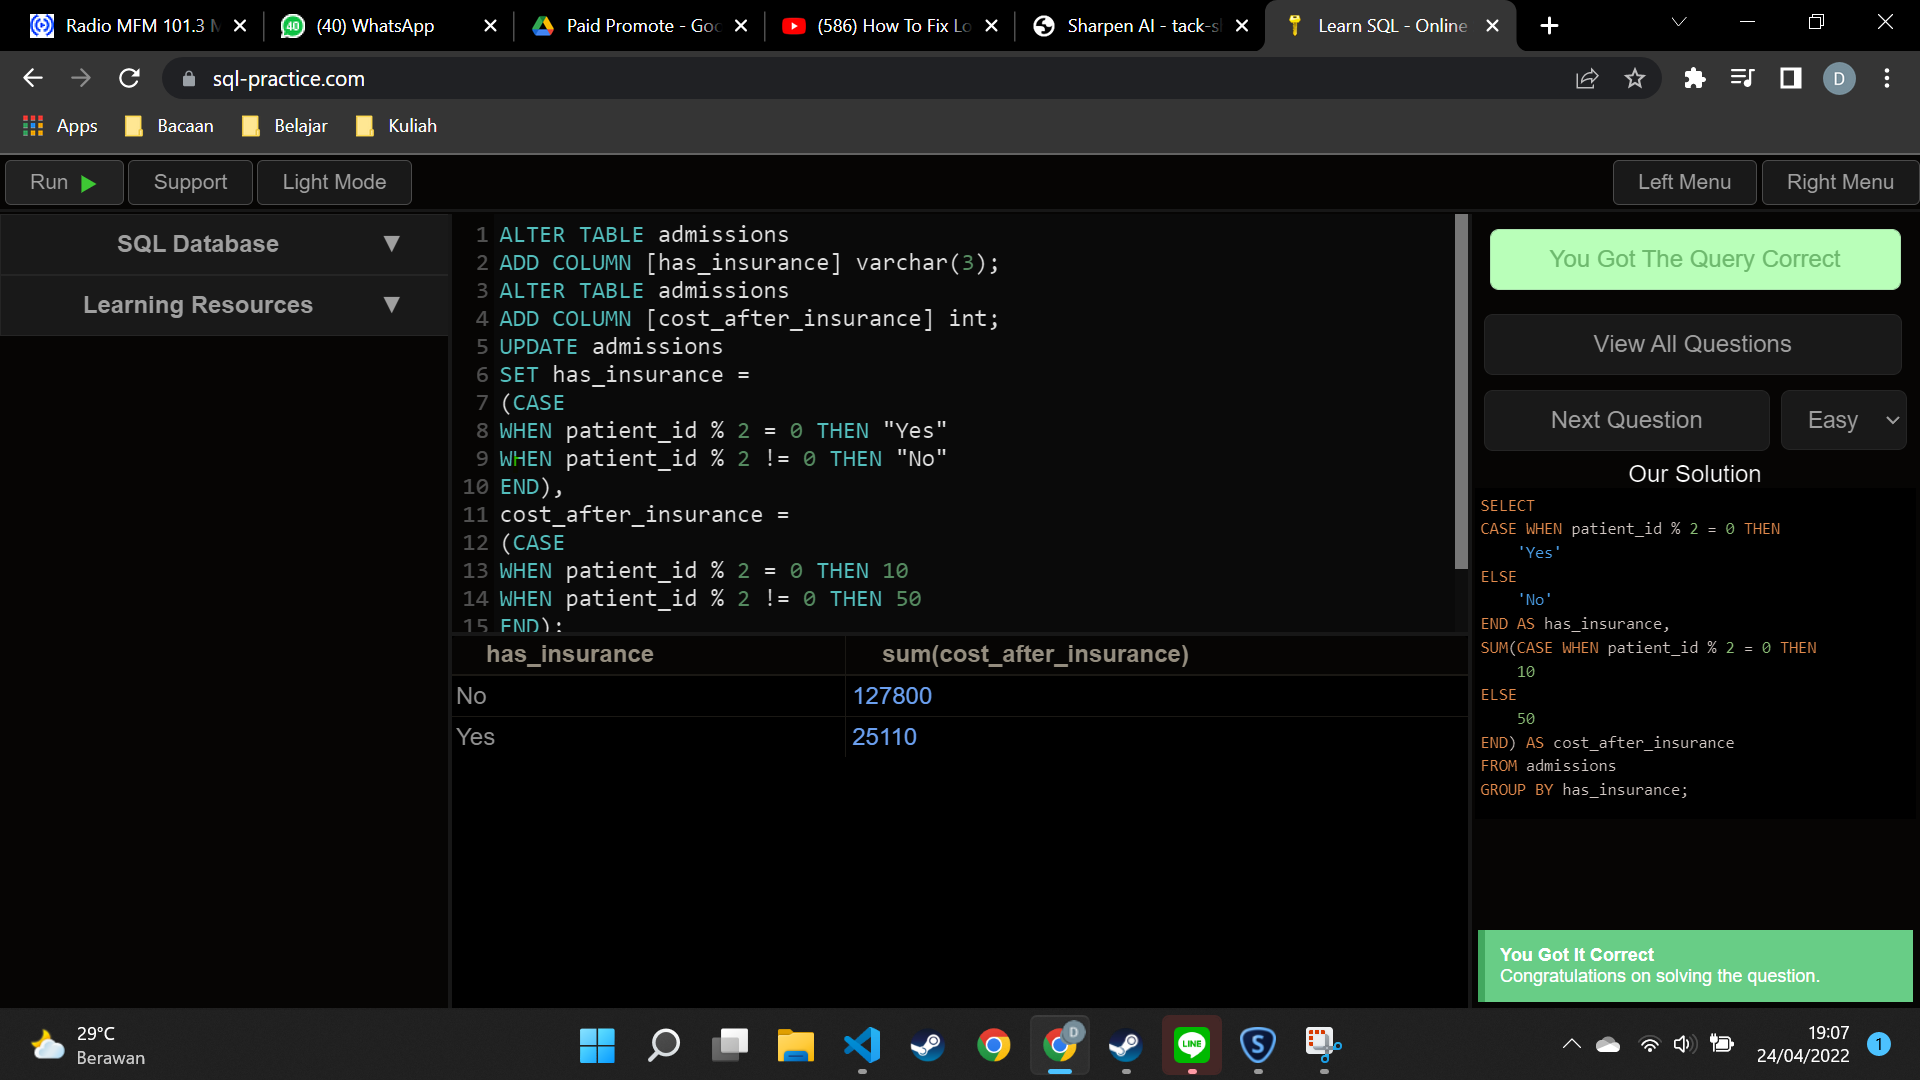
\includegraphics[scale=0.3]{./Screenshot/Hard-5.png}
            \centering
        \end{figure}

        \item Show the province that has more patients identified as 'M' than 'F'. Must only show full province\_name
        \\Query :
        \lstinputlisting[label={listing34},caption={Hard - 6}, language={sql}]{"../Hard-6.sql"}
        \begin{itemize}
            \item Baris 1 : Mengambil data province\_name dari tabel patients
            \item Baris 2 : Menggabungkan data pada tabel provinces sesuai dengan data pada tabel patients
            \item Baris 3 : Dengan acuan province\_id pada tabel patients merujuk ke province\_id pada tabel provinces
            \item Baris 4 : Mengelompokkan data berdasarkan province\_id
            \item Baris 5 : Dengan kondisi dimana banyaknya data dengan gender "M" lebih banyak dibandingkan data dengan gender "F"
        \end{itemize}
        Screenshot :
        \begin{figure}[h]
            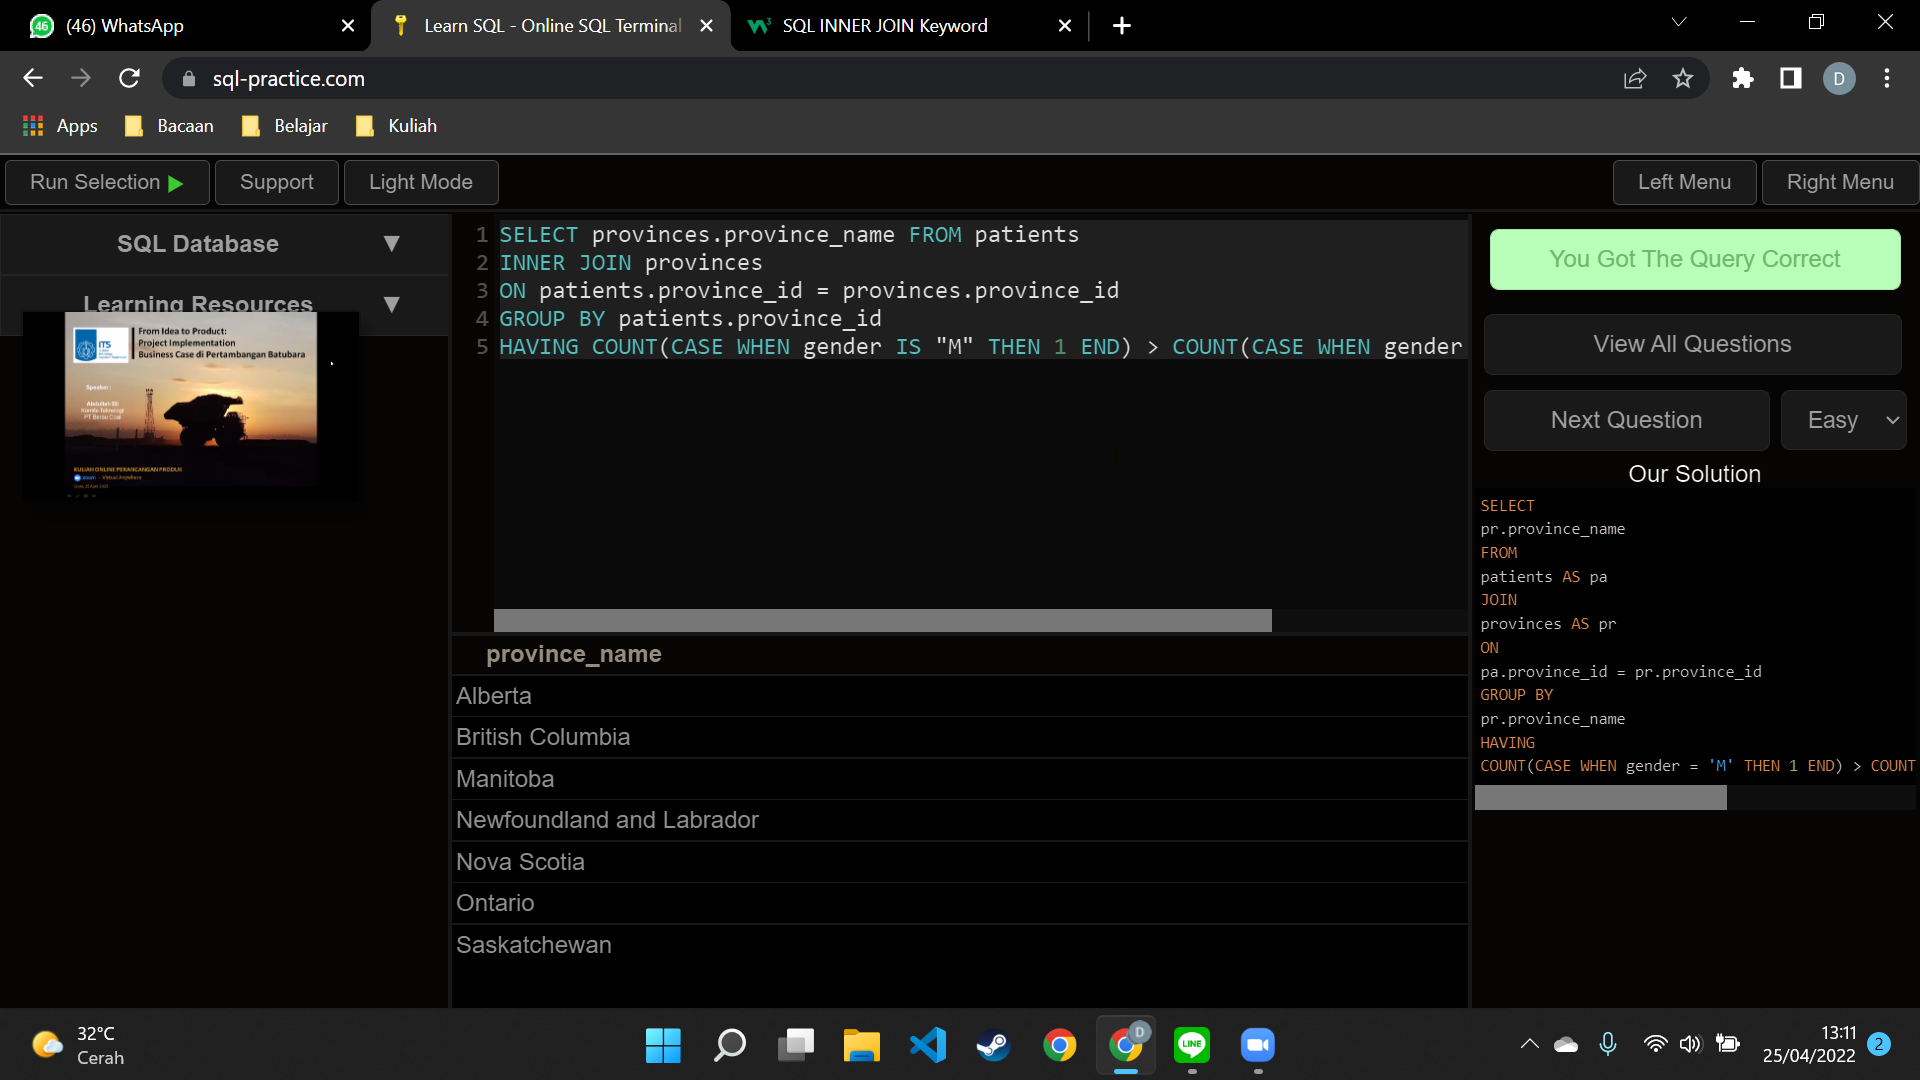
\includegraphics[scale=0.3]{./Screenshot/Hard-6.png}
            \centering
        \end{figure}

        \item We are looking for a specific patient. Pull all columns for the patient who matches the following criteria:
        \begin{itemize}
            \item First\_name contains an 'r' after the first two letters.
            \item Identifies their gender as 'F'
            \item Born in February, May, or December
            \item Their weight would be between 60kg and 80kg
            \item Their patient\_id is an odd number
            \item They are from the city 'Halifax'
        \end{itemize}
        Query :
        \lstinputlisting[label={listing35},caption={Hard - 7}, language={sql}]{"../Hard-7.sql"}
        \begin{itemize}
            \item Baris 1 : Mengambil semua data dari tabel patients
            \item Baris 2 : Dengan kondisi dimana first\_name yang mengandung huruf "r" pada huruf ketiga
            \item Baris 3 : Dan bergender "F"
            \item Baris 4 : Dan memiliki bulan lahir yang termasuk dalam (2, 3, 12)
            \item Baris 5 : Dan memiliki weight diantara 60 dan 80
            \item Baris 6 : Dan memiliki patient\_id ganjil
            \item Baris 7 : Dan berasal dari kota "Halifax"
        \end{itemize}
        Screenshot :
        \begin{figure}[h]
            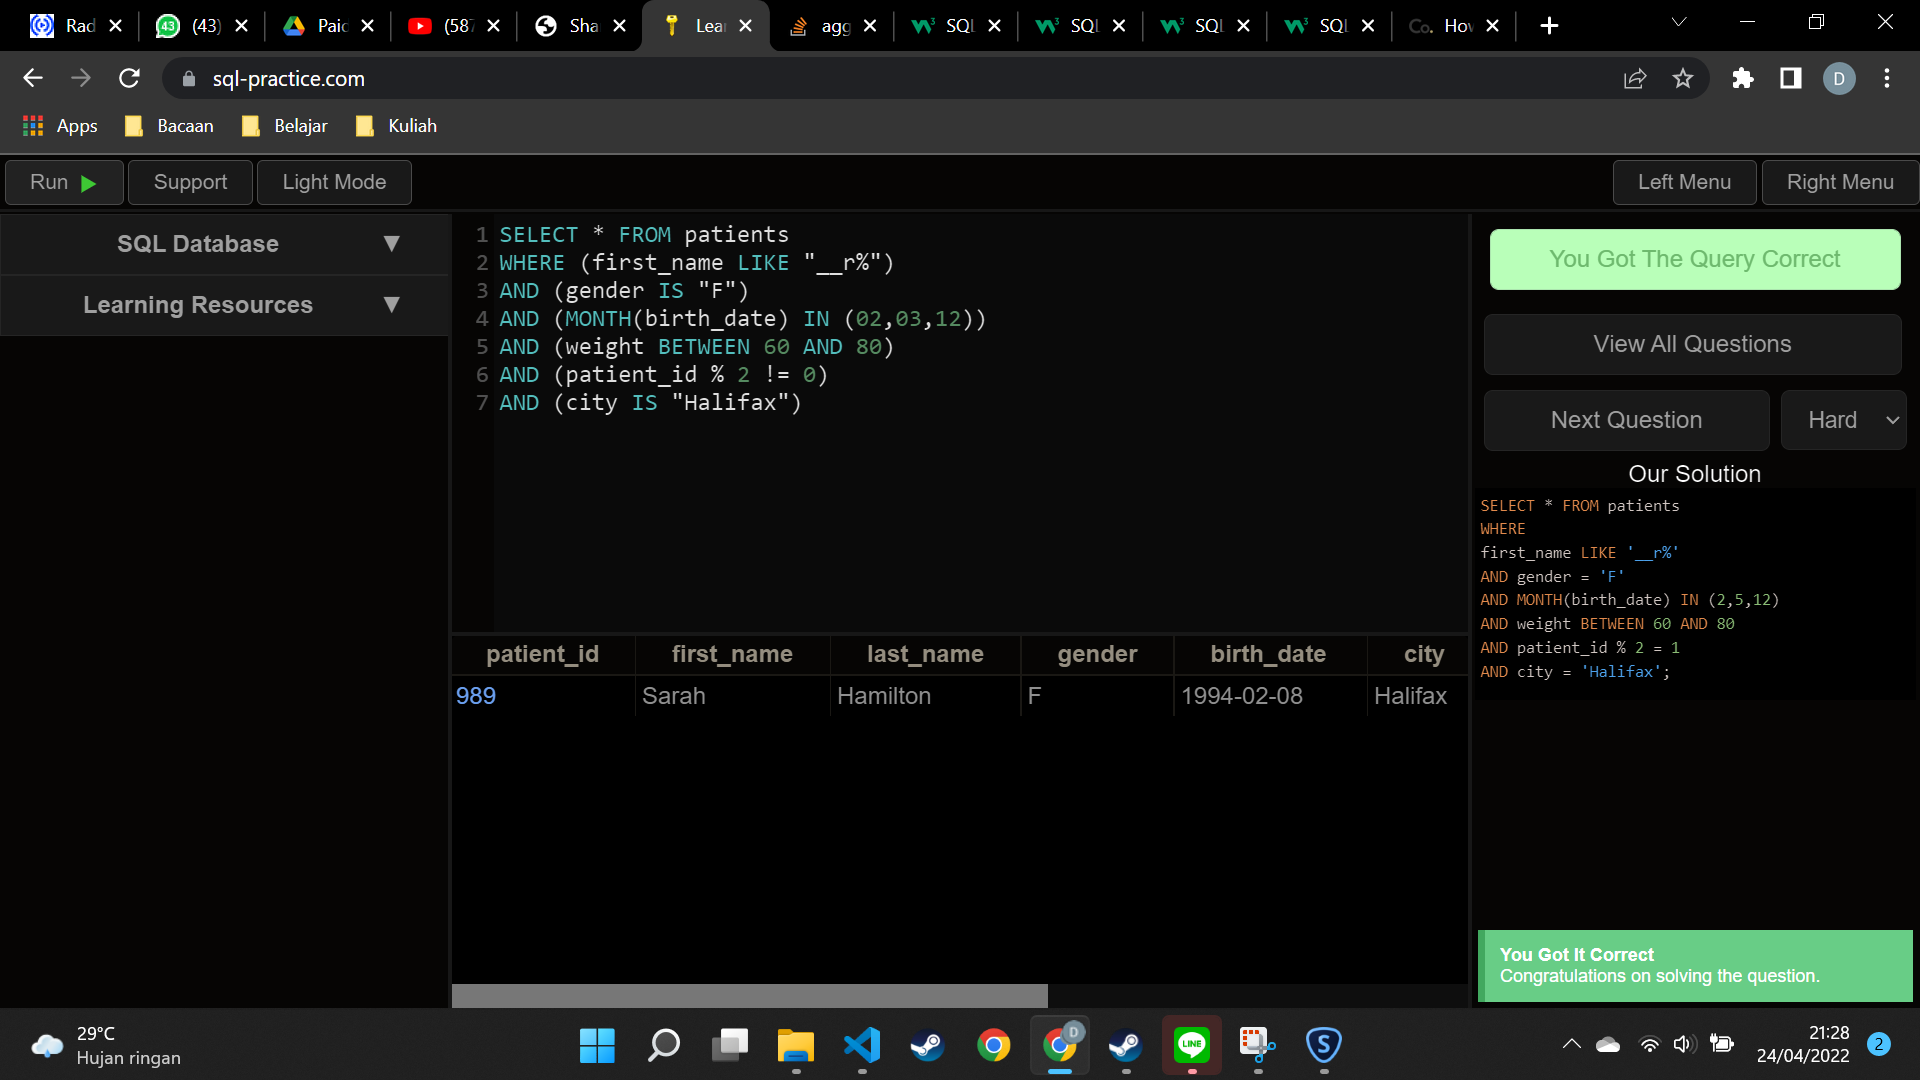
\includegraphics[scale=0.3]{./Screenshot/Hard-7.png}
            \centering
        \end{figure}

        \item Show the percent of patients that have 'M' as their gender. Round the answer to the nearest hundreth number and in percent form.
        \\Query :
        \lstinputlisting[label={listing36},caption={Hard - 8}, language={sql}]{"../Hard-8.sql"}
        \begin{itemize}
            \item Baris 1 : Mengambil data gabungan dari pembulatan pada 2 angka dibelakang koma dari perhitungan banyaknya data bergender "M" dibagi total banyaknya data dikali 100 (perhitungan persentase), dan tanda "\%" (akan disebut sebagai percent\_of\_male\_patients) dari tabel patients
        \end{itemize}
        \pagebreak
        Screenshot :
        \begin{figure}[h]
            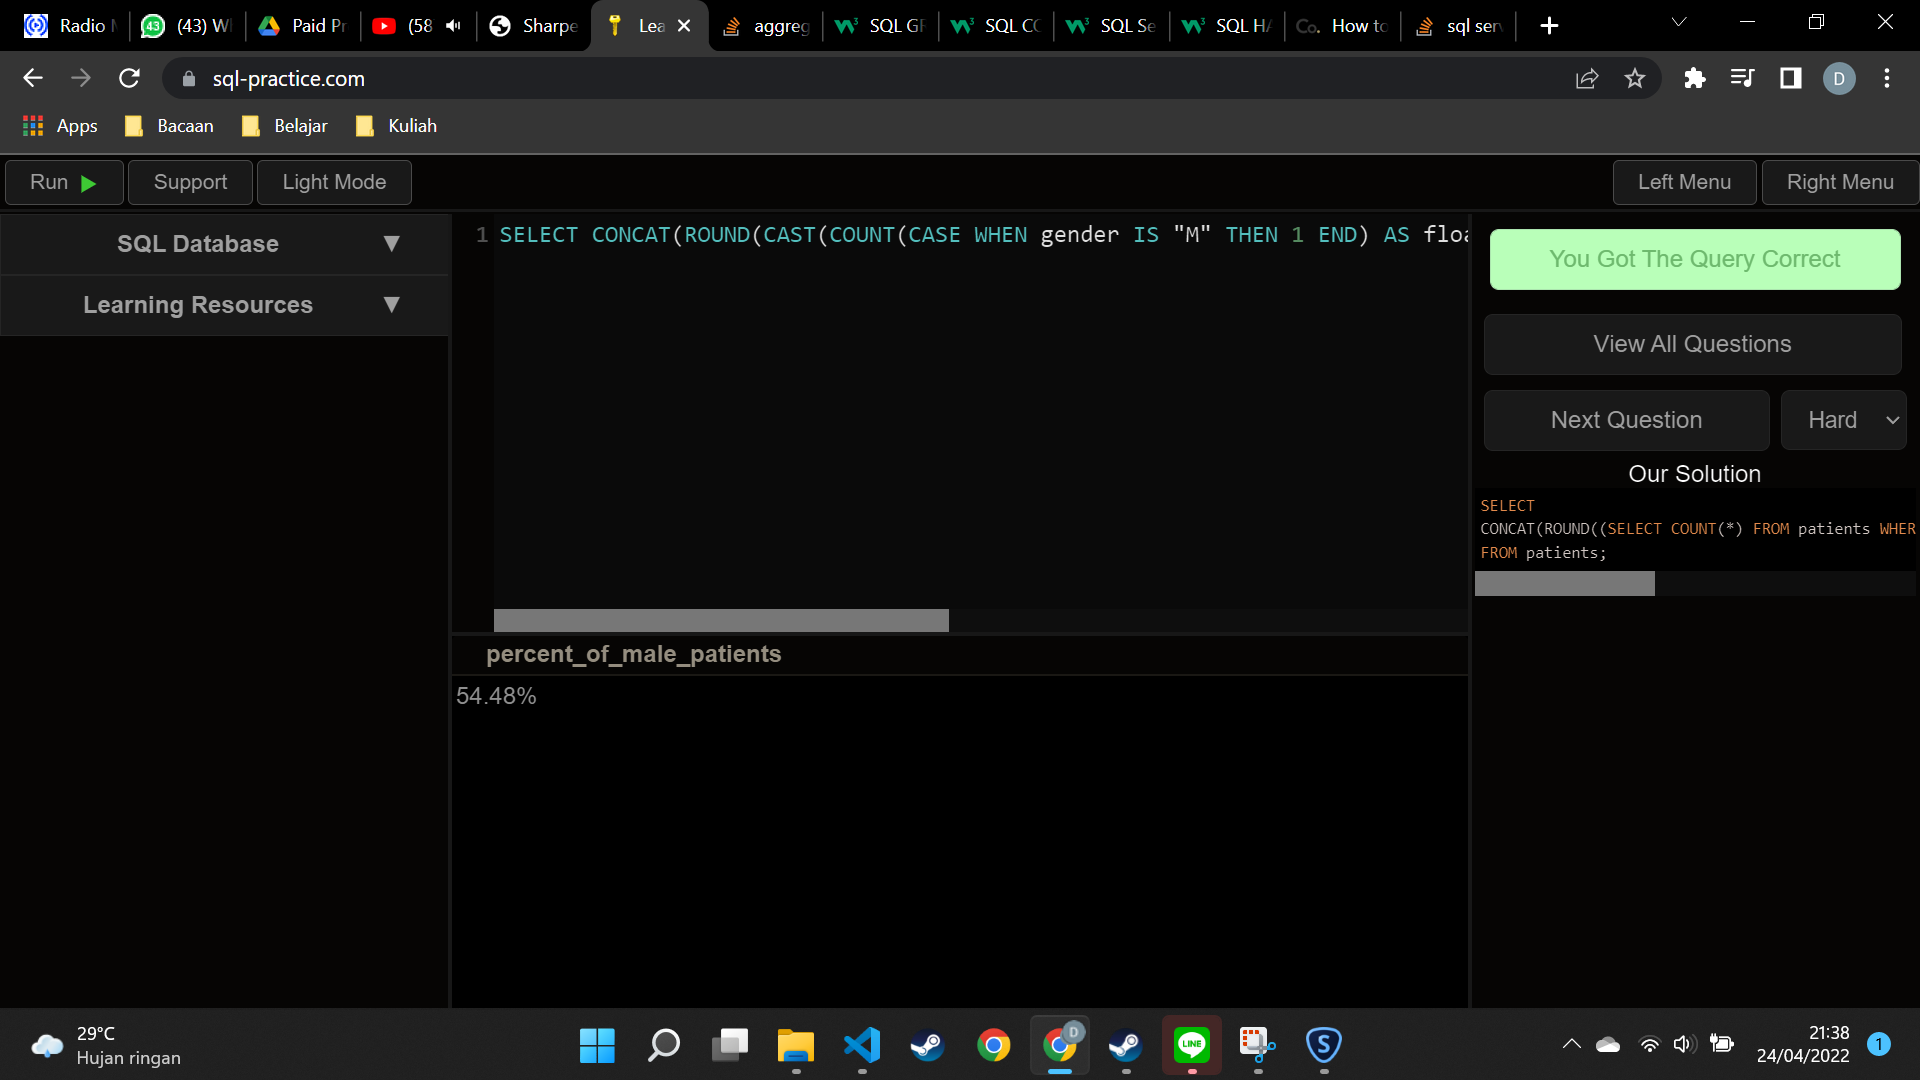
\includegraphics[scale=0.3]{./Screenshot/Hard-8.png}
            \centering
        \end{figure}

    \end{itemize}

\end{document}
